\documentclass[compress]{beamer}
\usepackage{ifthen,verbatim}

\newcommand{\isnote}{}
\xdefinecolor{lightyellow}{rgb}{1.,1.,0.25}
\xdefinecolor{darkblue}{rgb}{0.1,0.1,0.7}

%% Uncomment this to get annotations
%% \def\notes{\addtocounter{page}{-1}
%%            \renewcommand{\isnote}{*}
%% 	   \beamertemplateshadingbackground{lightyellow}{white}
%%            \begin{frame}
%%            \frametitle{Notes for the previous page (page \insertpagenumber)}
%%            \itemize}
%% \def\endnotes{\enditemize
%% 	      \end{frame}
%%               \beamertemplateshadingbackground{white}{white}
%%               \renewcommand{\isnote}{}}

%% Uncomment this to not get annotations
\def\notes{\comment}
\def\endnotes{\endcomment}

\setbeamertemplate{navigation symbols}{}
\setbeamertemplate{headline}{\mbox{ } \hfill
\begin{minipage}{5.5 cm}
\vspace{-0.75 cm} \small
\end{minipage} \hfill
\begin{minipage}{4.5 cm}
\vspace{-0.75 cm} \small
\begin{flushright}
\ifthenelse{\equal{\insertpagenumber}{1}}{}{Jim Pivarski \hspace{0.2 cm} \insertpagenumber\isnote/\pageref{numpages}}
\end{flushright}
\end{minipage}\mbox{\hspace{0.2 cm}}\includegraphics[height=1 cm]{../cmslogo} \hspace{0.1 cm} \includegraphics[height=1 cm]{../tamulogo} \hspace{0.01 cm} \vspace{-1.05 cm}}

\newcommand{\s}[1]{{\mbox{\scriptsize #1}}}

\begin{document}
\begin{frame}
\vfill
\begin{center}
\textcolor{darkblue}{\Large Muon Groups Analysis Update}

\vfill
\begin{columns}
\column{0.3\linewidth}
\begin{center}
\large
Jim Pivarski
\end{center}
\end{columns}

\begin{columns}
\column{0.3\linewidth}
\begin{center}
\scriptsize
{\it Texas A\&M University}
\end{center}
\end{columns}

\vfill
26 July, 2010

\end{center}
\end{frame}

%% \begin{notes}
%% \item This is the annotated version of my talk.
%% \item If you want the version that I am presenting, download the one
%% labeled ``slides'' on Indico (or just ignore these yellow pages).
%% \item The annotated version is provided for extra detail and a written
%% record of comments that I intend to make orally.
%% \item Yellow notes refer to the content on the {\it previous} page.
%% \item All other slides are identical for the two versions.
%% \end{notes}

\small

\begin{frame}
\frametitle{Outline}
\begin{itemize}
\item Corrections from last time
\item New studies of backgrounds
\end{itemize}
\end{frame}

\begin{frame}
\frametitle{Efficiency plots}
\framesubtitle{Corrections from last time}

\begin{description}
\item[Symptom:] StandAloneMuon efficiency seemed to fall off at high
  $\eta$, GlobalMuon efficiency was higher than StandAlone
\item[Problem:] numerator of ``efficiency'' required MC-matching
\item[Solution:] $\displaystyle \epsilon = \frac{\mbox{reconstructed 2 muons}}{\mbox{all generated}}$ (show vs.\ $pT_2$ and $\eta_1$)
\end{description}

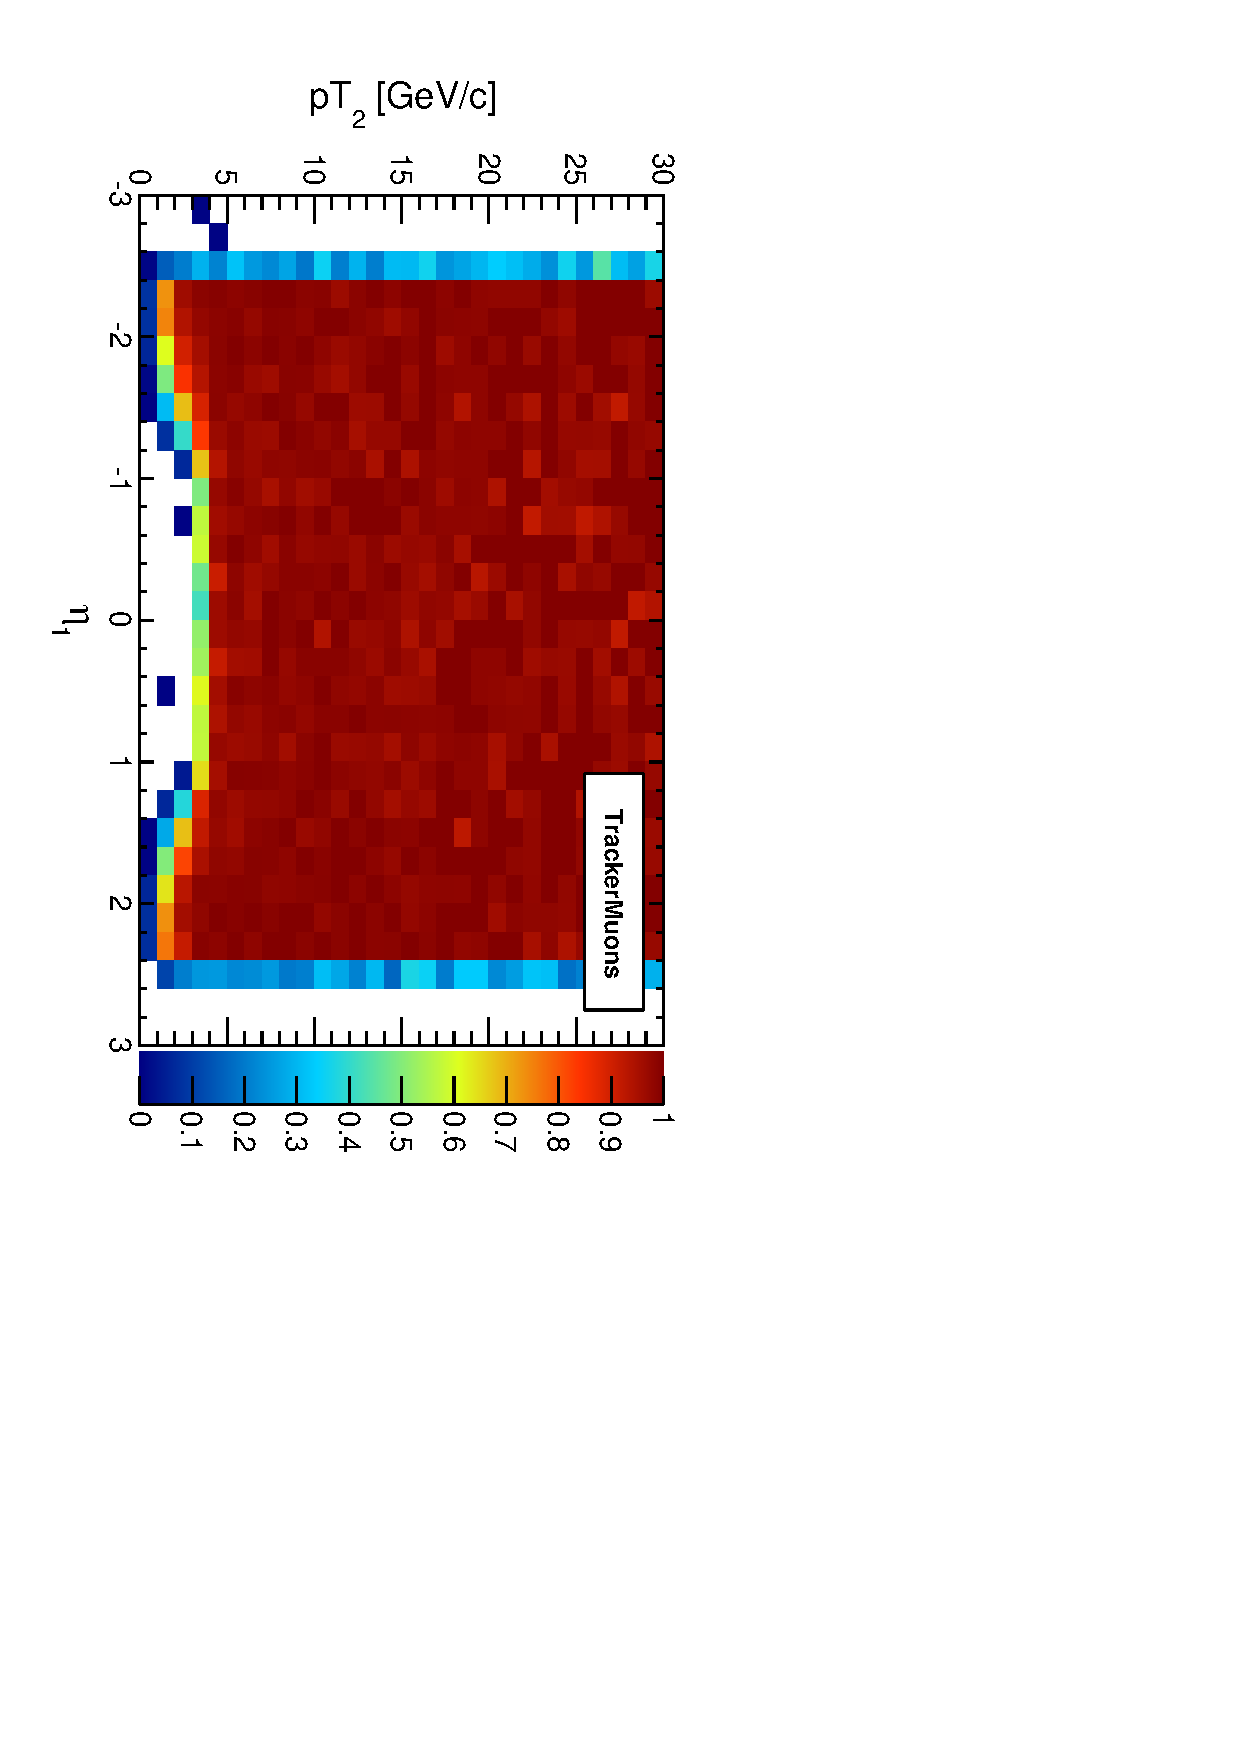
\includegraphics[height=0.45\linewidth, angle=90]{pt2vseta1_TrackerMuons.pdf}
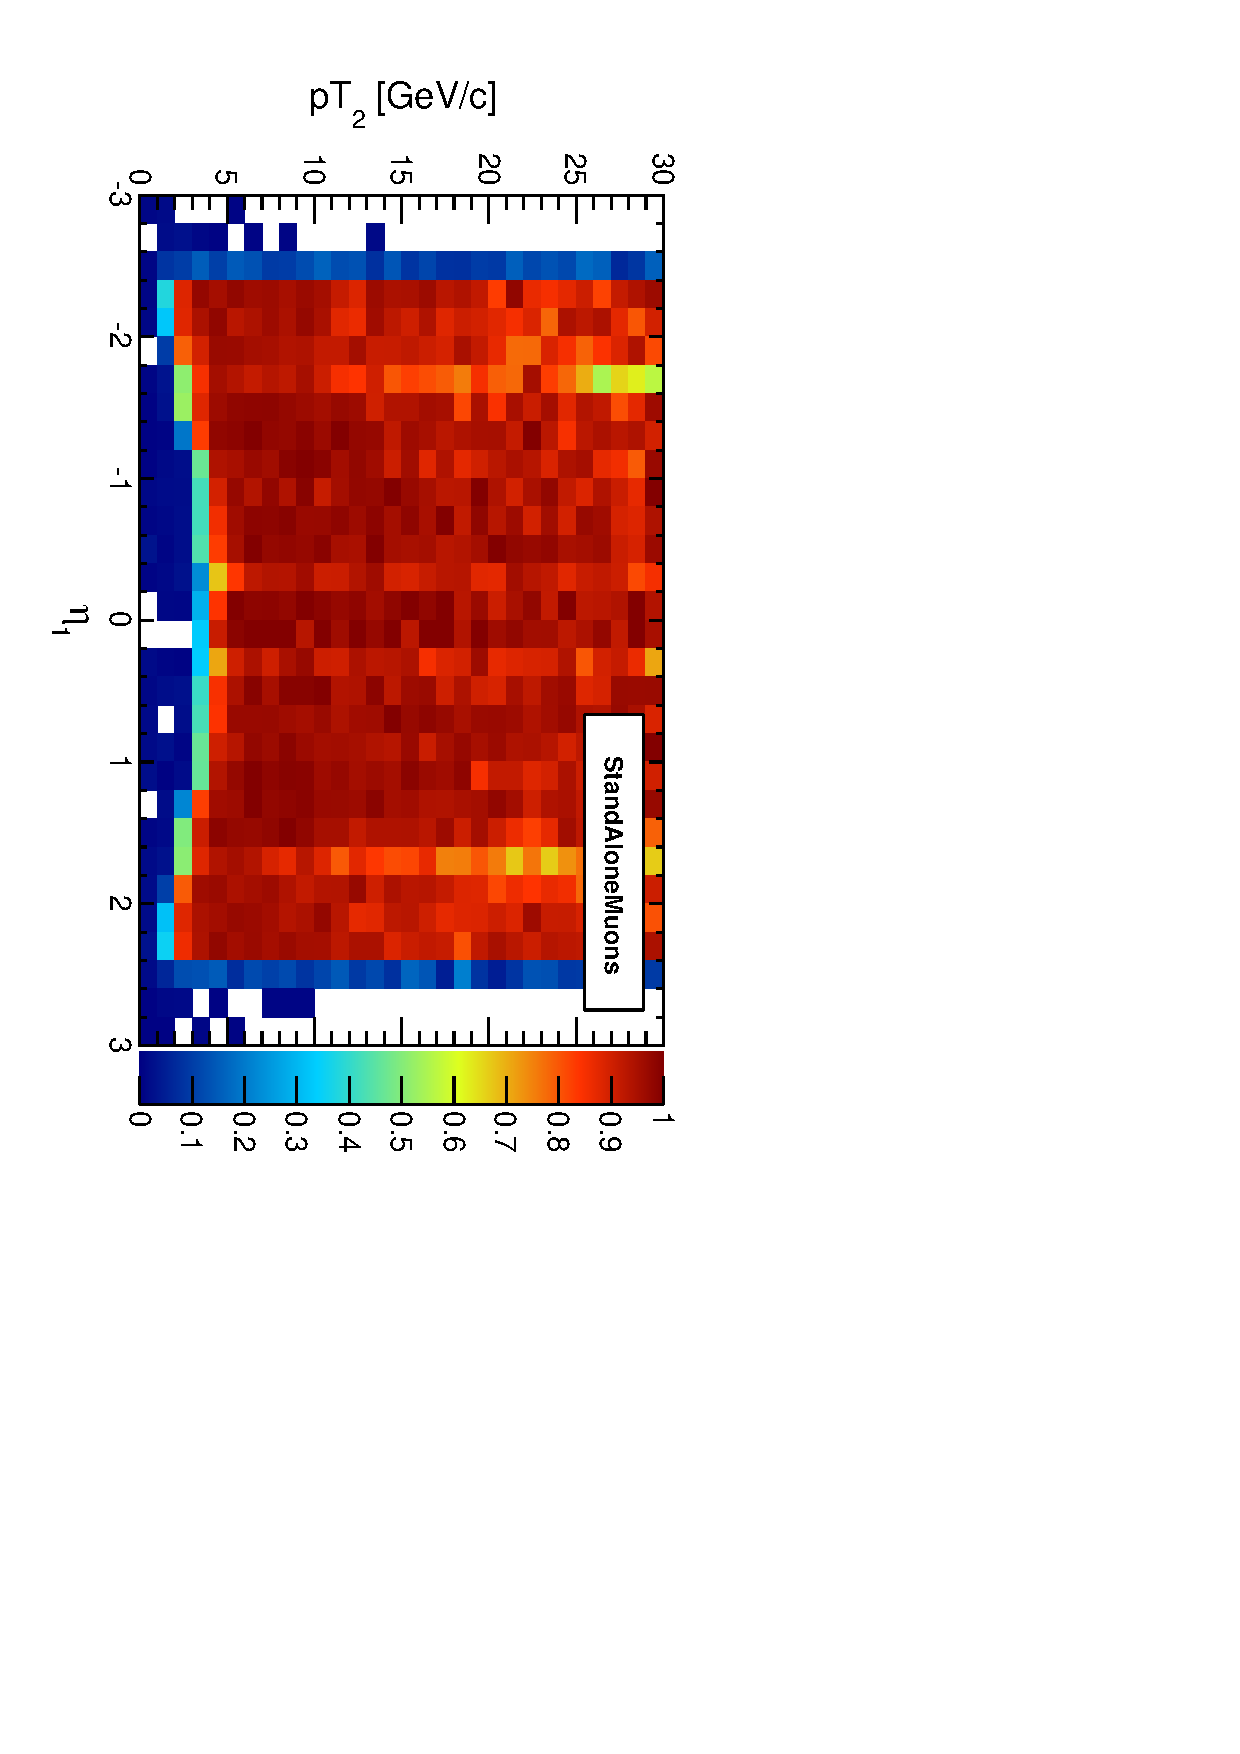
\includegraphics[height=0.45\linewidth, angle=90]{pt2vseta1_StandAloneUpdatedDefault.pdf}

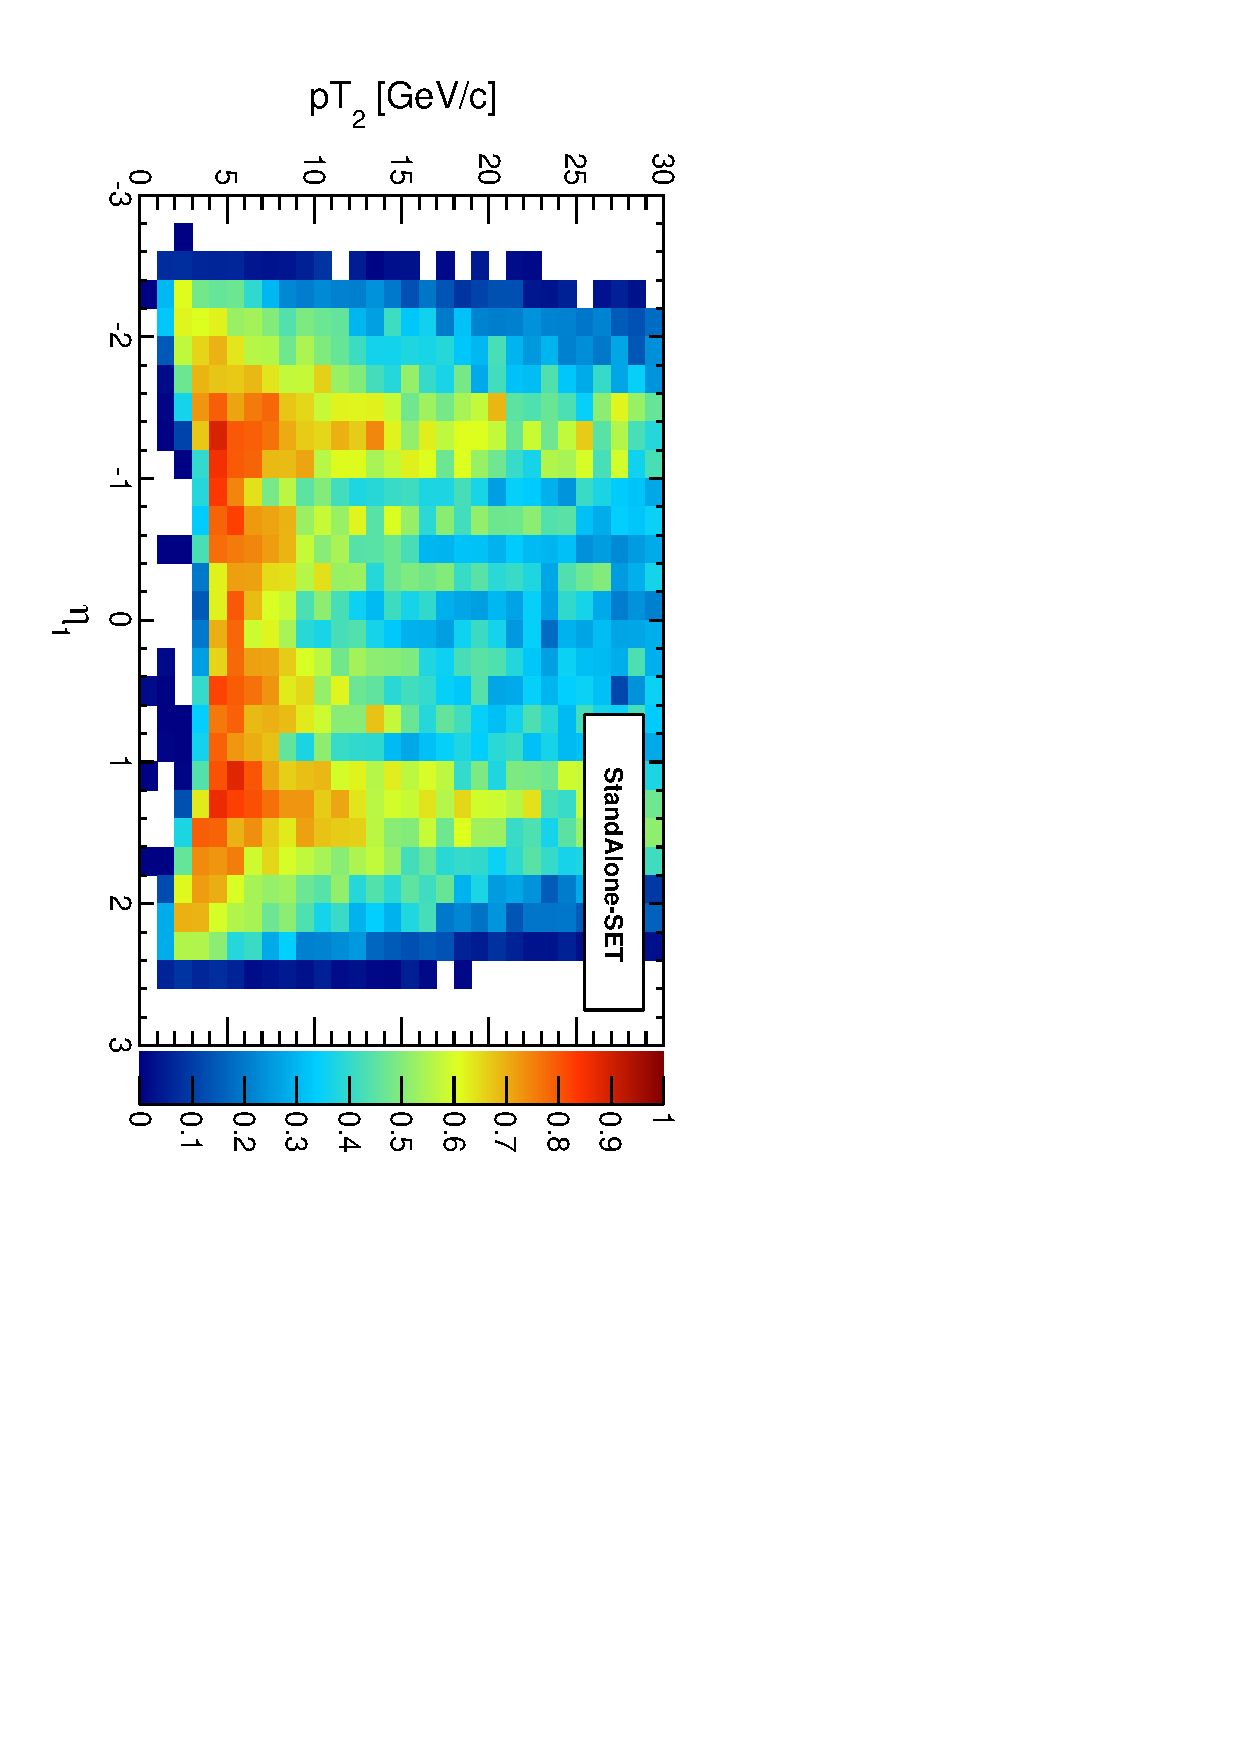
\includegraphics[height=0.45\linewidth, angle=90]{pt2vseta1_StandAloneUpdatedSET.pdf}
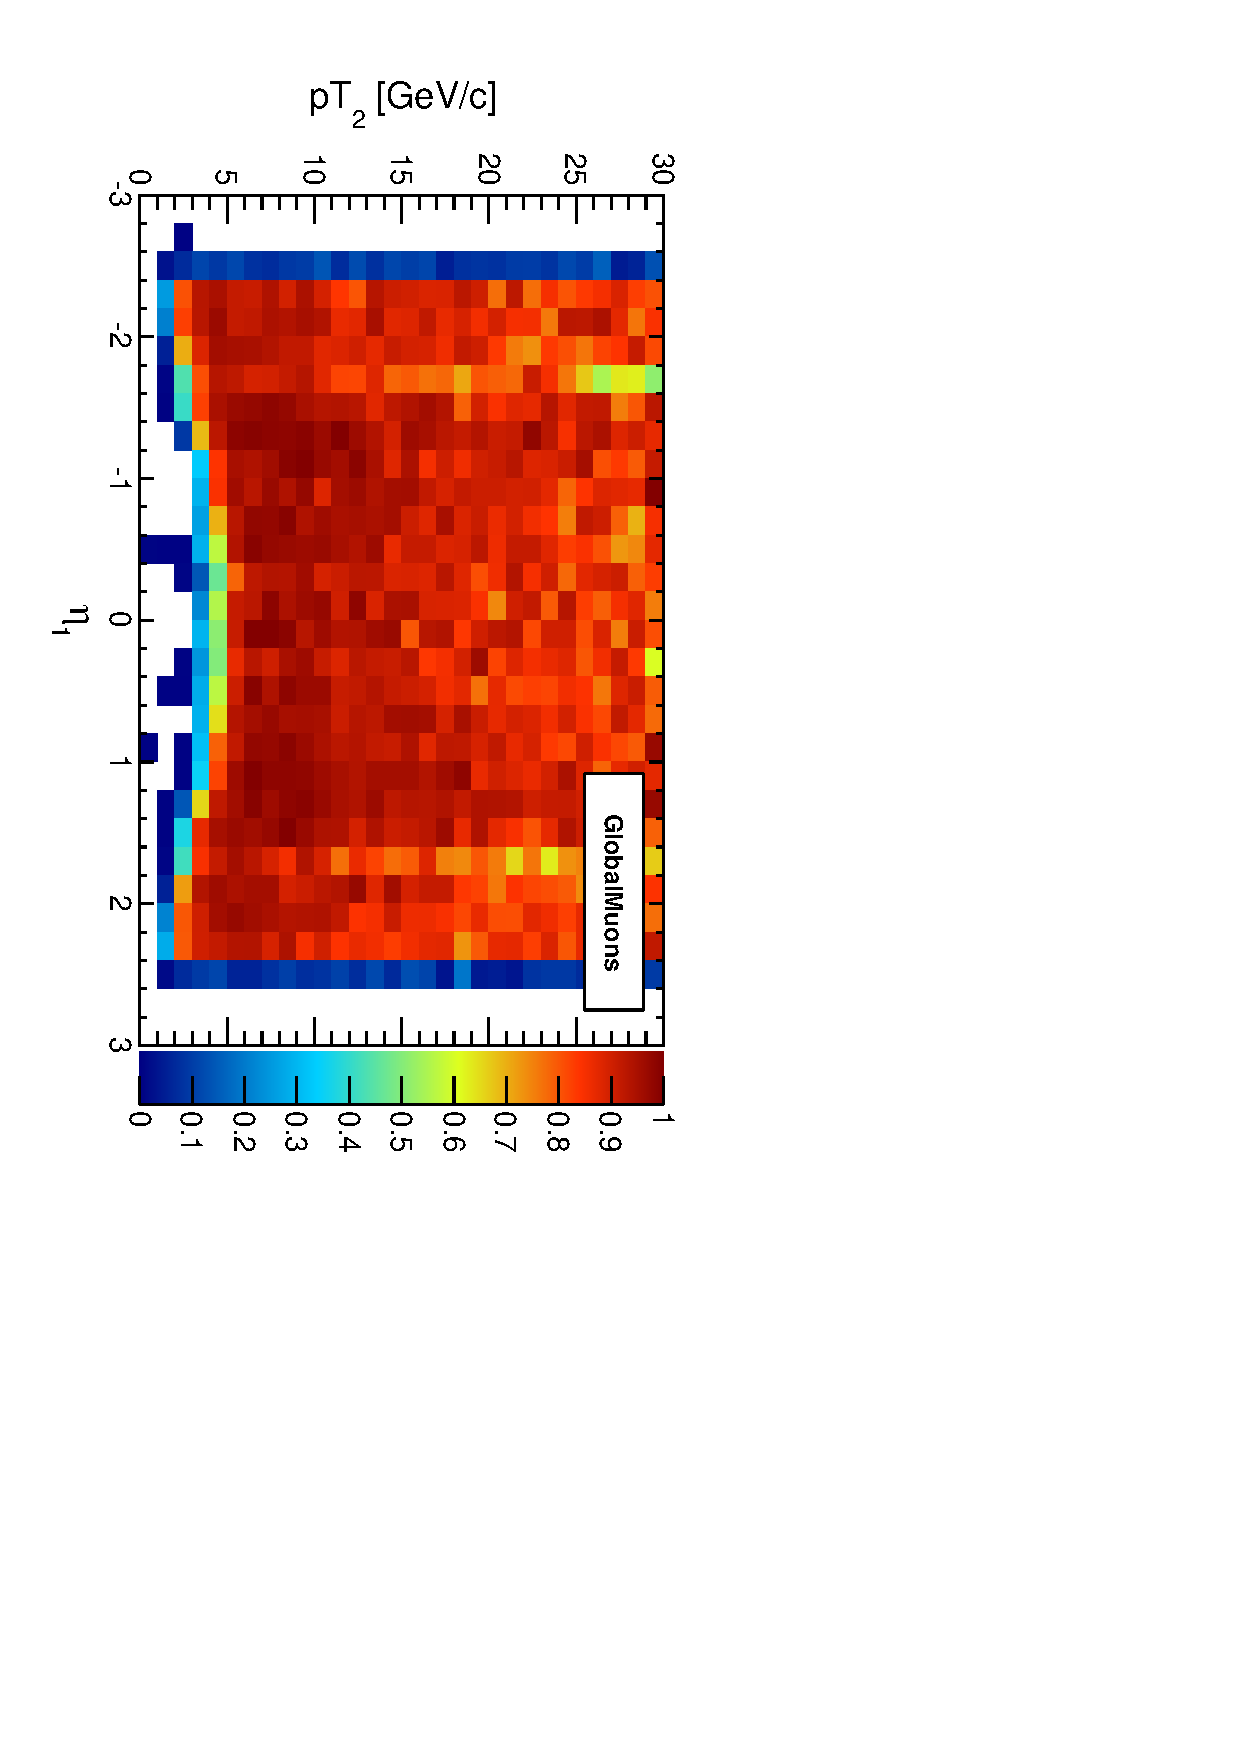
\includegraphics[height=0.45\linewidth, angle=90]{pt2vseta1_GlobalMuons.pdf}
\end{frame}

\begin{frame}
\frametitle{Efficiency plots}
\framesubtitle{Corrections from last time}

\begin{description}
\item[Problem:] efficiency vs.\ crossing in muon system didn't cover a broad range: most interesting parts were low-statistics
\item[Solution:] generated a new muon pair-gun sample with masses uniformly in 0--50~GeV/$c^{2}$, rather than 0--6
\end{description}

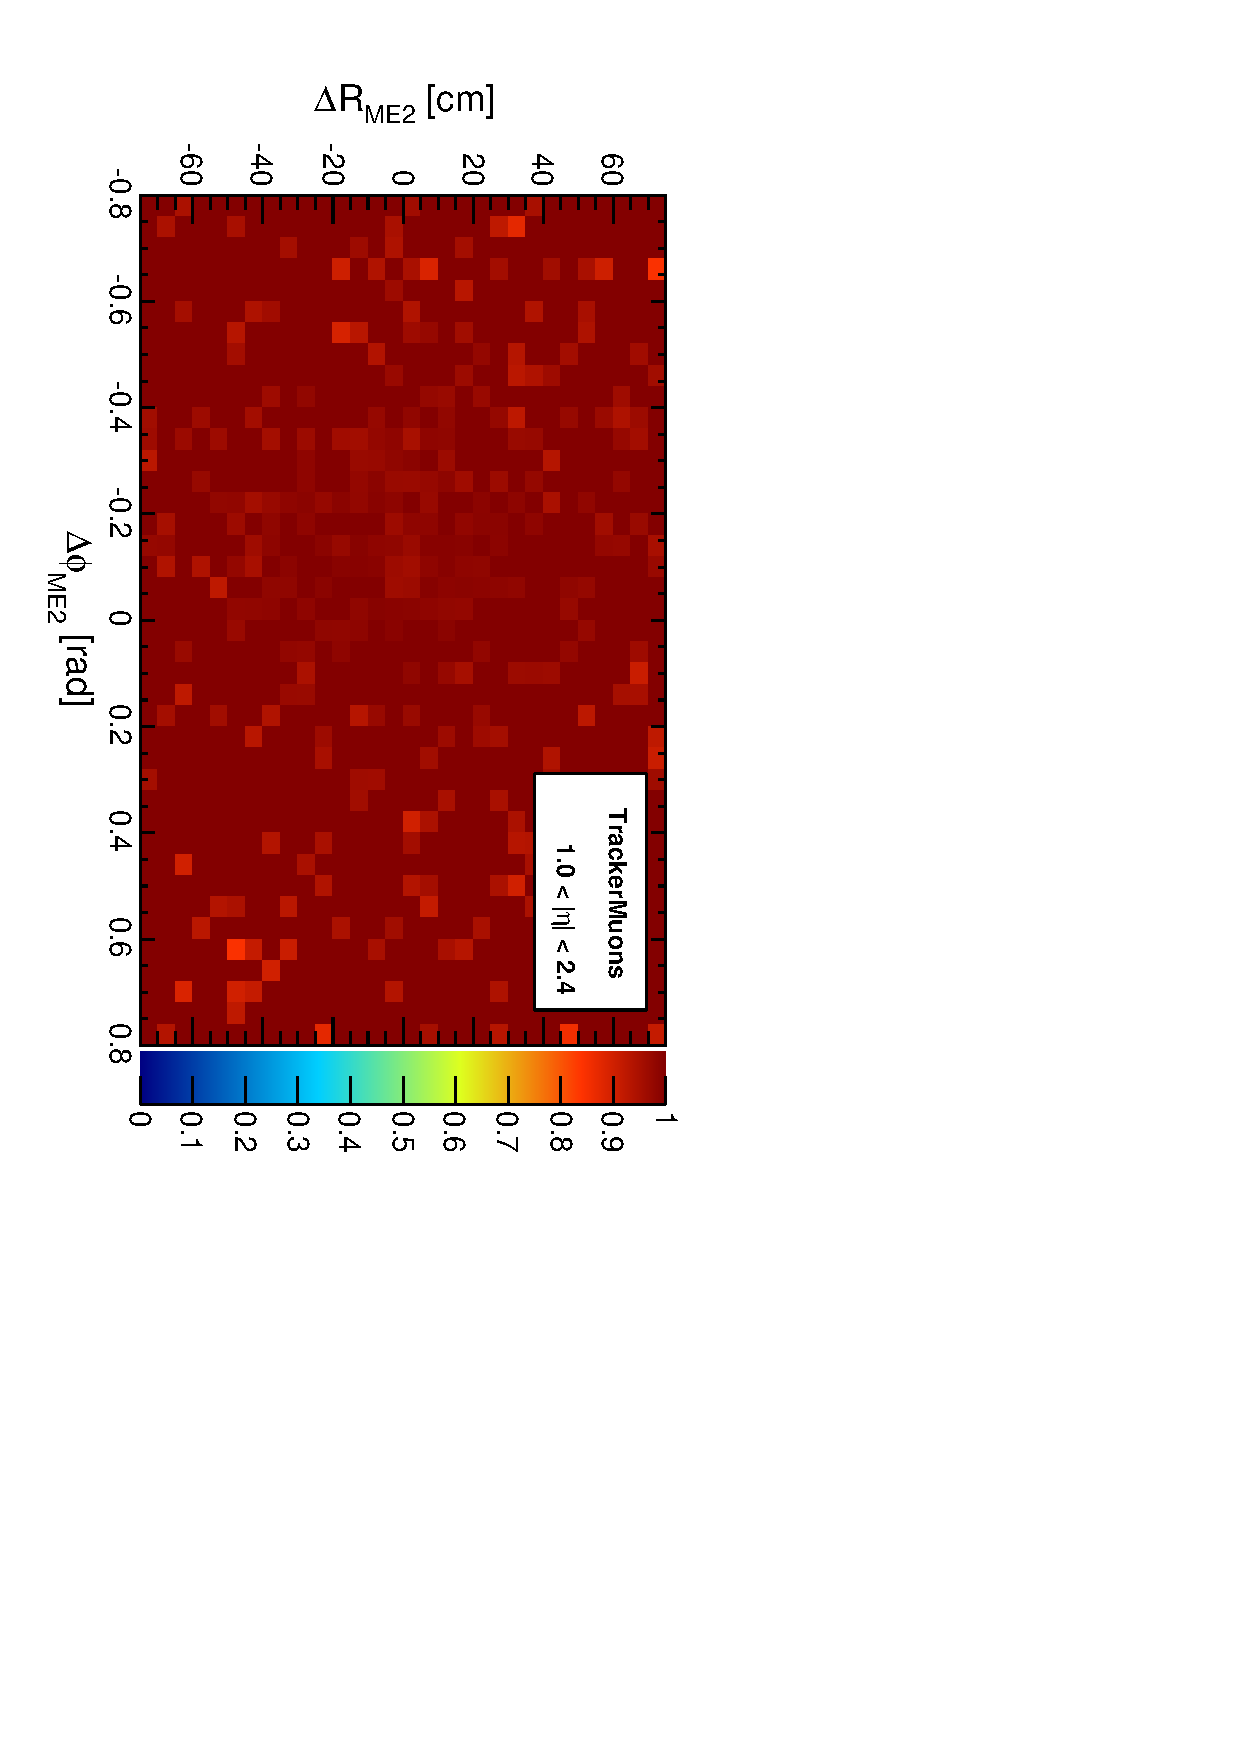
\includegraphics[height=0.45\linewidth, angle=90]{me2_TrackerMuons.pdf}
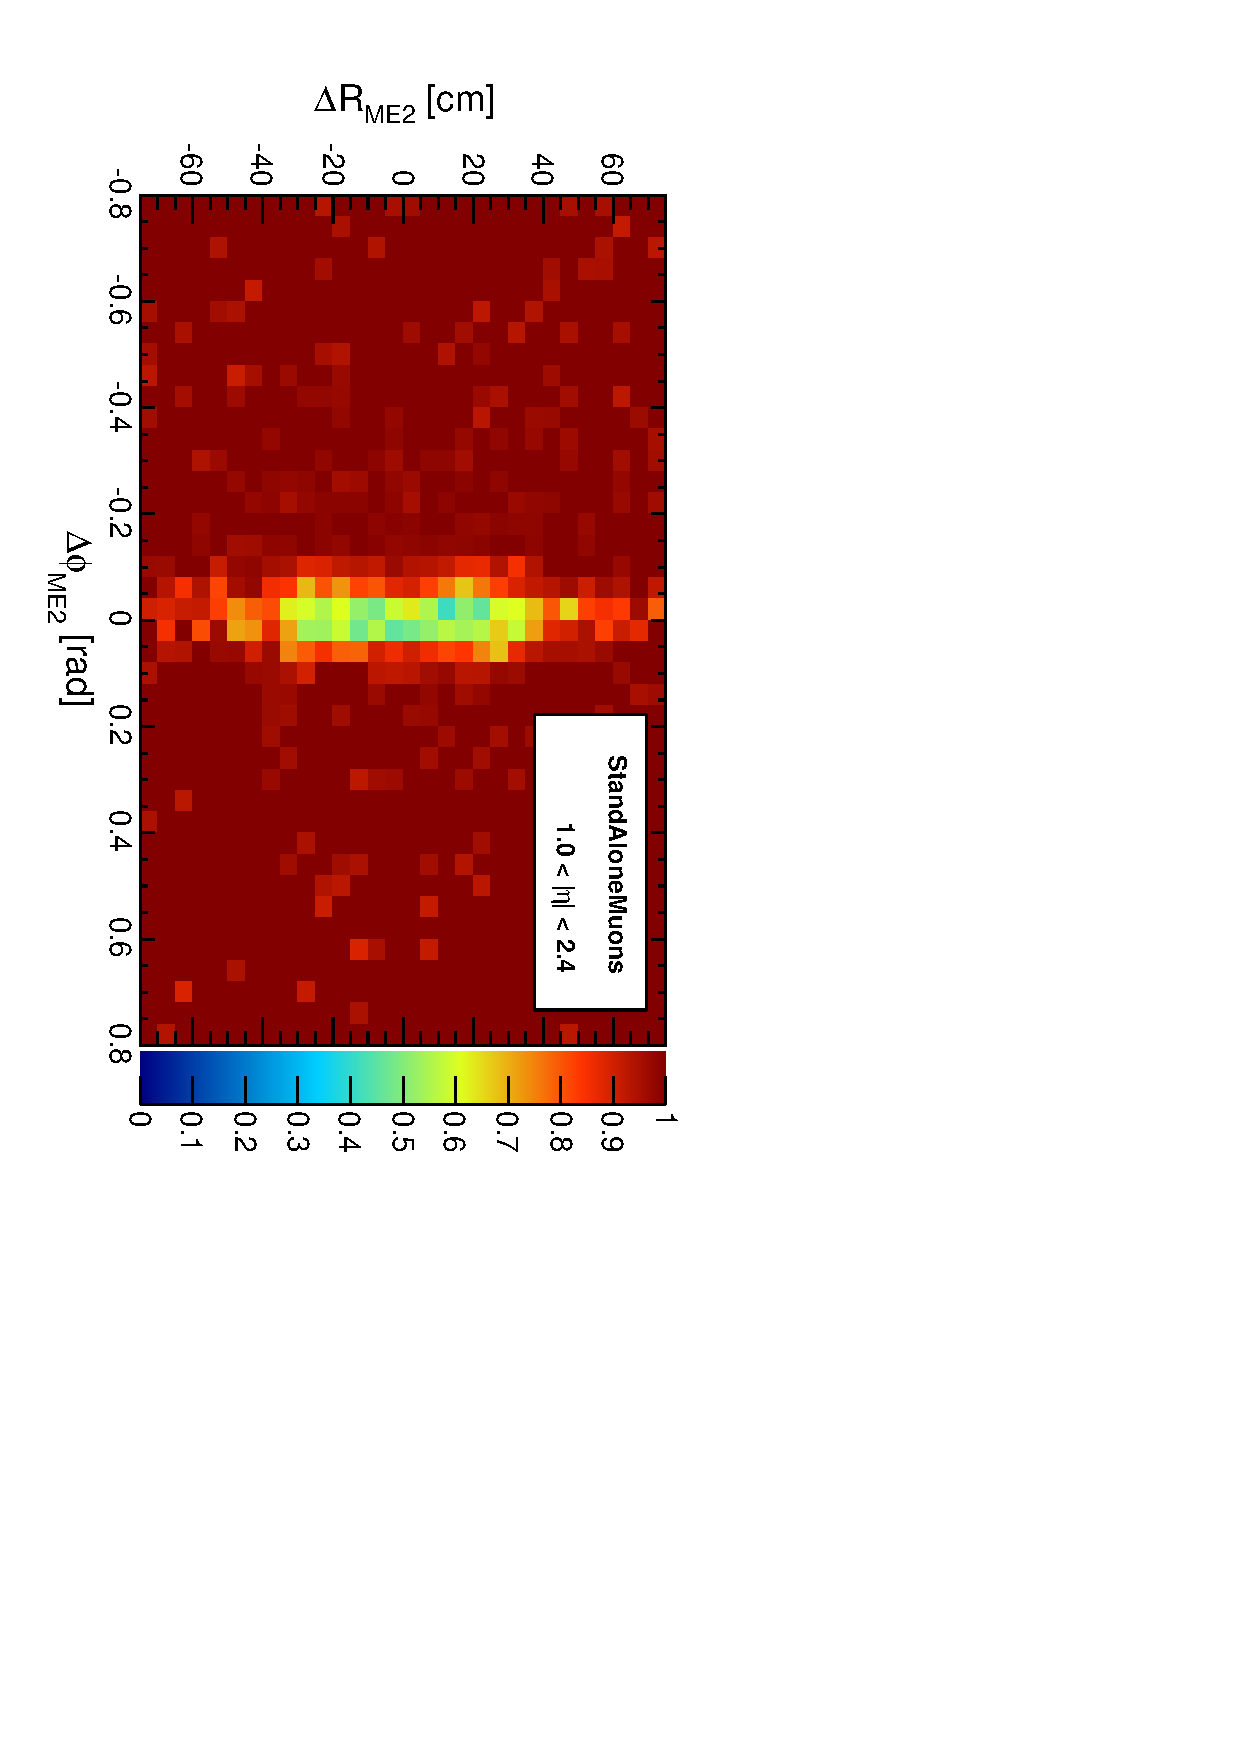
\includegraphics[height=0.45\linewidth, angle=90]{me2_StandAloneUpdatedDefault.pdf}

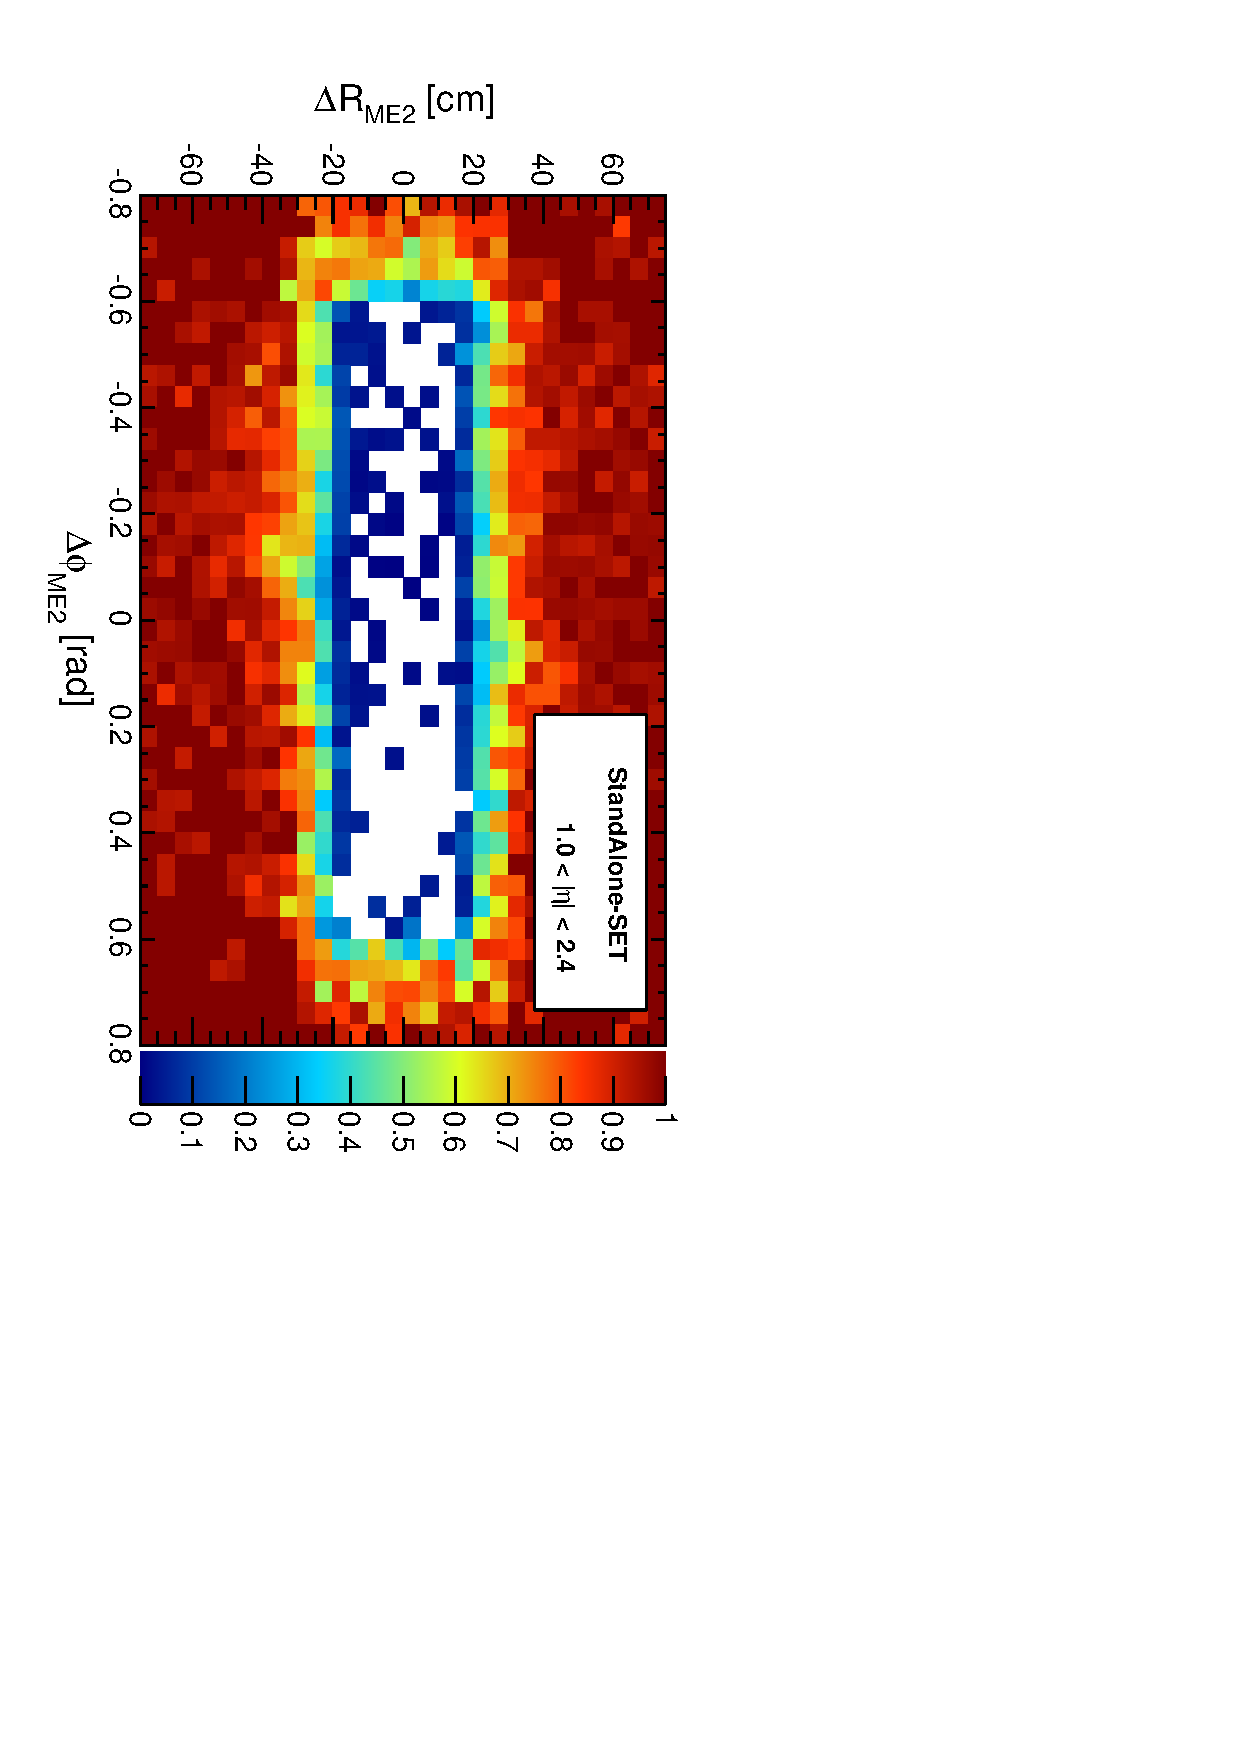
\includegraphics[height=0.45\linewidth, angle=90]{me2_StandAloneUpdatedSET.pdf}
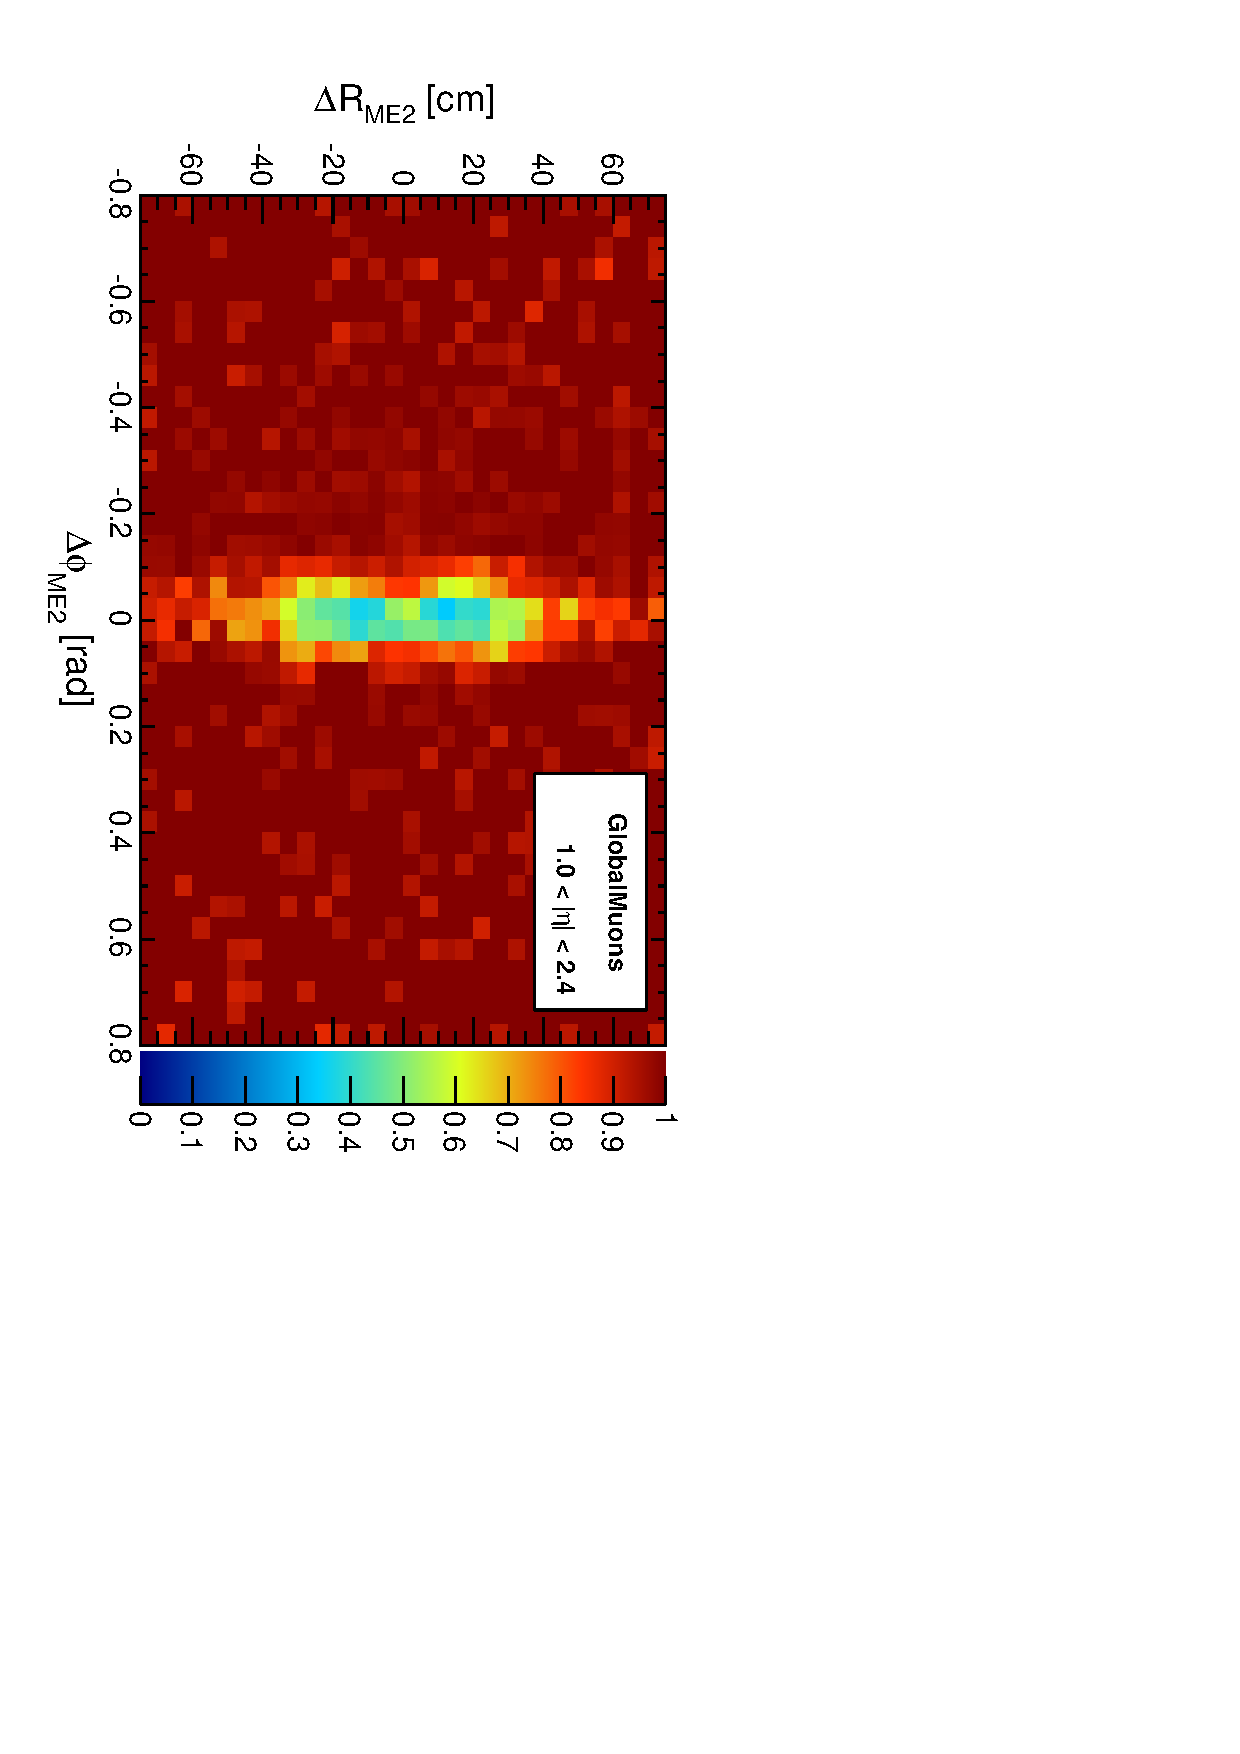
\includegraphics[height=0.45\linewidth, angle=90]{me2_GlobalMuons.pdf}
\end{frame}

\begin{frame}
\frametitle{Efficiency plots}
\framesubtitle{Corrections from last time}

\begin{description}
\item[Remaining problem:] why is inefficiency vs.\ barrel crossing maximal off-center?  Might I be focusing on the wrong place?
\end{description}

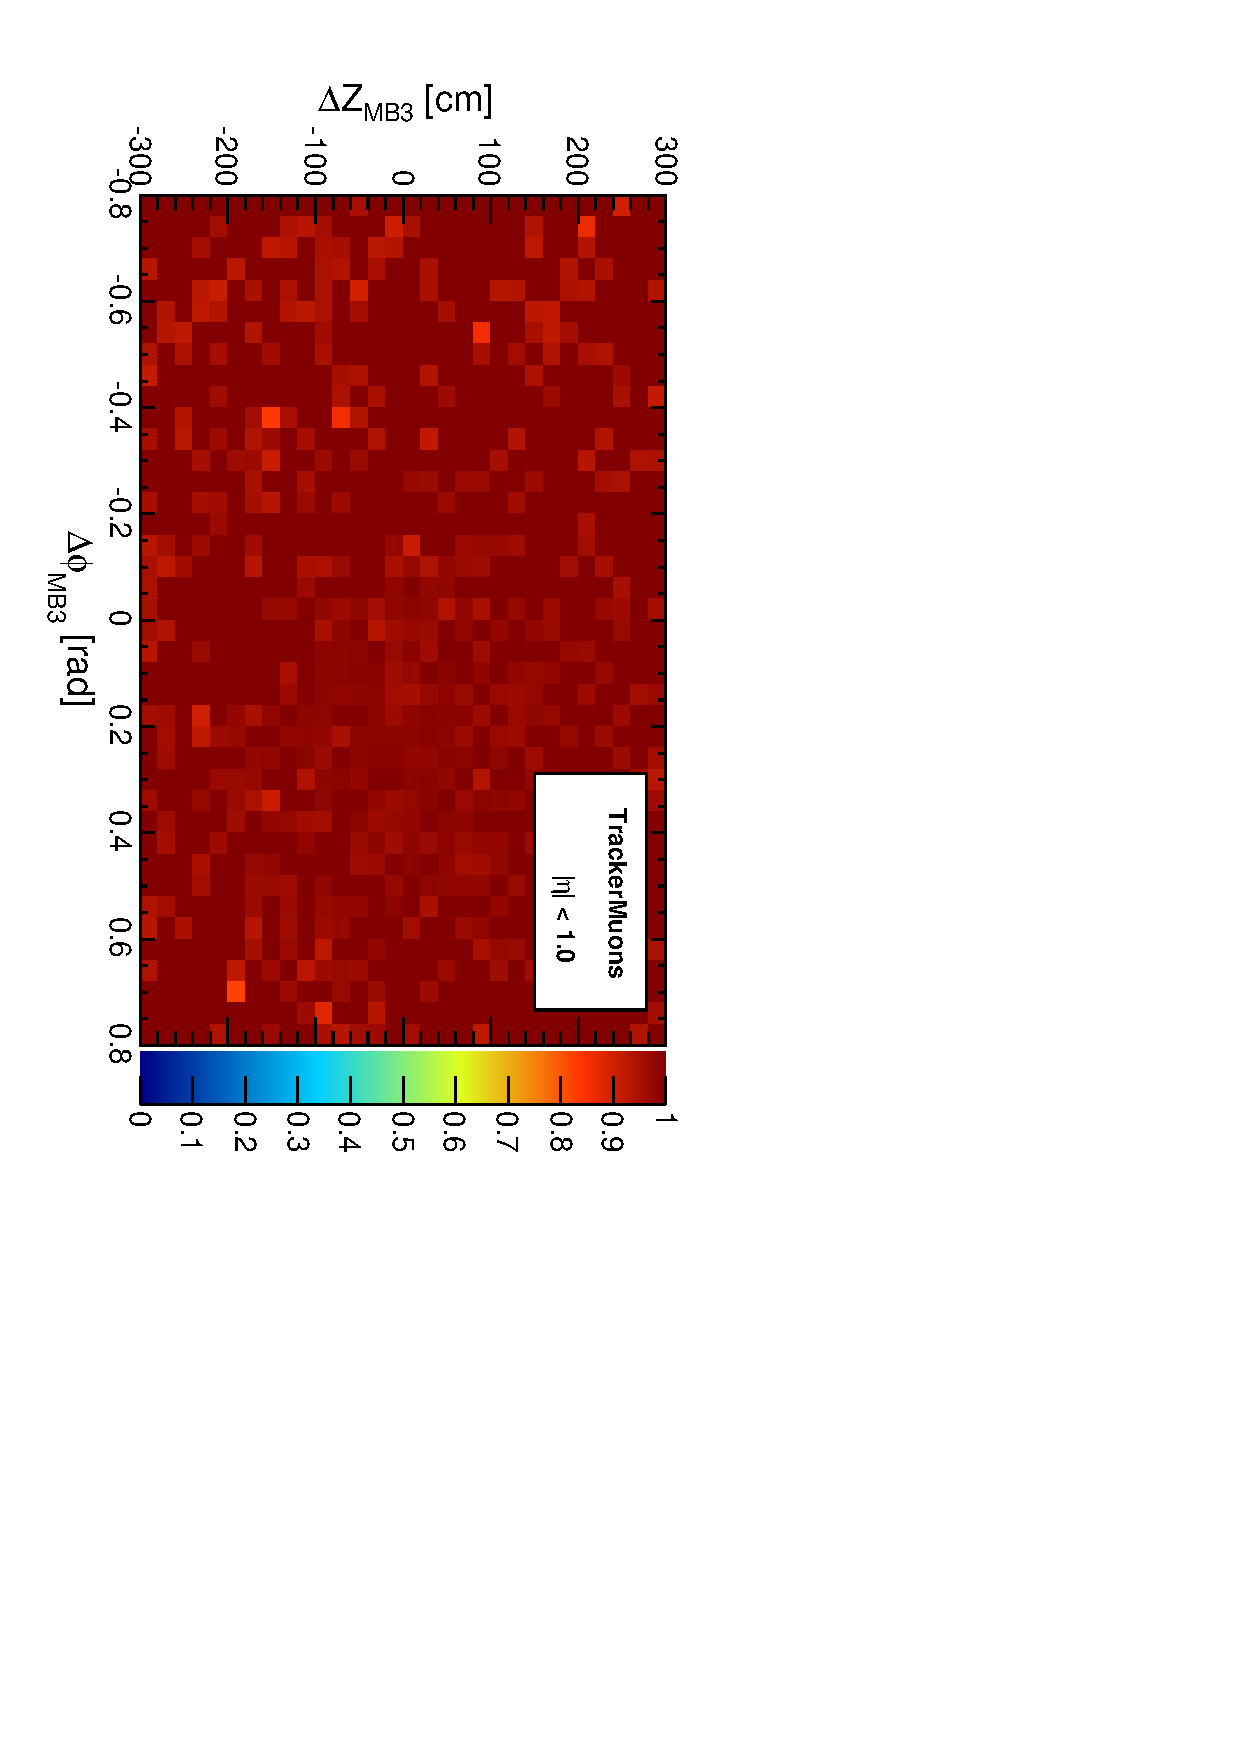
\includegraphics[height=0.45\linewidth, angle=90]{mb3_TrackerMuons.pdf}
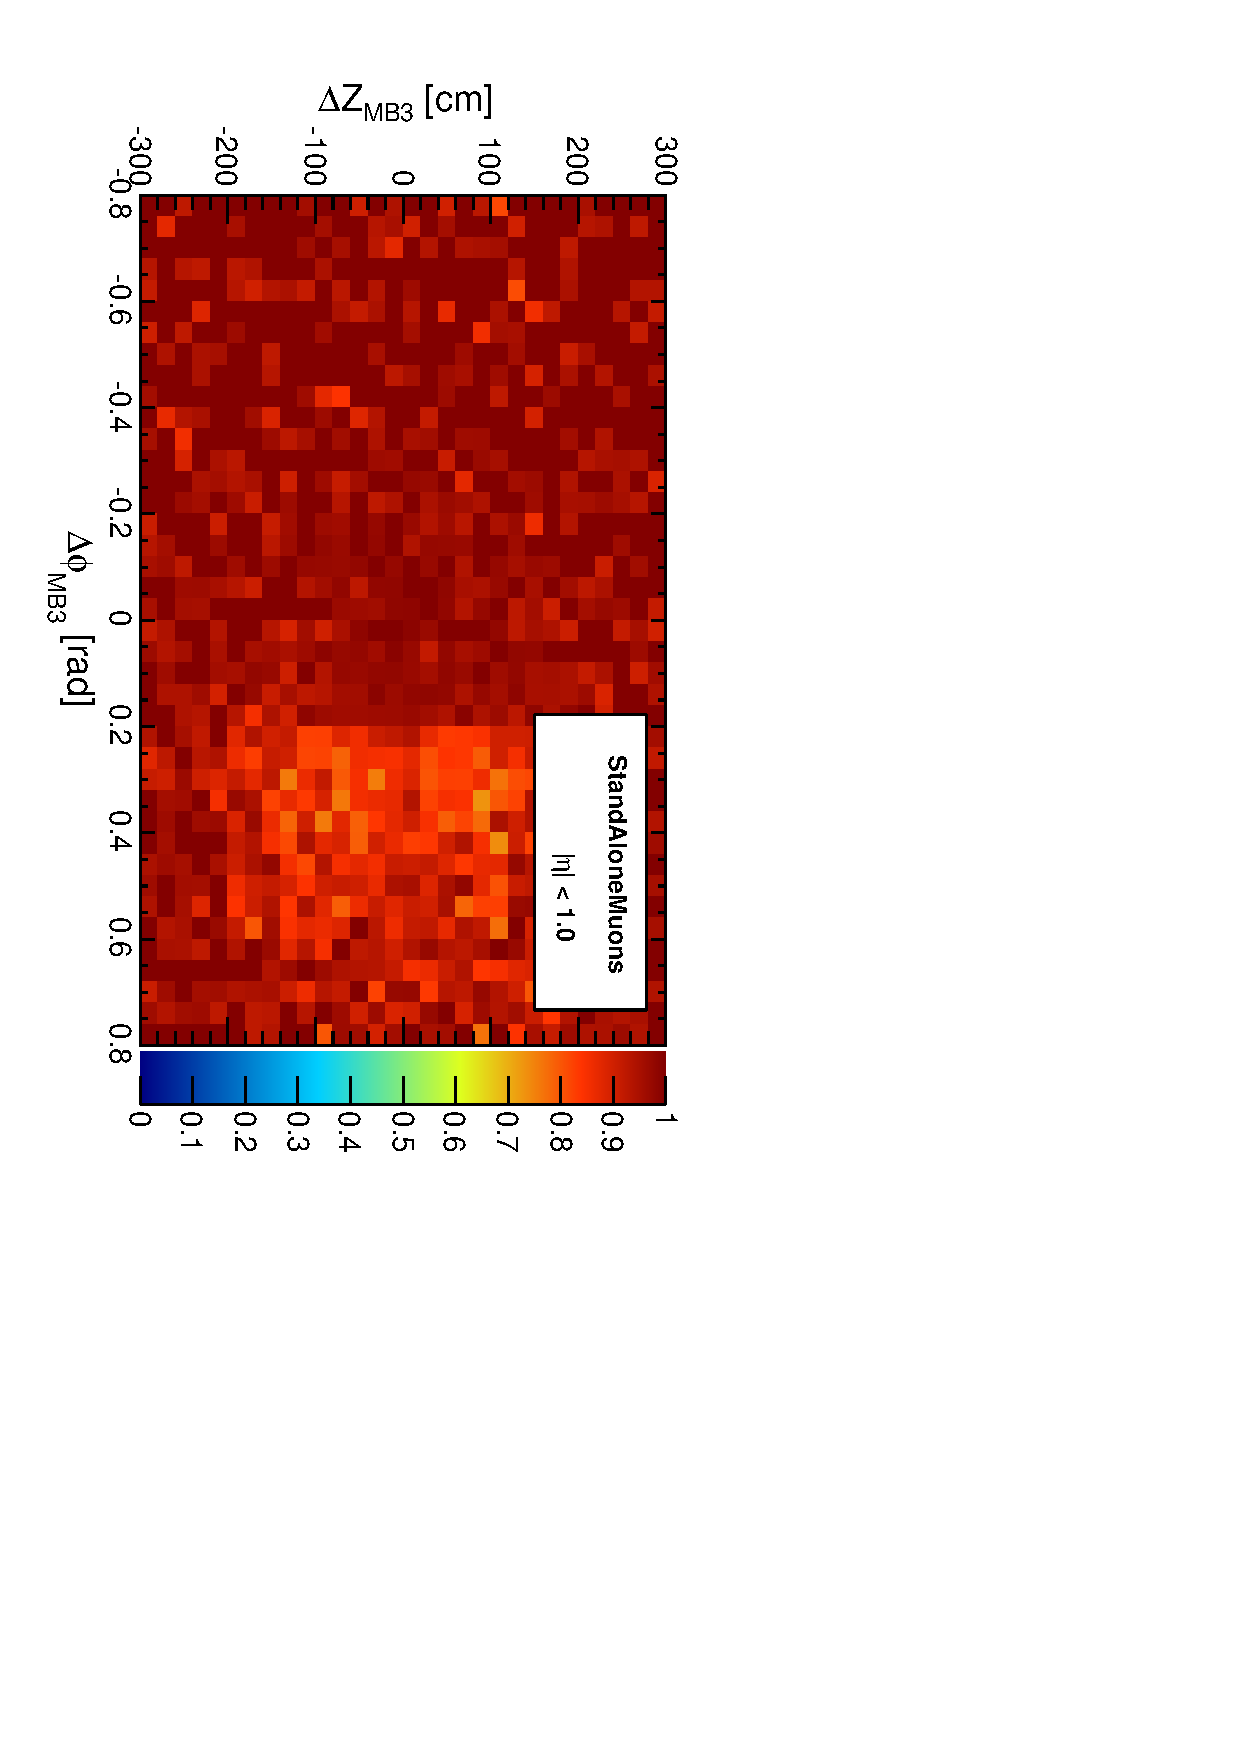
\includegraphics[height=0.45\linewidth, angle=90]{mb3_StandAloneUpdatedDefault.pdf}

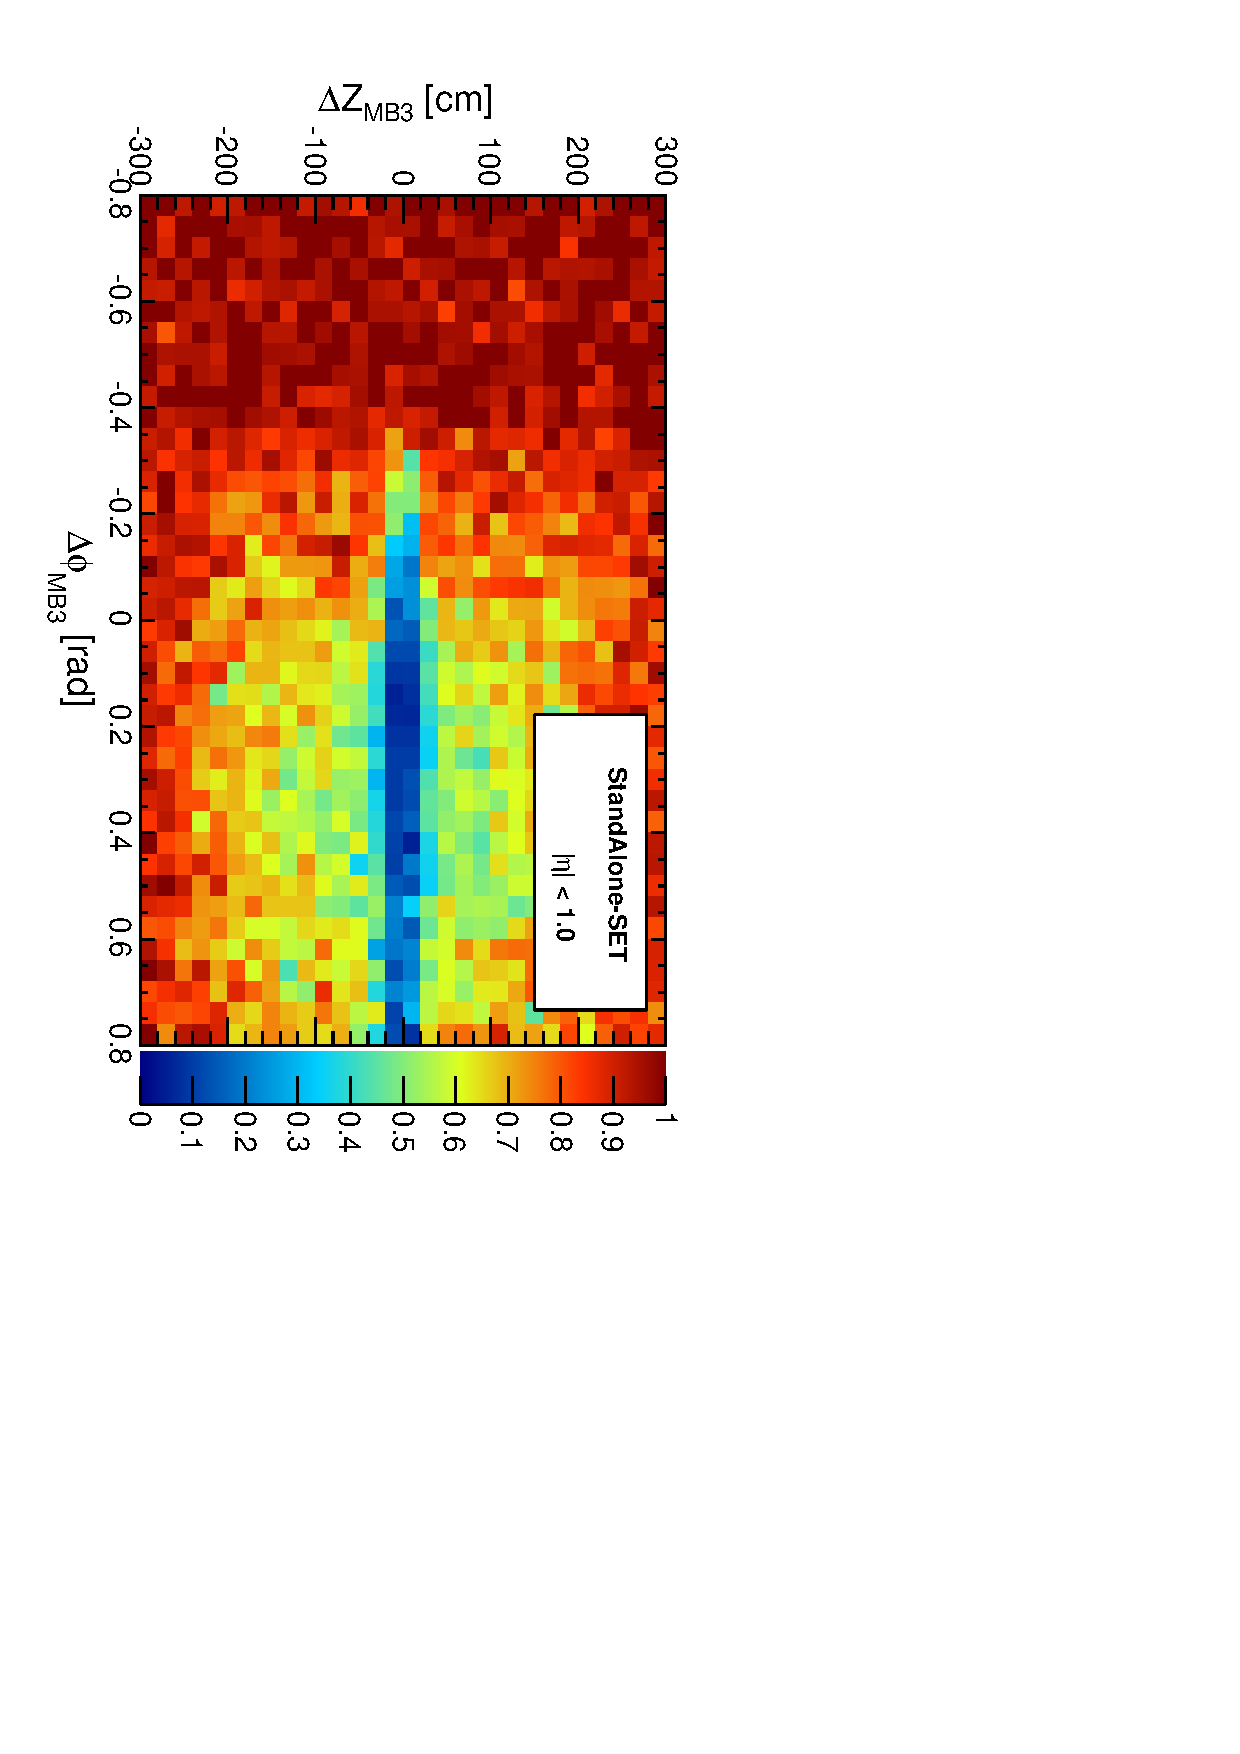
\includegraphics[height=0.45\linewidth, angle=90]{mb3_StandAloneUpdatedSET.pdf}
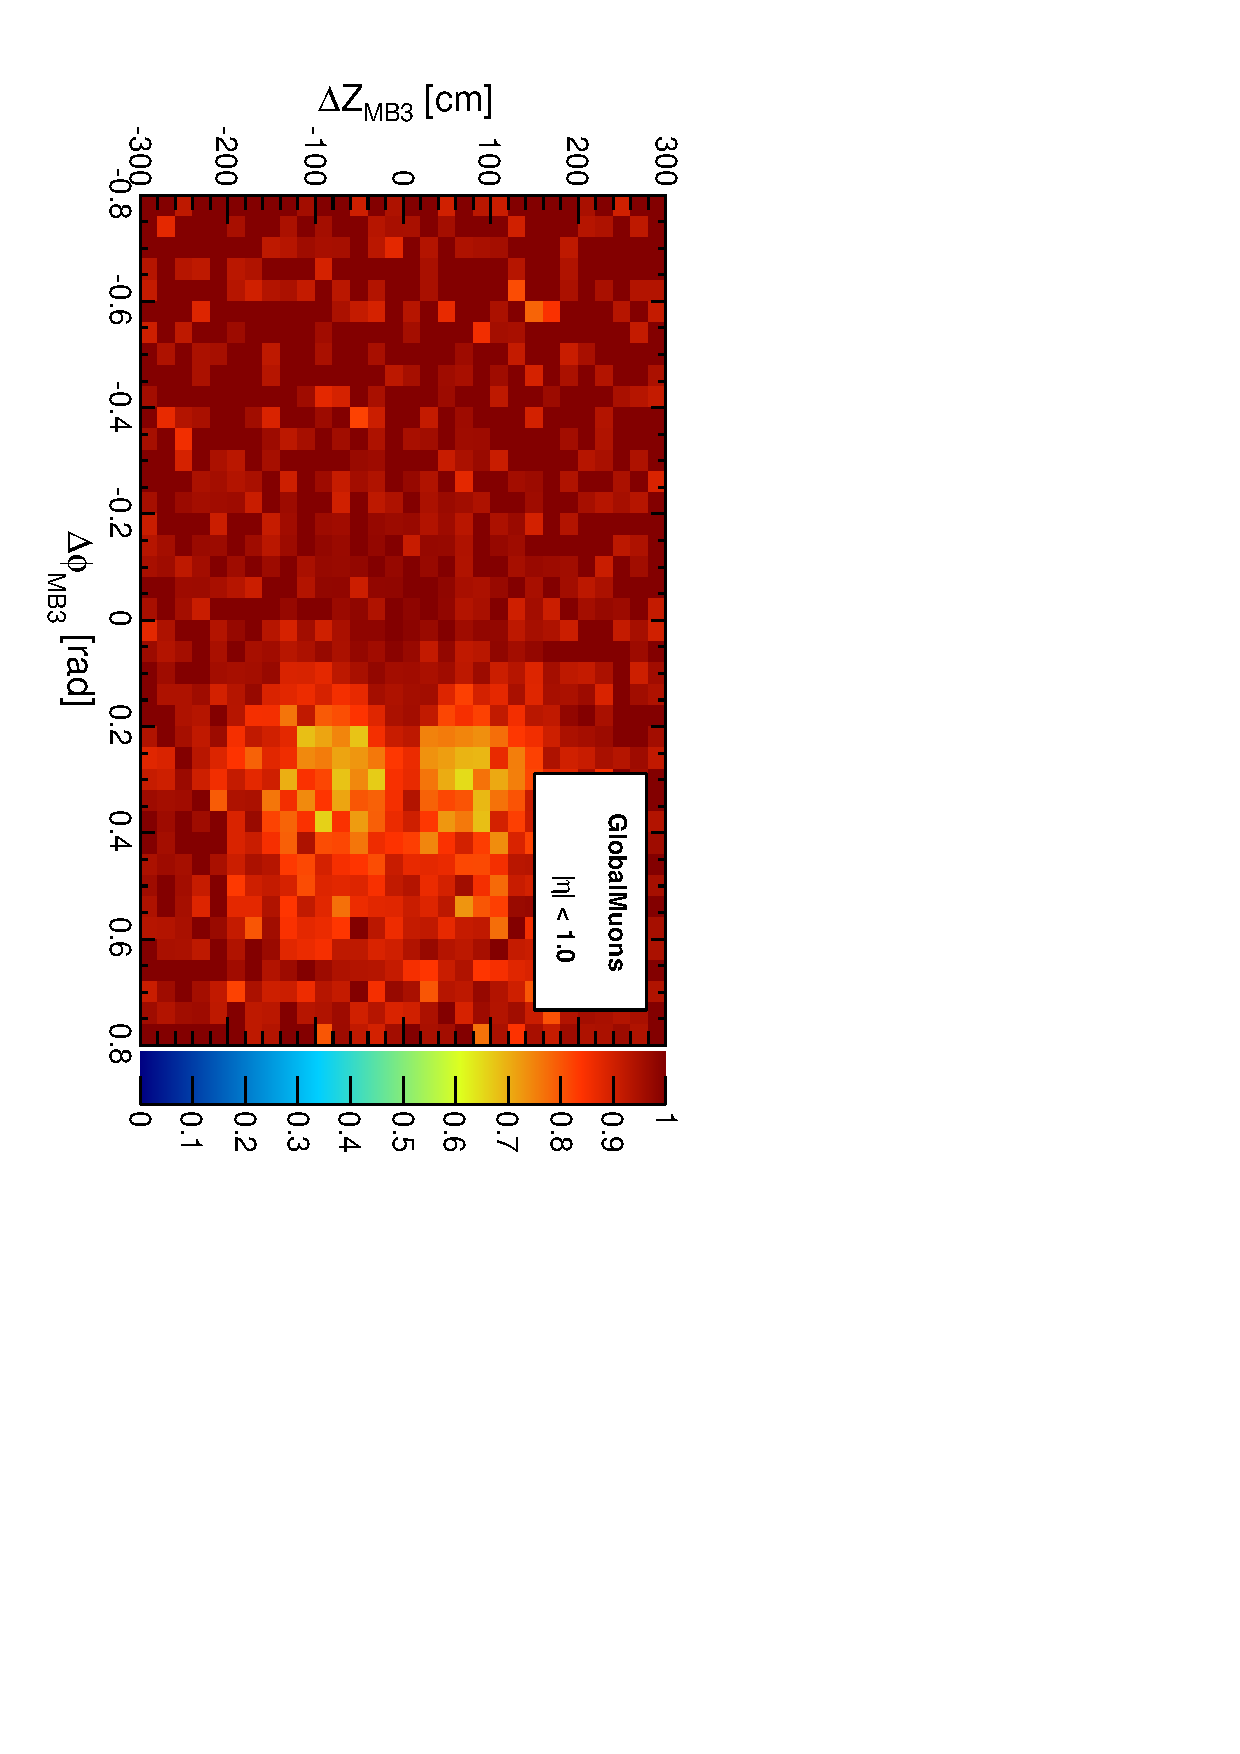
\includegraphics[height=0.45\linewidth, angle=90]{mb3_GlobalMuons.pdf}
\end{frame}

\begin{frame}
\frametitle{Efficiency plots}
\framesubtitle{The requested ``denominator'' plots}

\begin{itemize}
\item These are distributions of where you would land in the muon system if you had dimuons uniformly distributed in mass, 0--6~GeV/$c^{2}$, uniform in $p_T$, 0--100~GeV/$c$, uniform in $\eta$, decaying like a scalar (``spherically'')
\item A different model would have a different distribution (which is why it would be useful to avoid GlobalMuons, so that the efficiency doesn't depend on the kinematics in a complicated way).
\end{itemize}

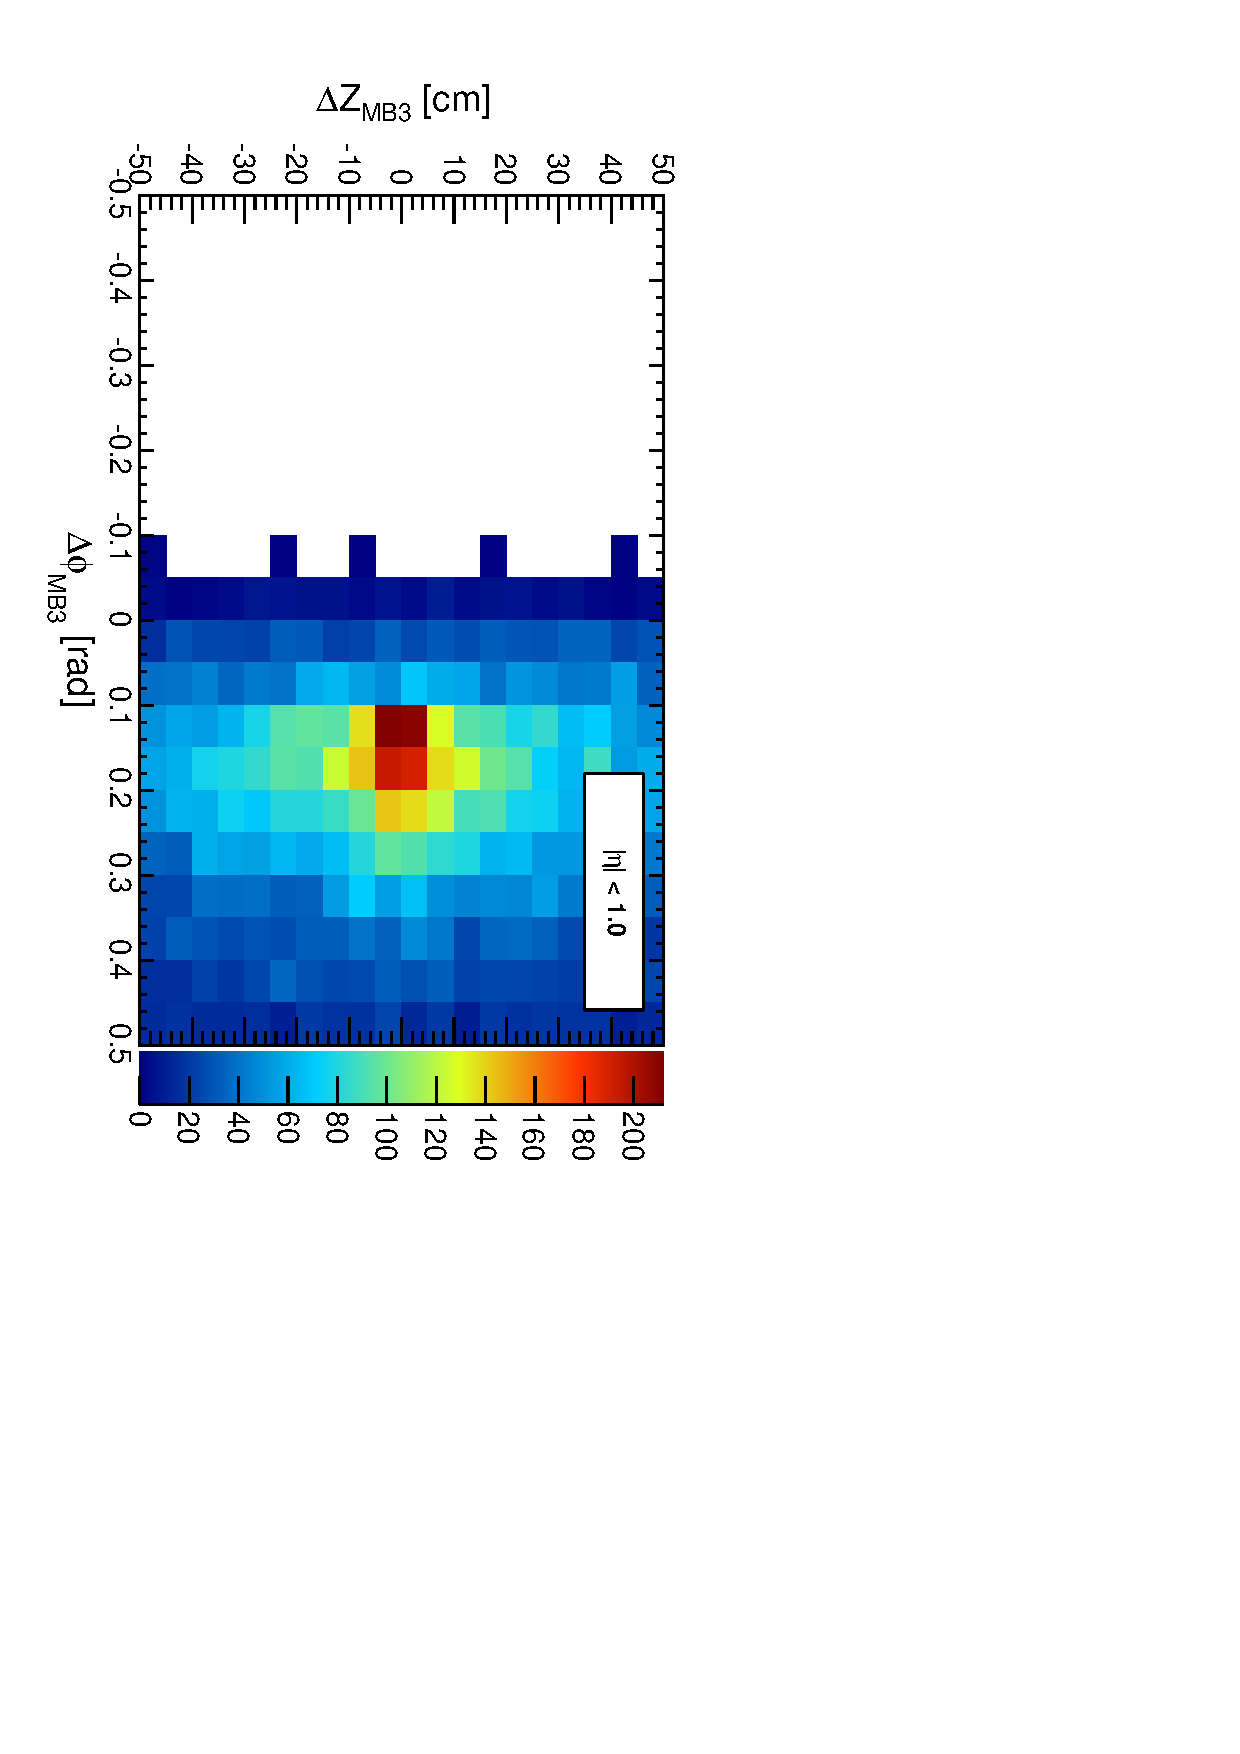
\includegraphics[height=0.5\linewidth, angle=90]{mb3_TrackerMuons_denominator.pdf}
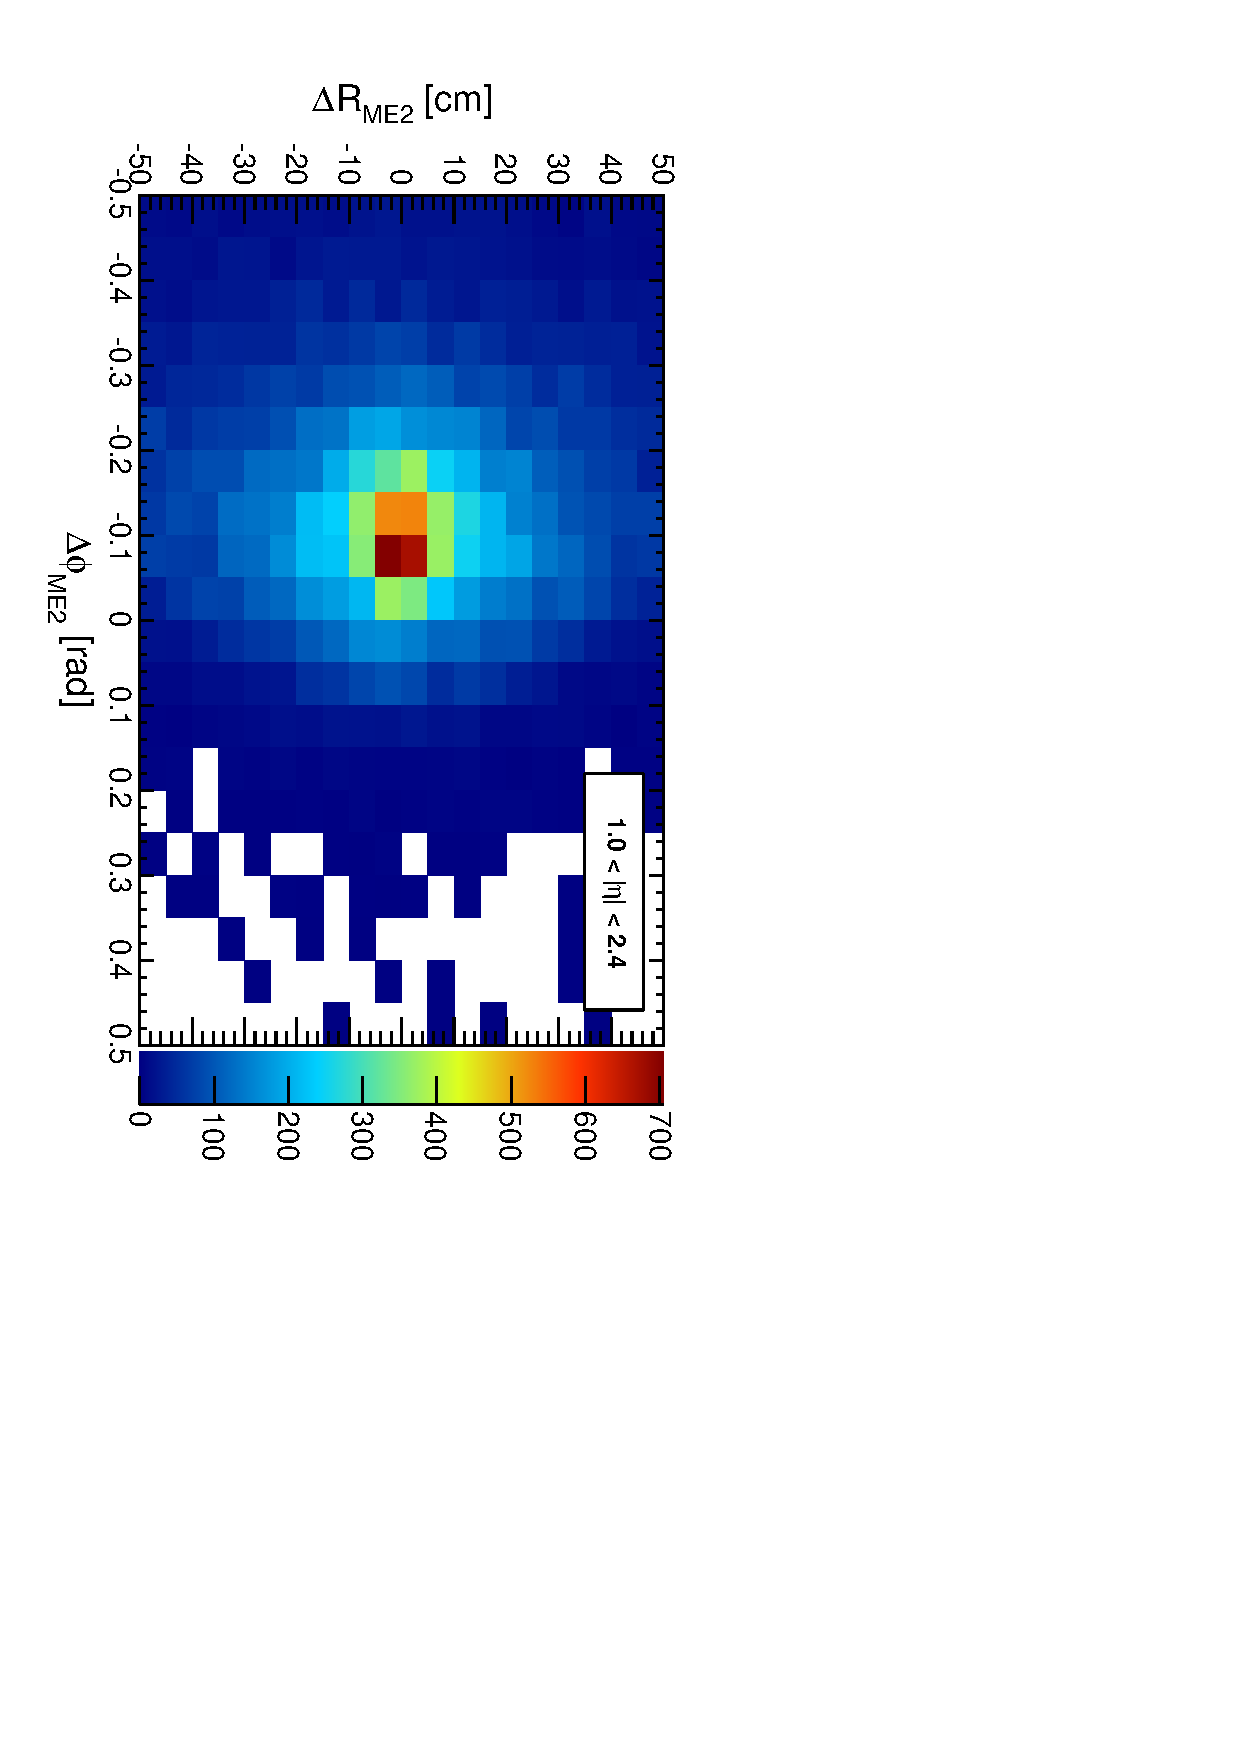
\includegraphics[height=0.5\linewidth, angle=90]{me2_TrackerMuons_denominator.pdf}
\end{frame}

\begin{frame}
\frametitle{Efficiency plots}
\framesubtitle{Same in profile}

\begin{itemize}
\item Trying a new technique: every muon in the dimuon-gun sample is also simulated and reconstructed in its own individual event, so that we can see the efficiency of all muons together and the efficiency of each muon separately
\item We don't need to worry about regions in which $\epsilon_{\mu^+\mu^-} = \epsilon_{\mu^+} \times \epsilon_{\mu^-}$
\end{itemize}

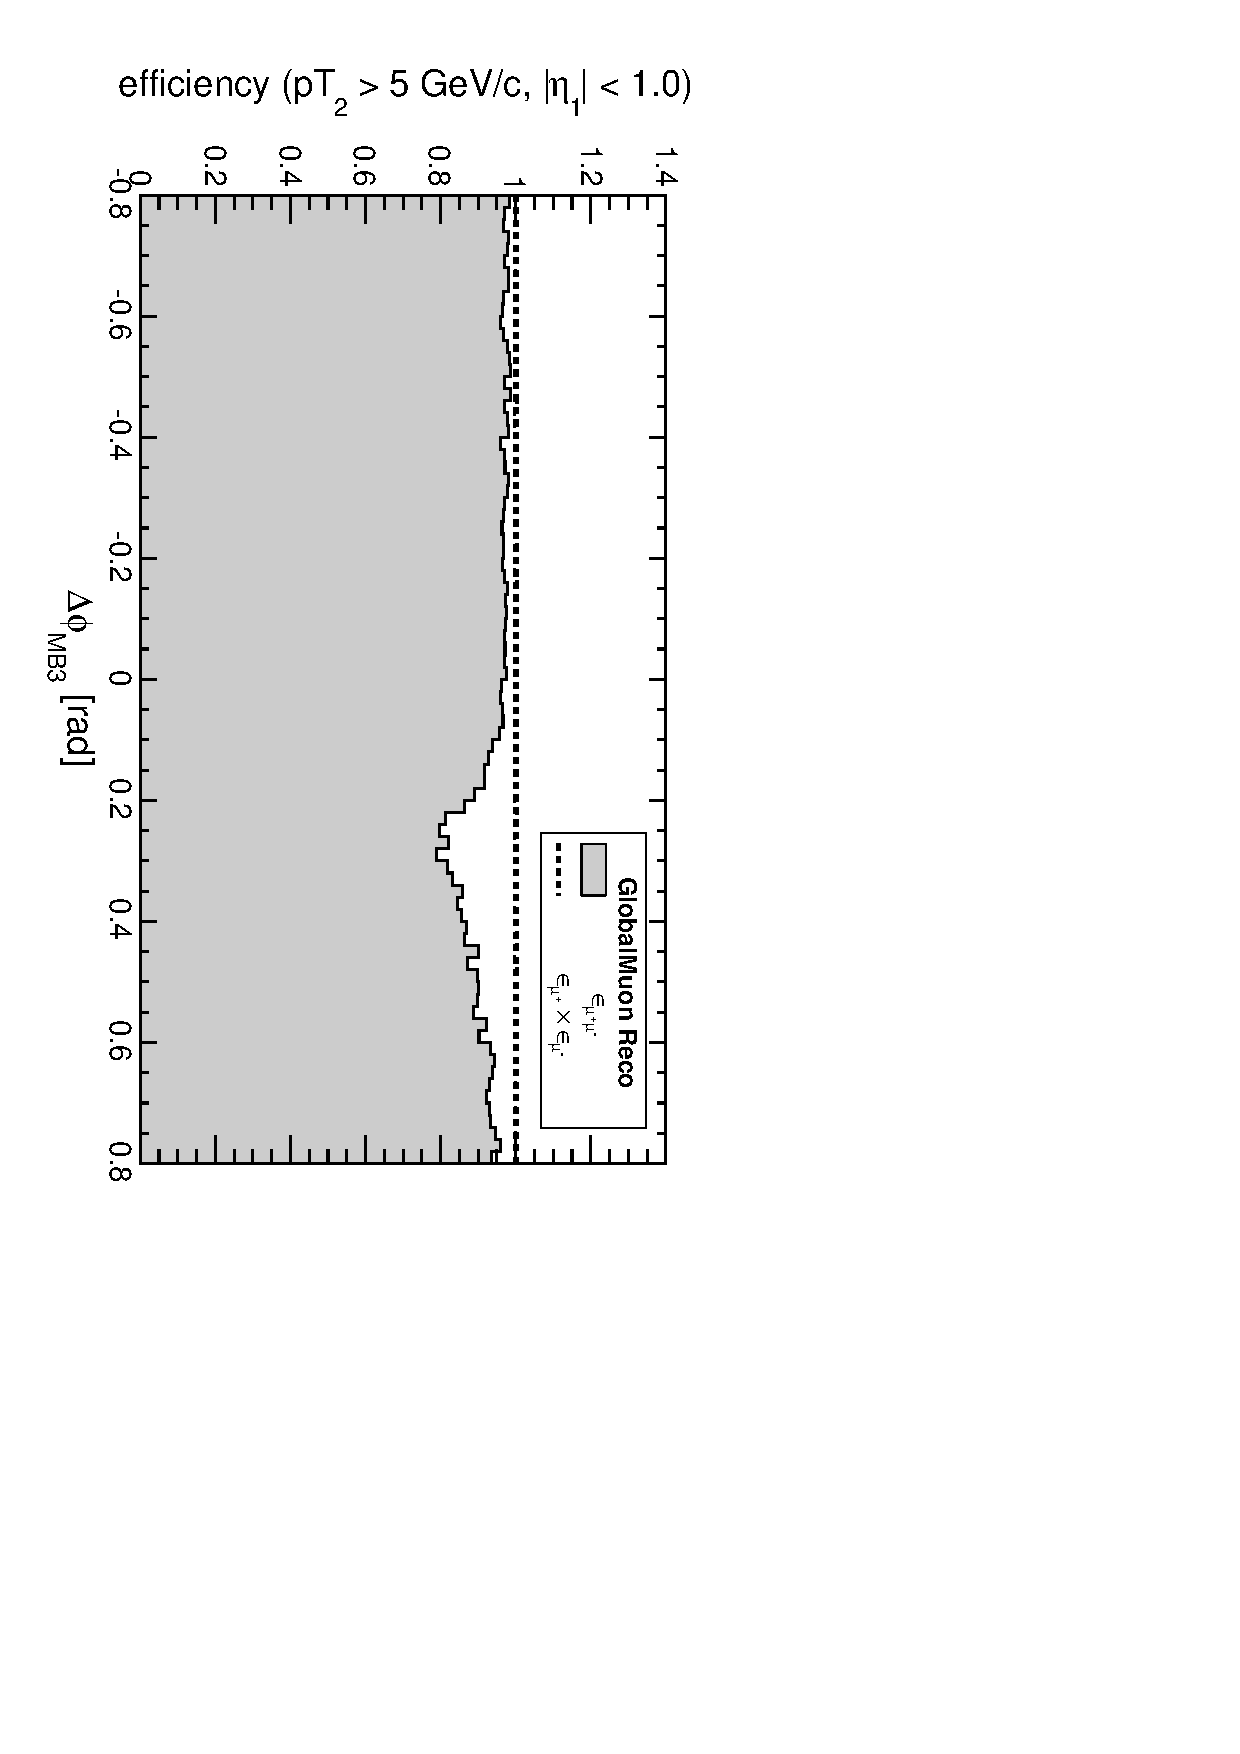
\includegraphics[height=0.45\linewidth, angle=90]{vsmb3dphi_GlobalMuons.pdf}
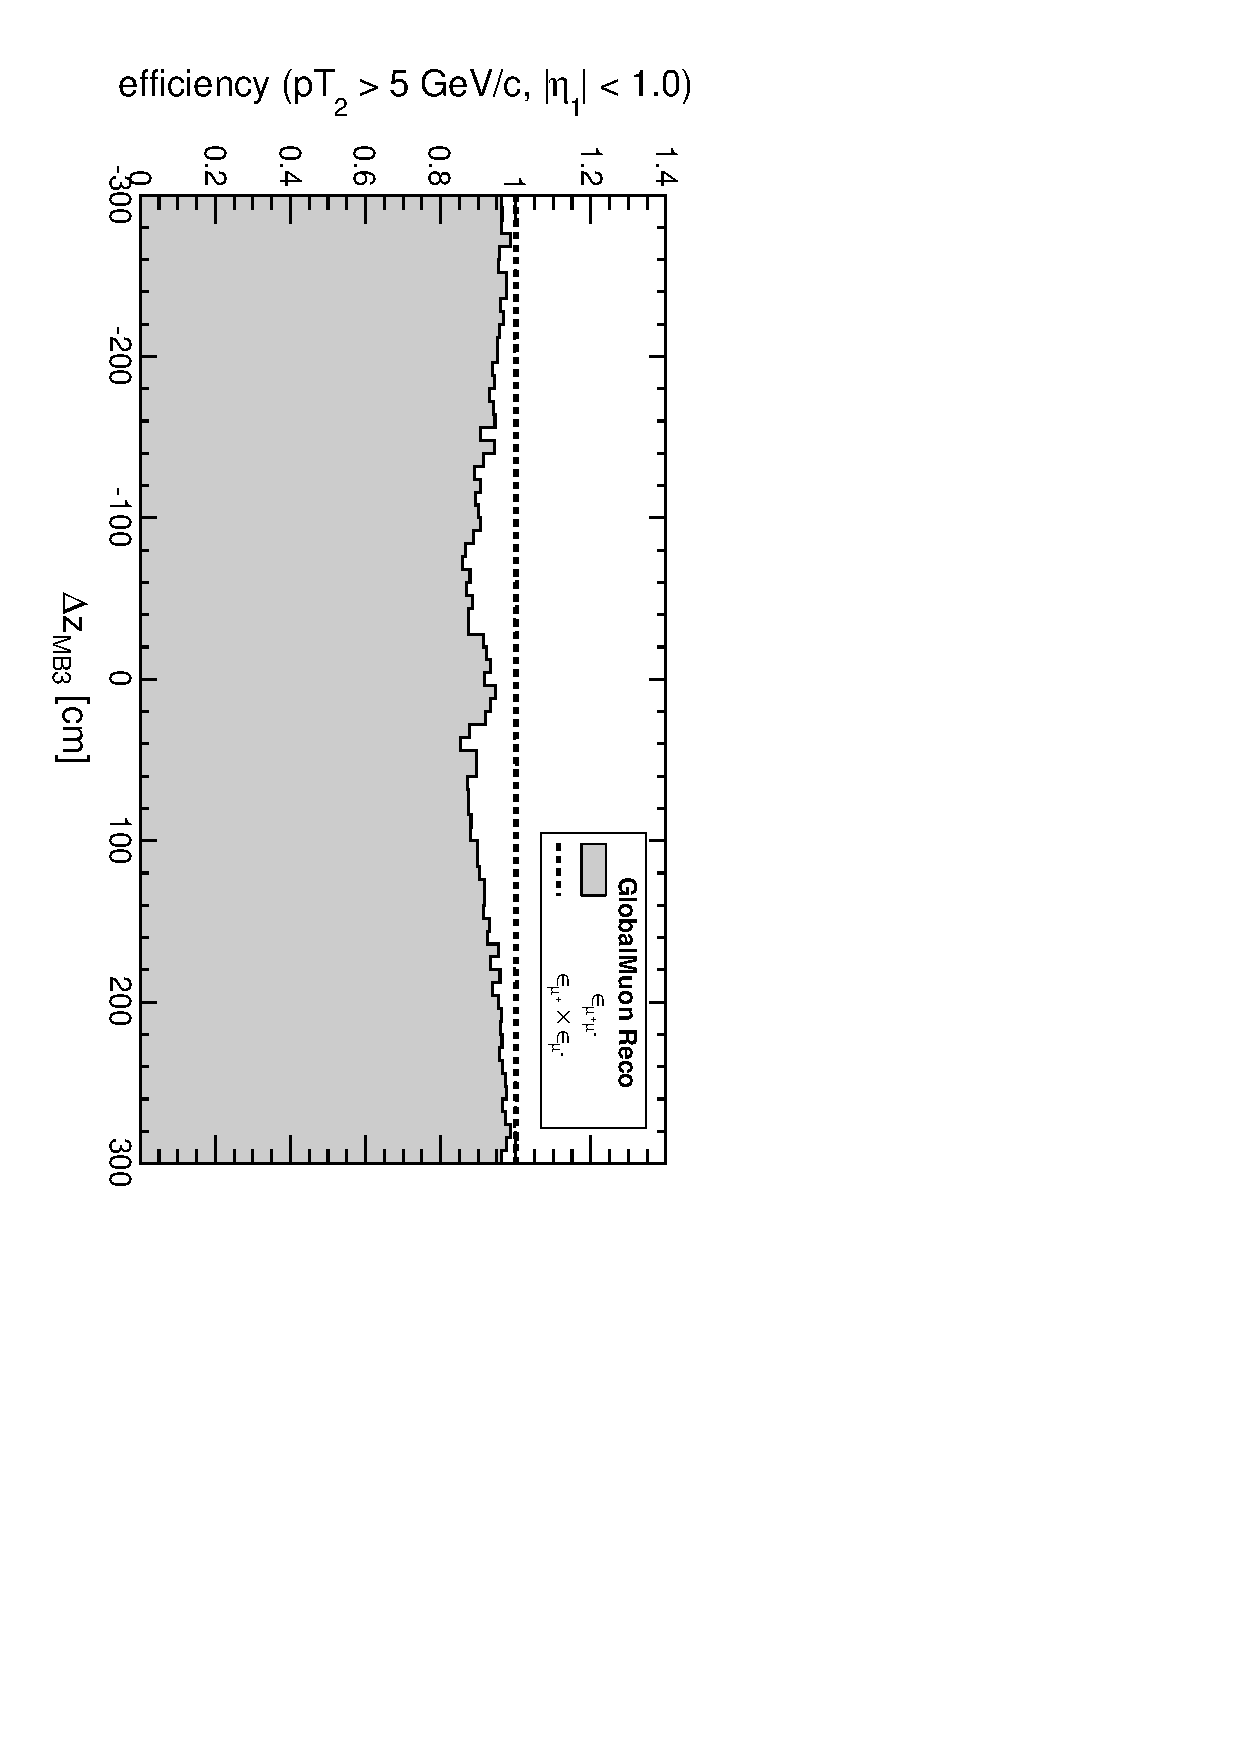
\includegraphics[height=0.45\linewidth, angle=90]{vsmb3dz_GlobalMuons.pdf}

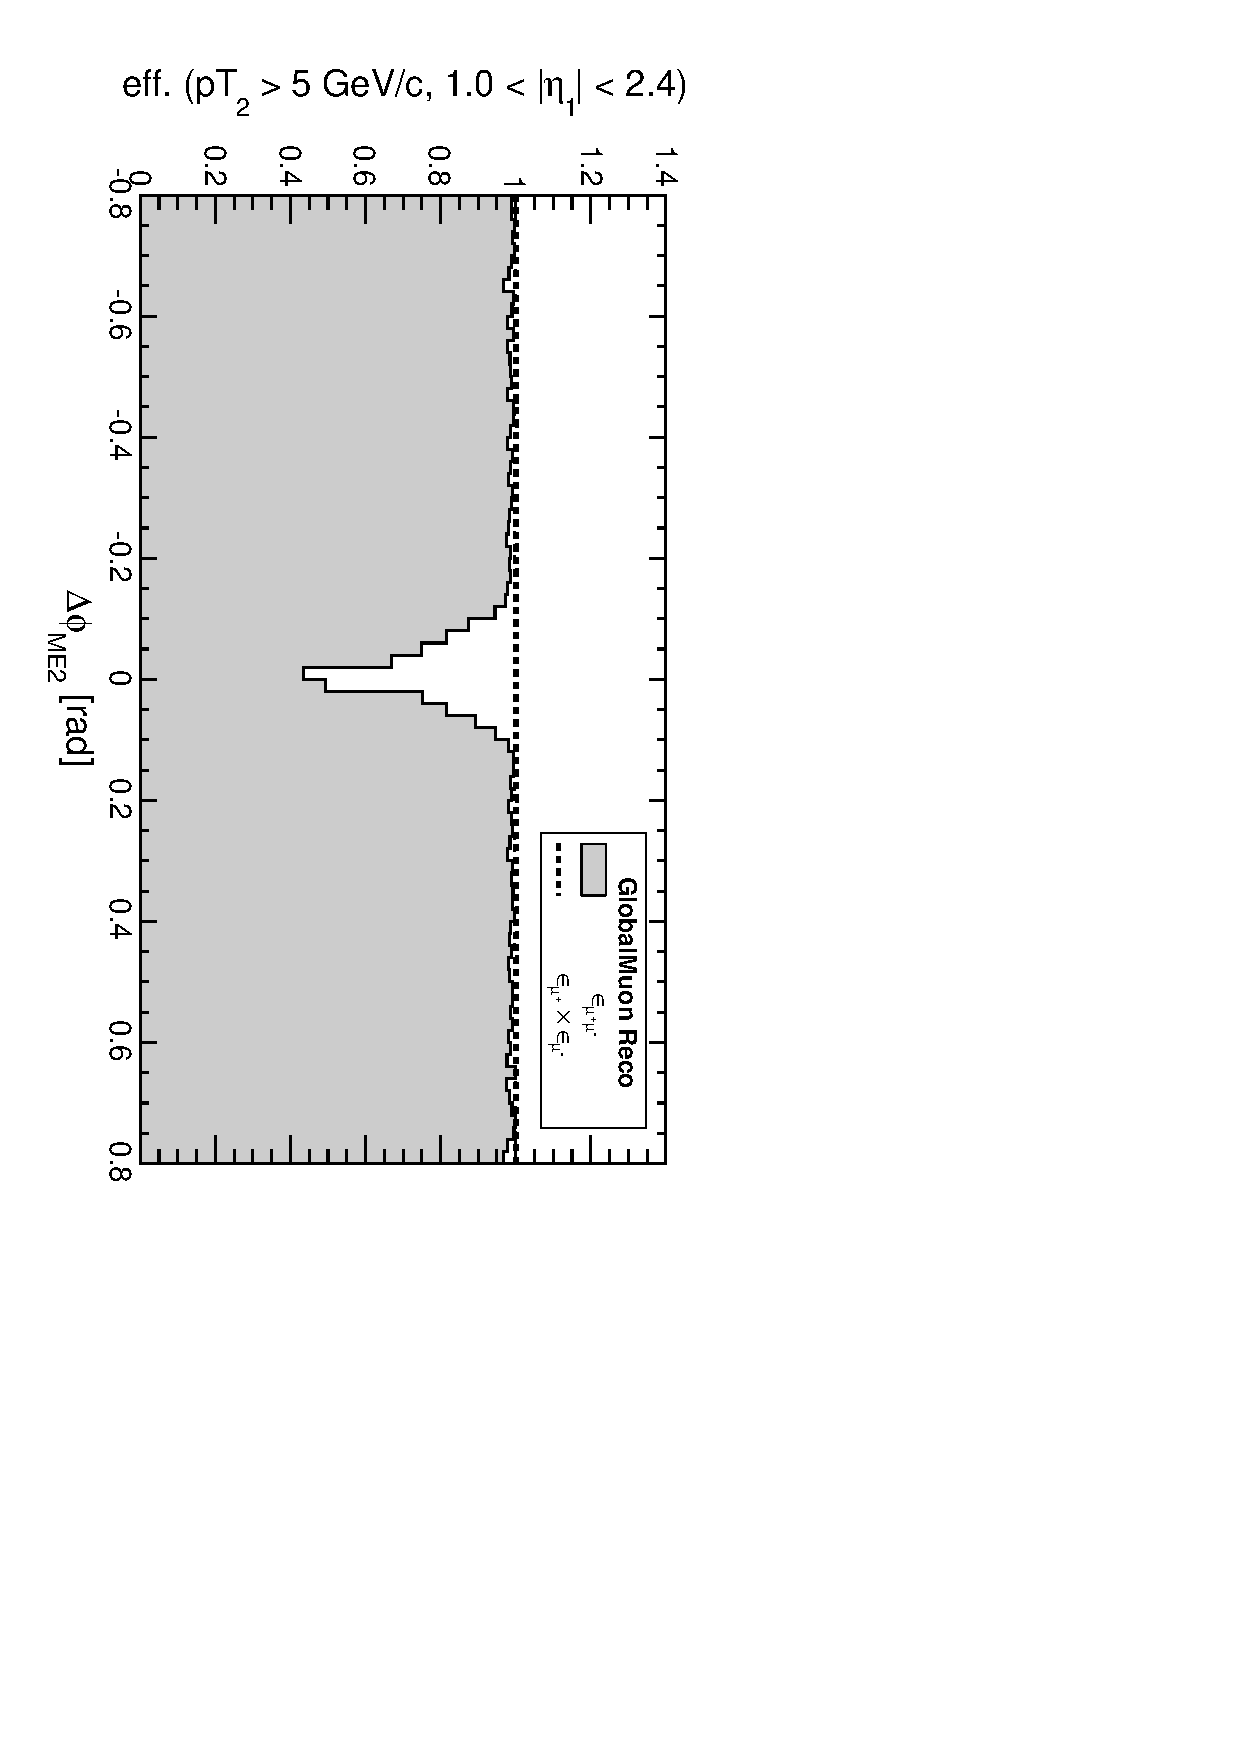
\includegraphics[height=0.45\linewidth, angle=90]{vsme2dphi_GlobalMuons.pdf}
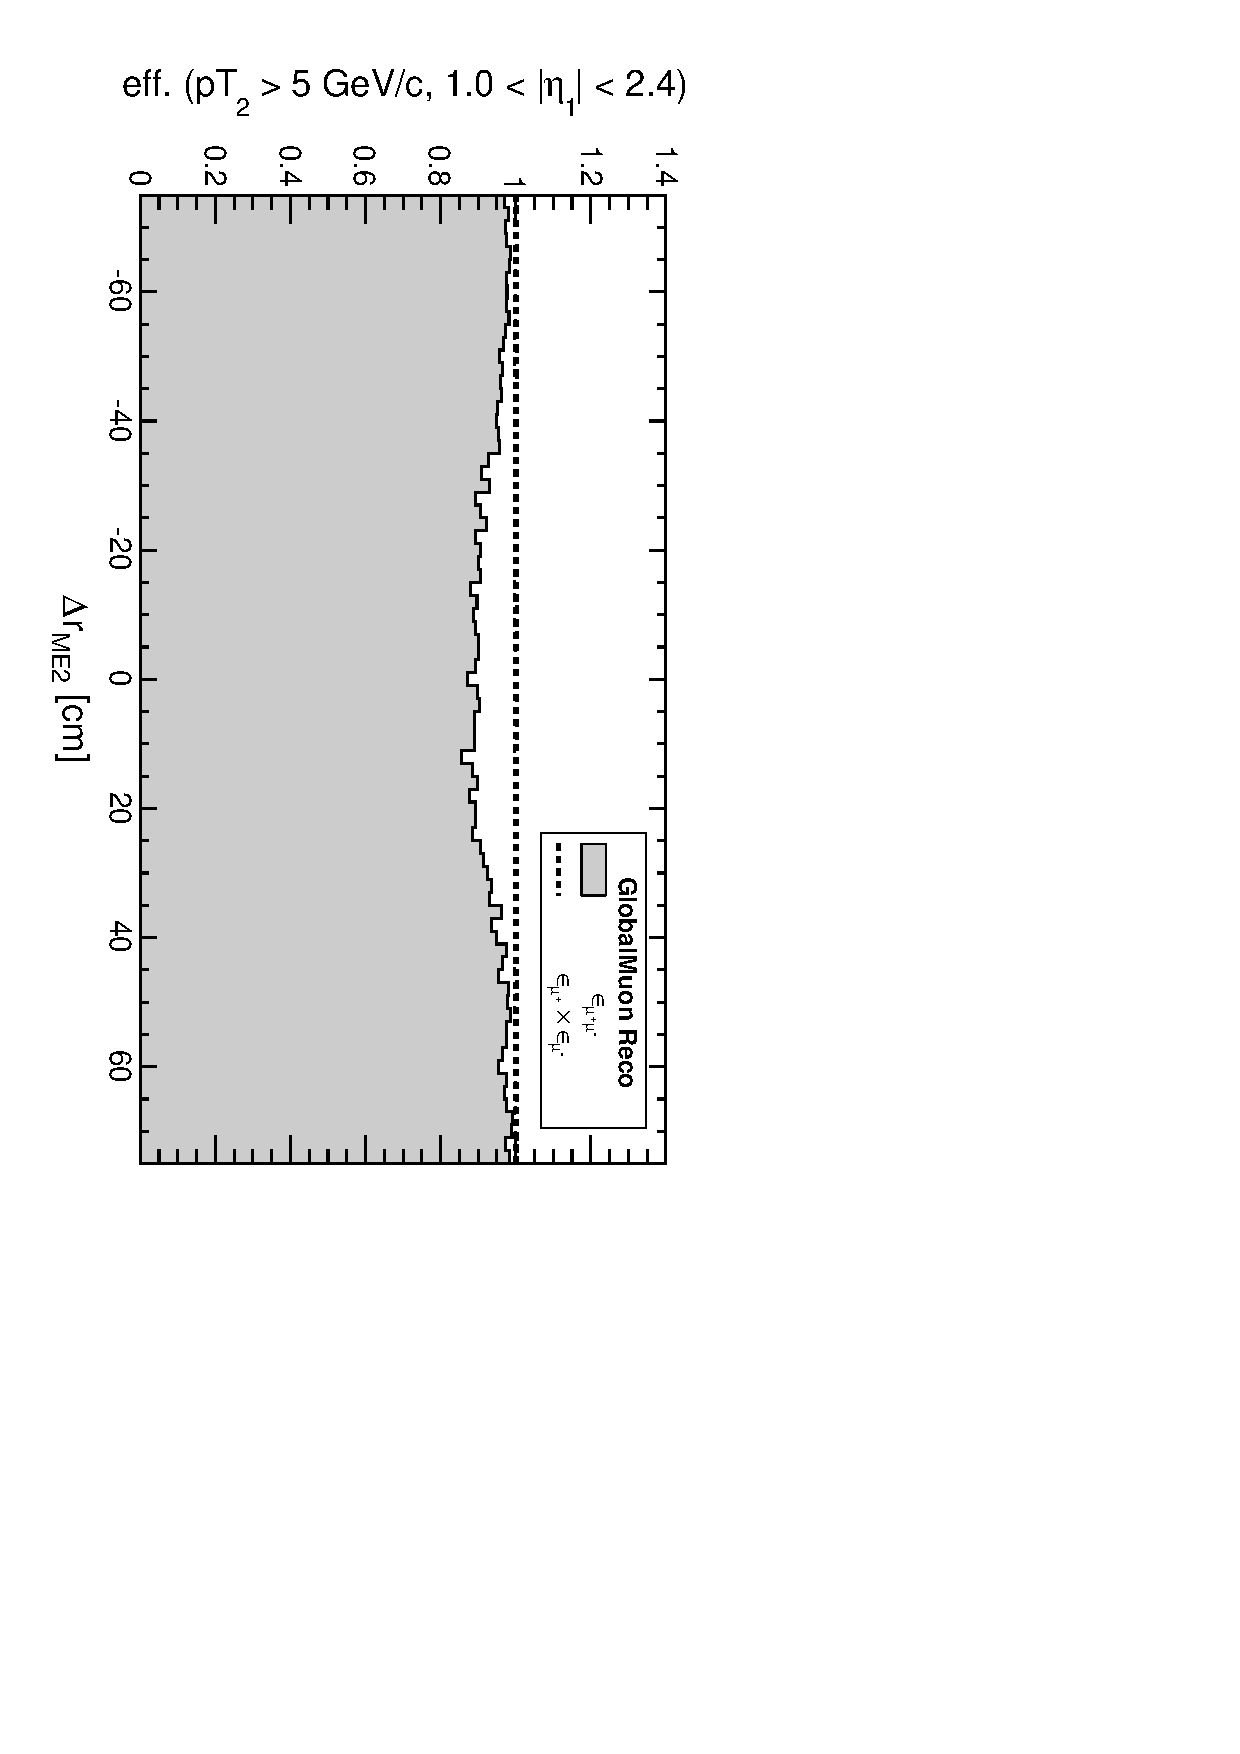
\includegraphics[height=0.45\linewidth, angle=90]{vsme2dr_GlobalMuons.pdf}
\end{frame}

\begin{frame}
\frametitle{Efficiency plots}
\framesubtitle{Same vs.\ other variables}

\begin{itemize}
\item vs.\ separation at origin
\end{itemize}

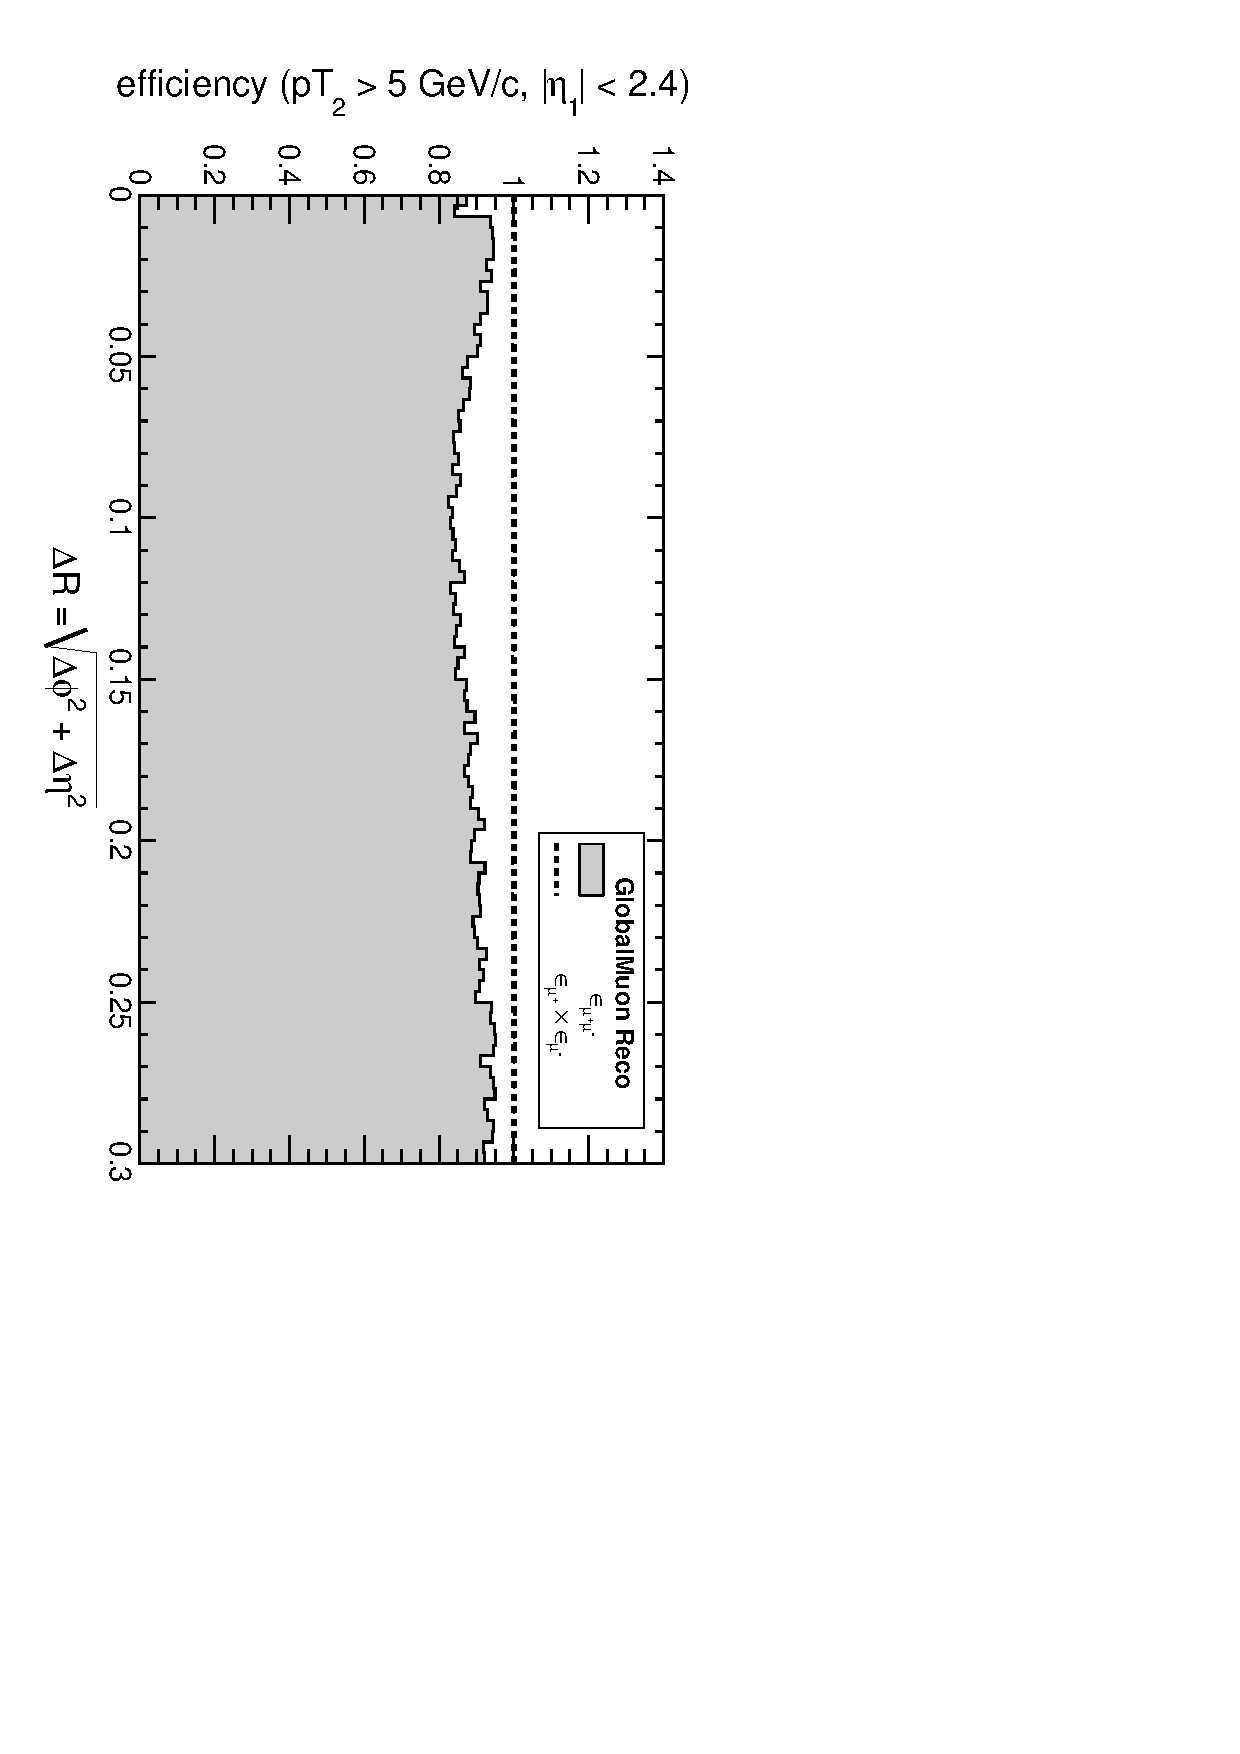
\includegraphics[height=0.5\linewidth, angle=90]{vsdR_GlobalMuons.pdf}
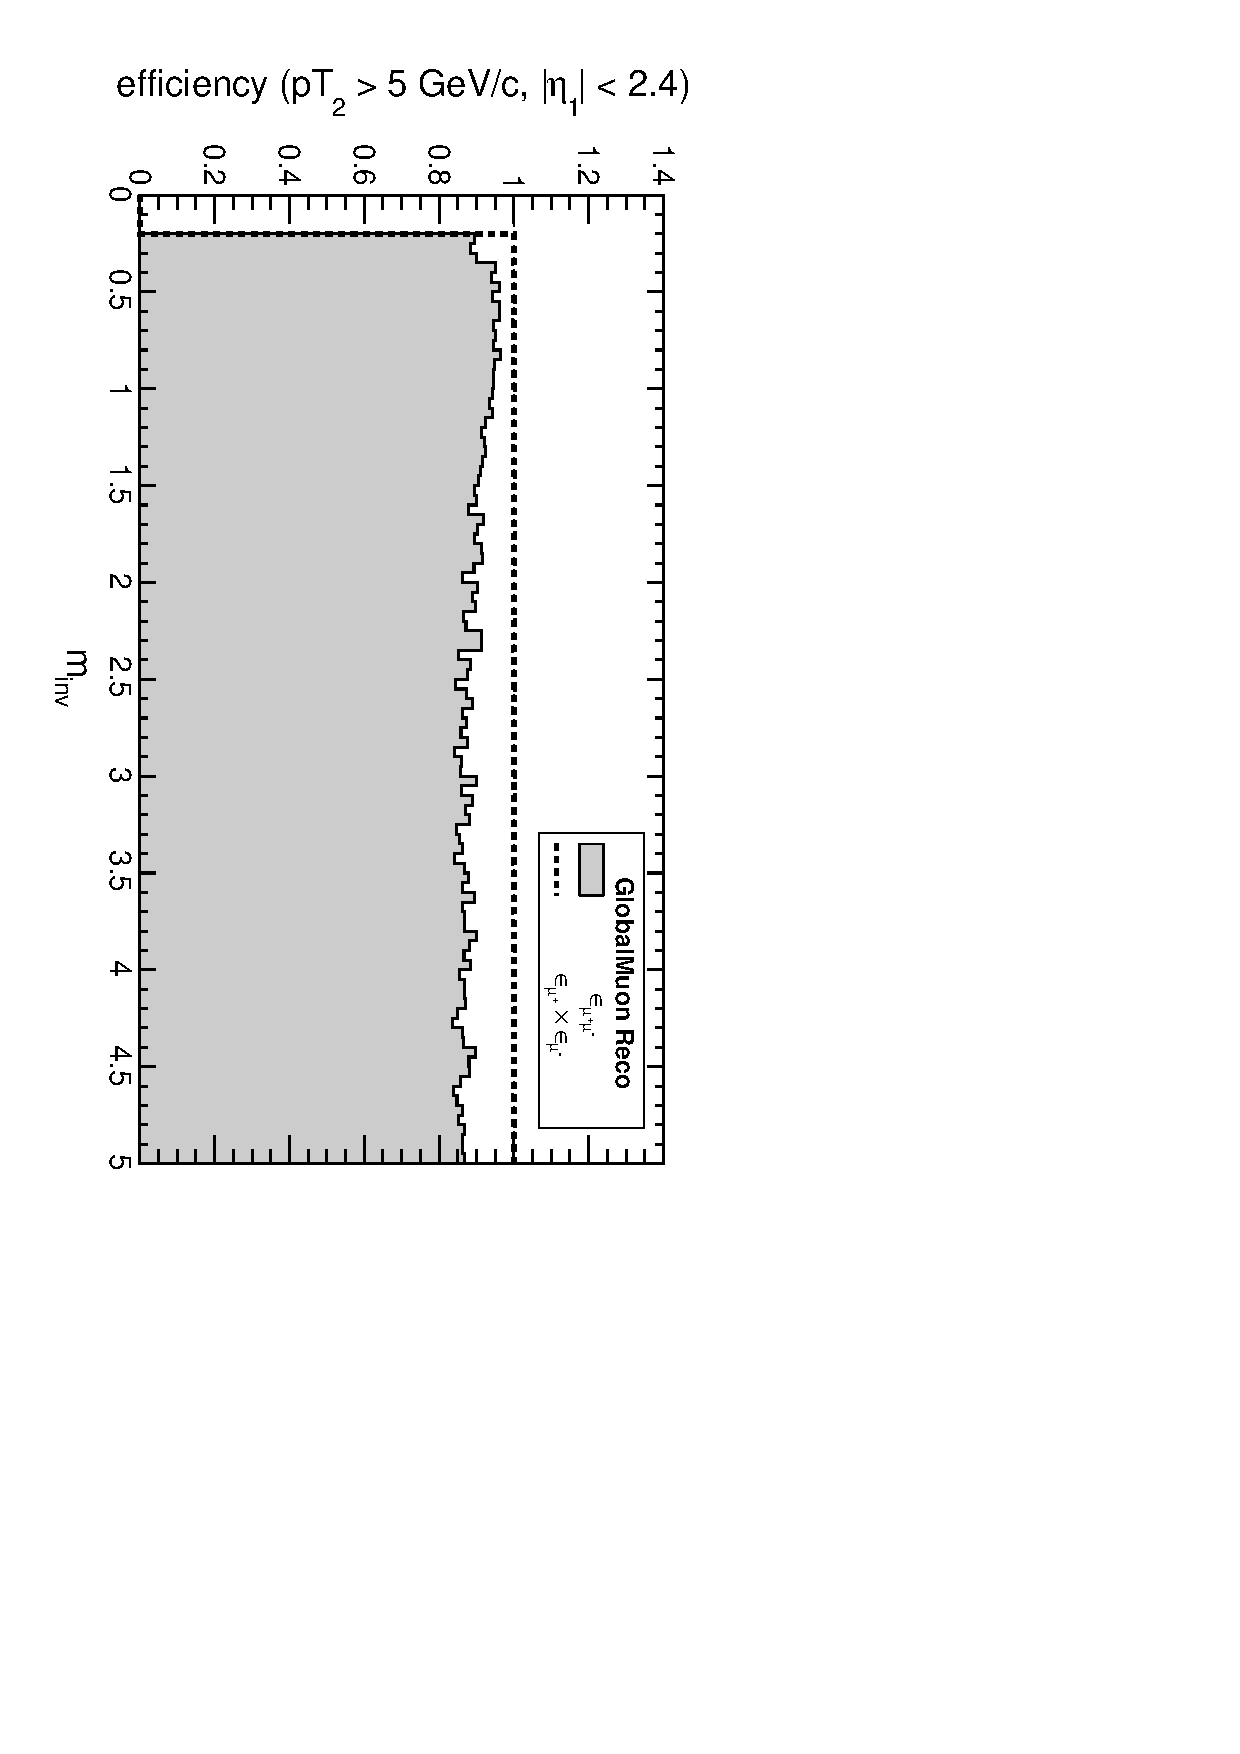
\includegraphics[height=0.5\linewidth, angle=90]{vsmass_GlobalMuons.pdf}
\end{frame}

\begin{frame}
\frametitle{Efficiency plots}
\framesubtitle{Trigger efficiency using the same technique}

\begin{itemize}
\item Can study trigger efficiencies the same way
\item Now we compare $\epsilon_{\mu^+\mu^-}$ with $1 - (1 - \epsilon_{\mu^+}) \times (1 - \epsilon_{\mu^-})$ because a single-muon trigger will fire if $\mu^+$ {\bf or} $\mu^-$ is detected
\item But I want to try some simple test-cases before I'm sure that the machinery is working
\end{itemize}

\vfill
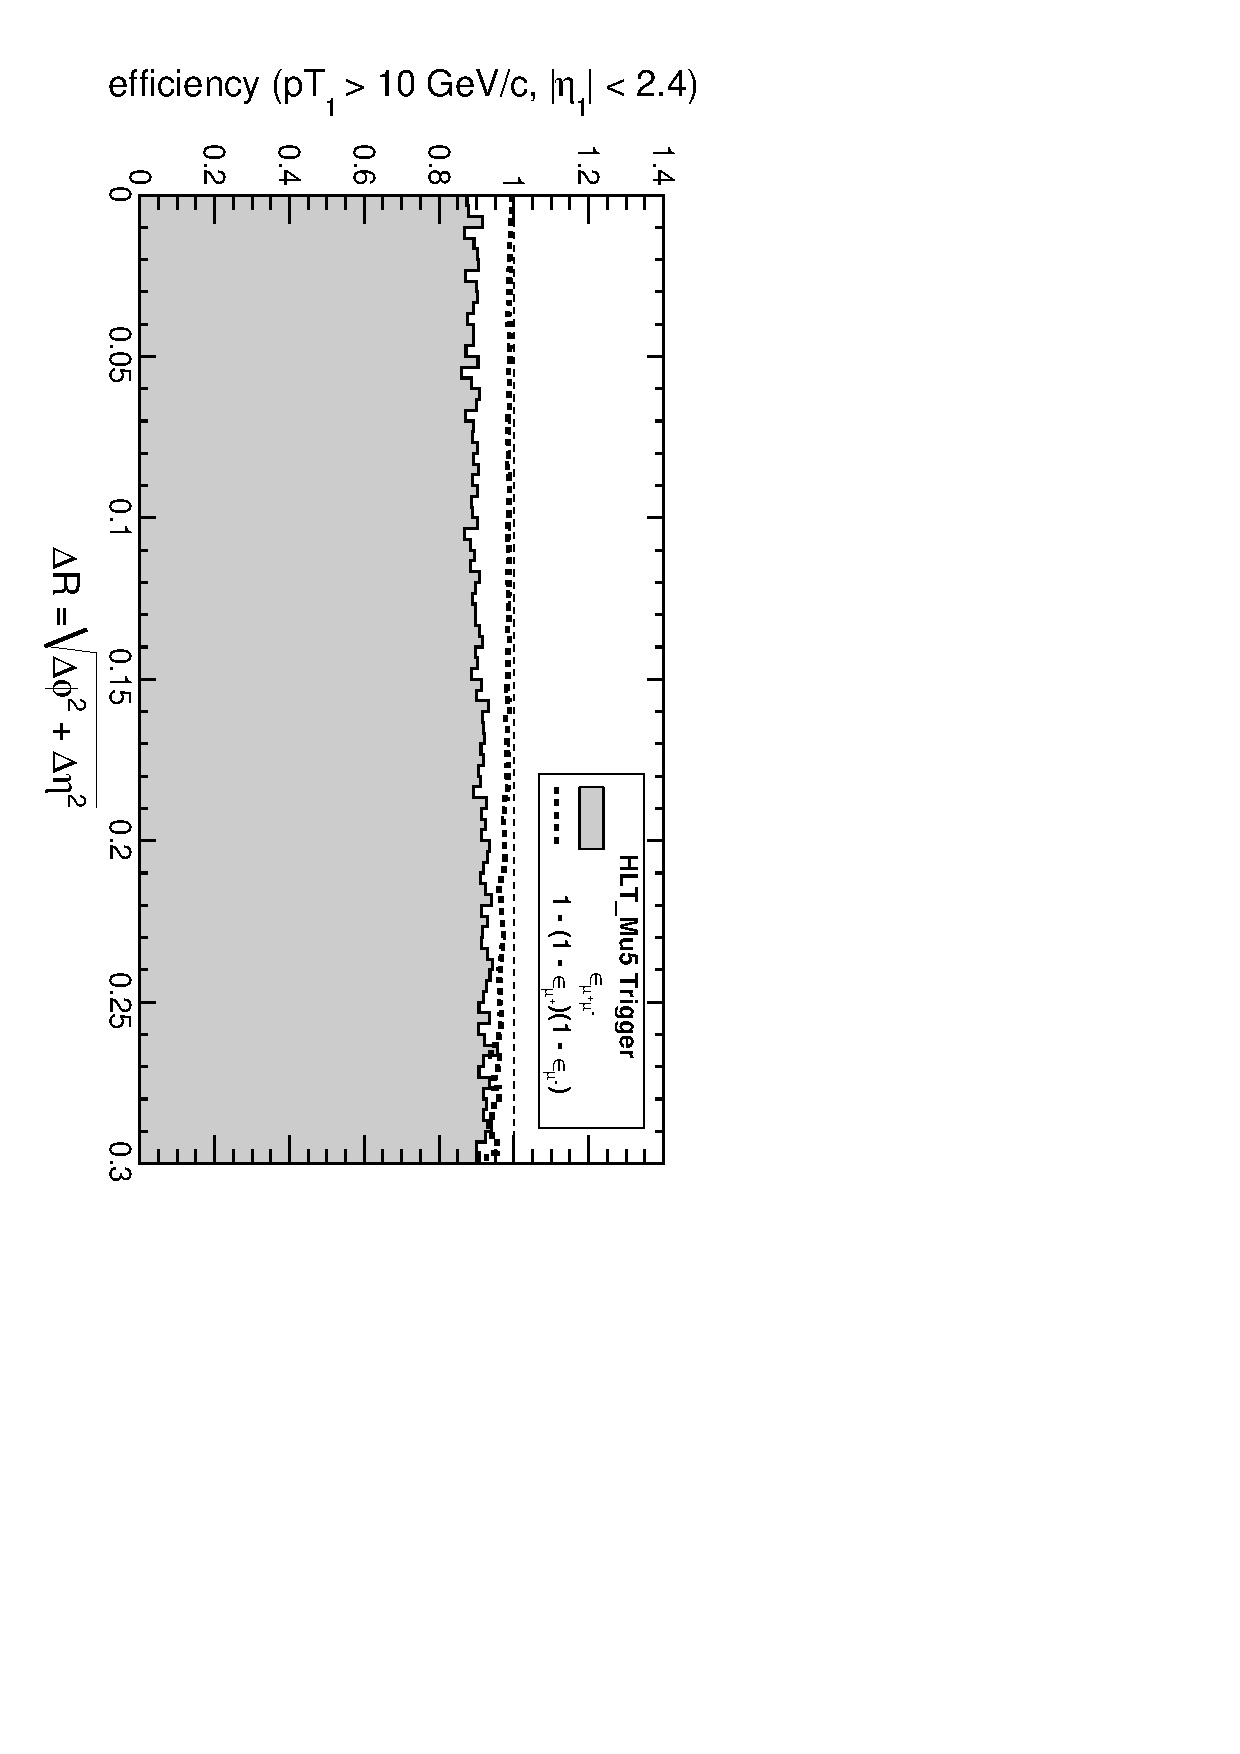
\includegraphics[height=0.3\linewidth, angle=90]{vsdR_HLT_Mu5.pdf}
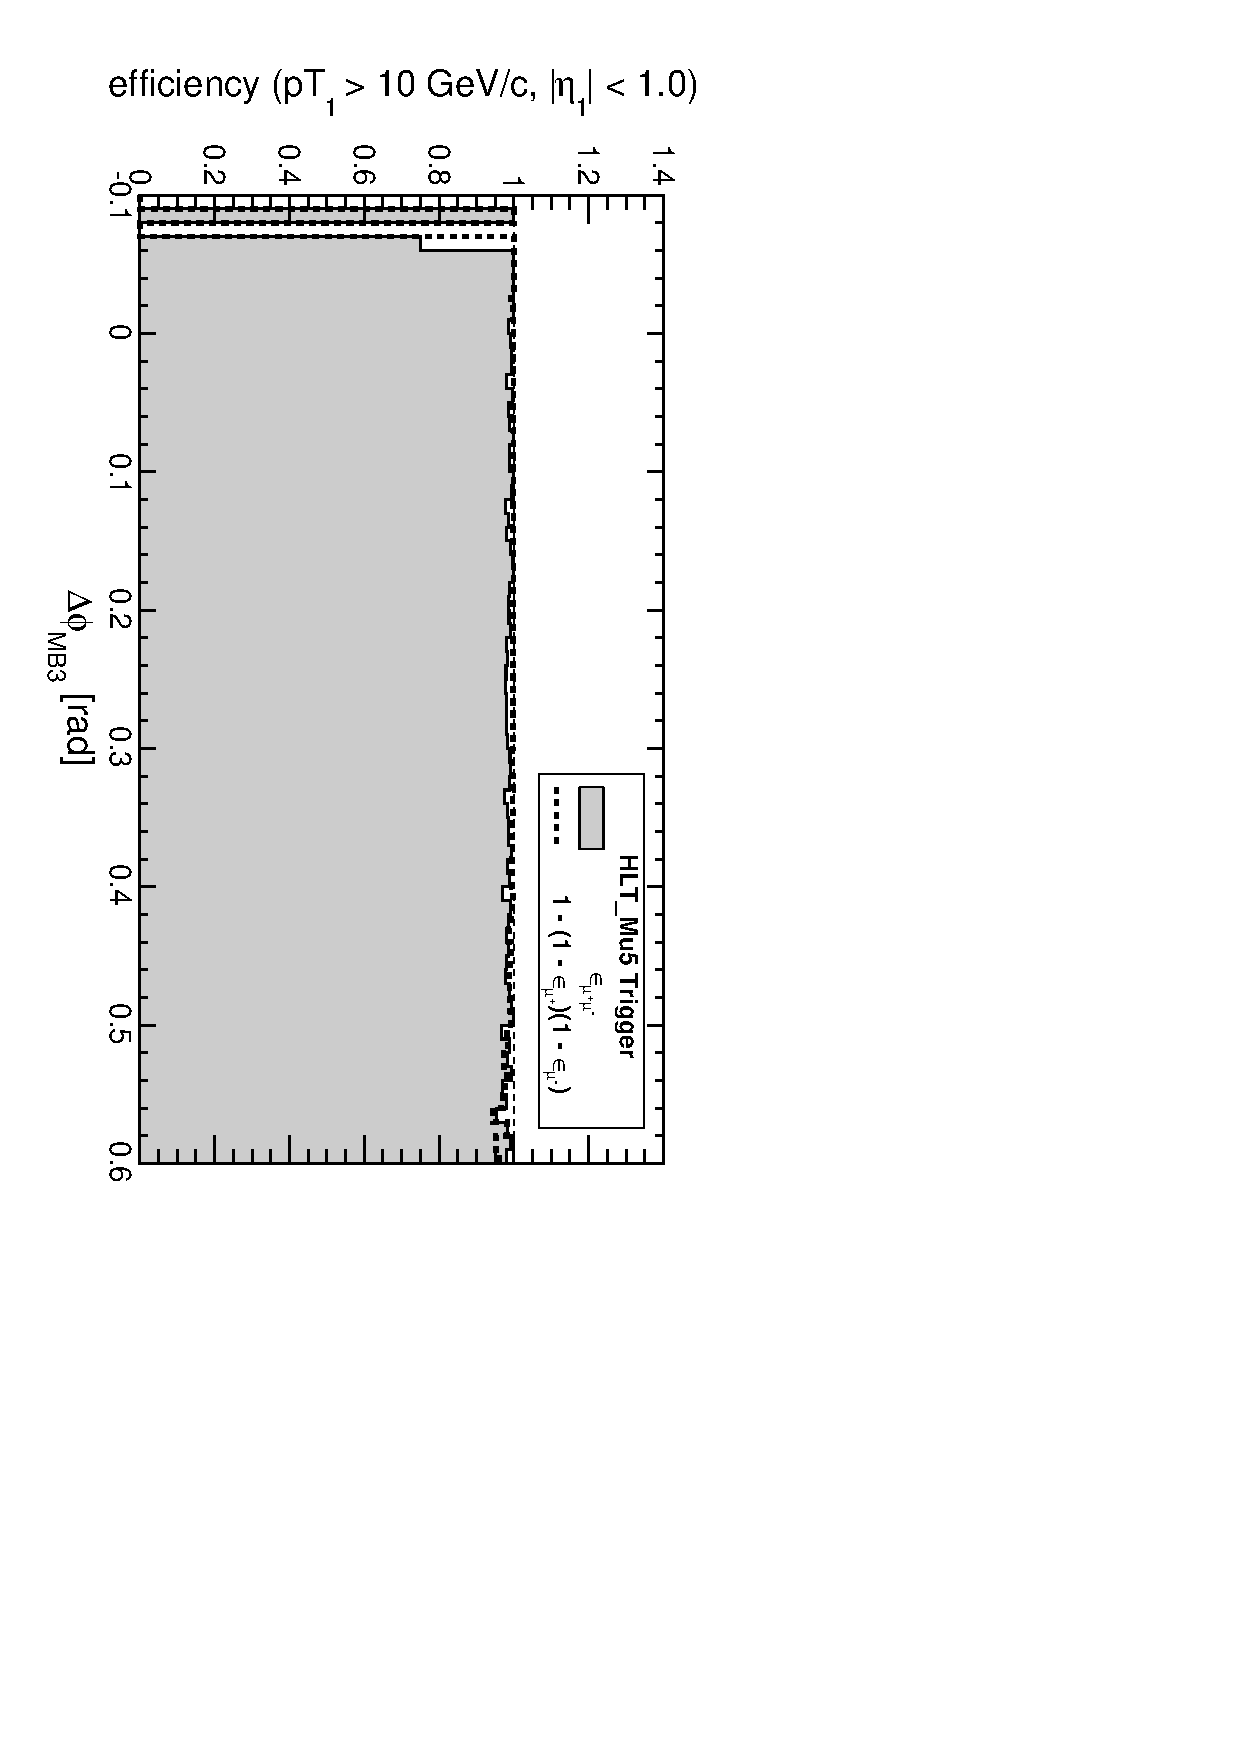
\includegraphics[height=0.3\linewidth, angle=90]{vsmb3dphi_HLT_Mu5.pdf}
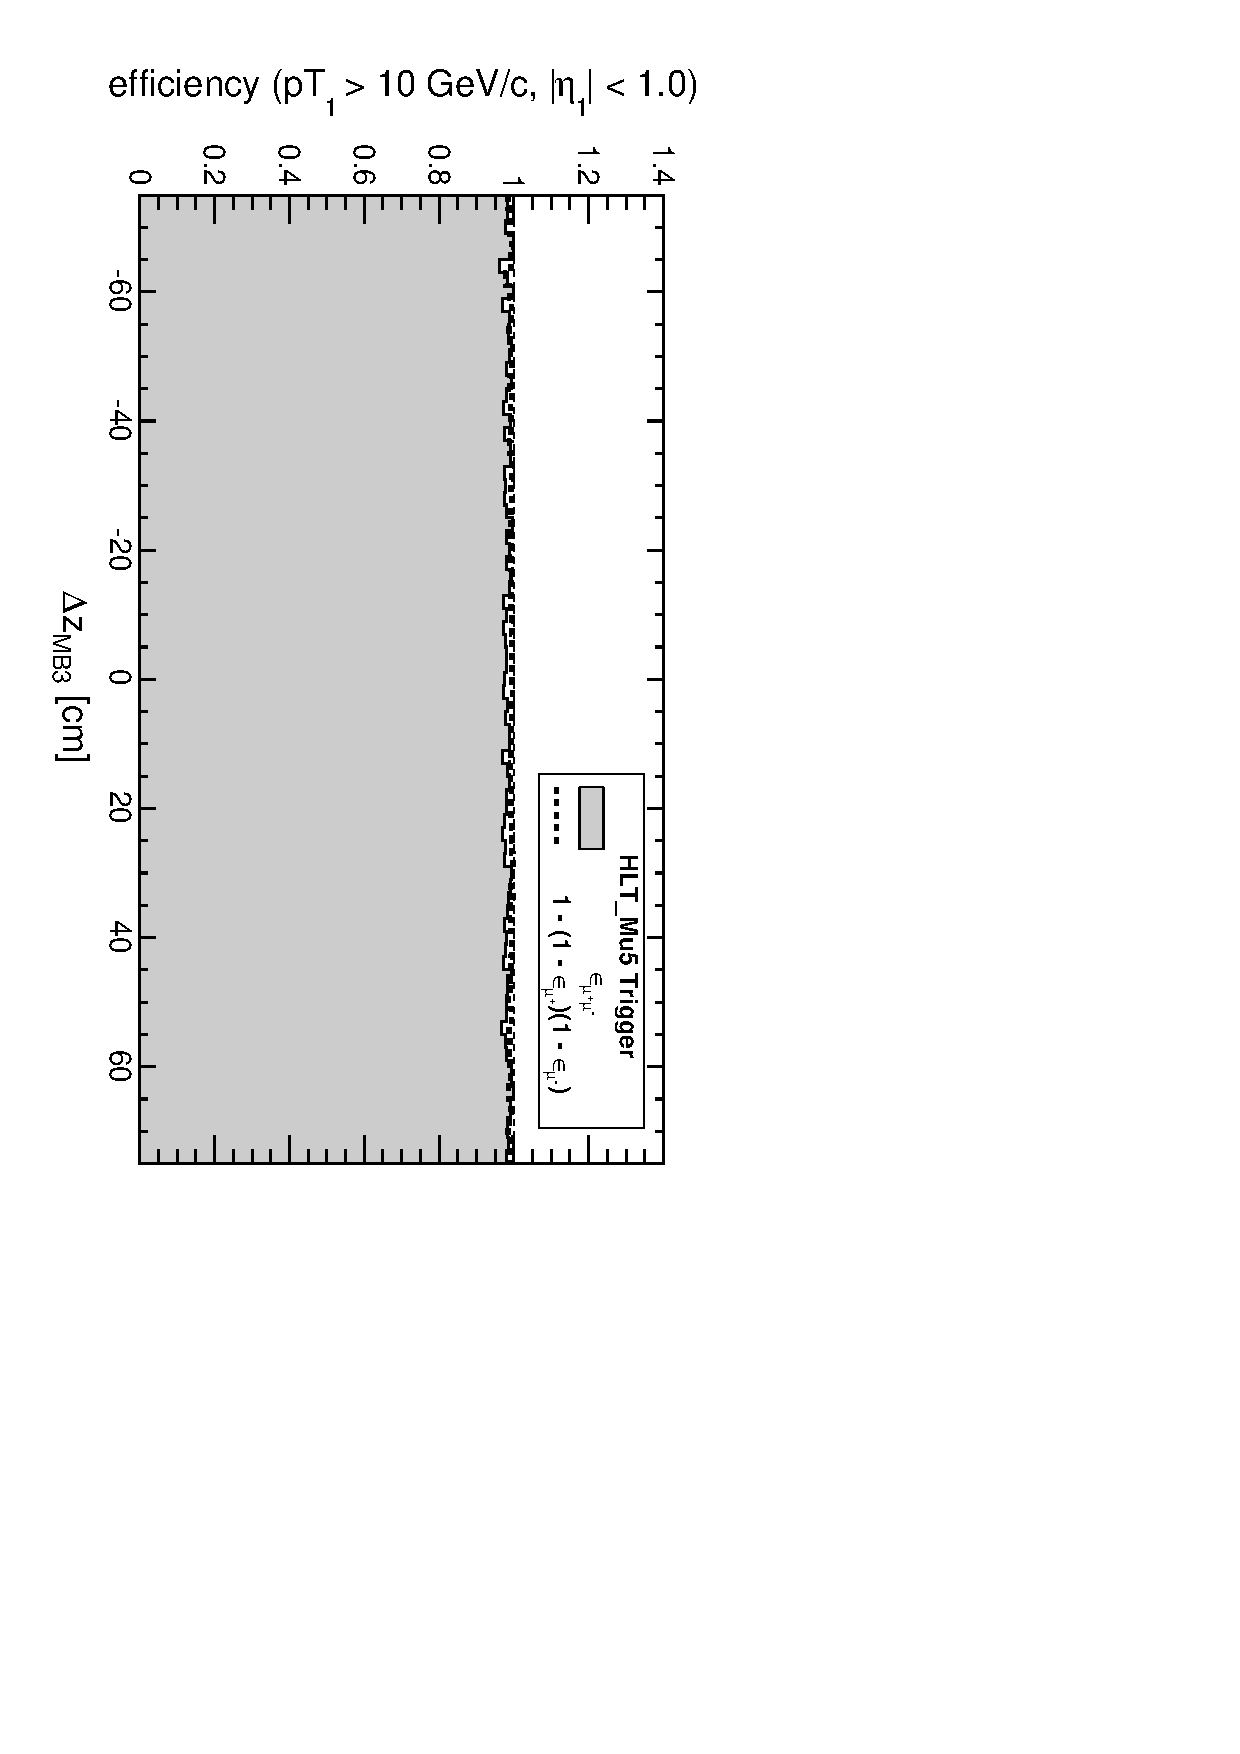
\includegraphics[height=0.3\linewidth, angle=90]{vsmb3dz_HLT_Mu5.pdf}

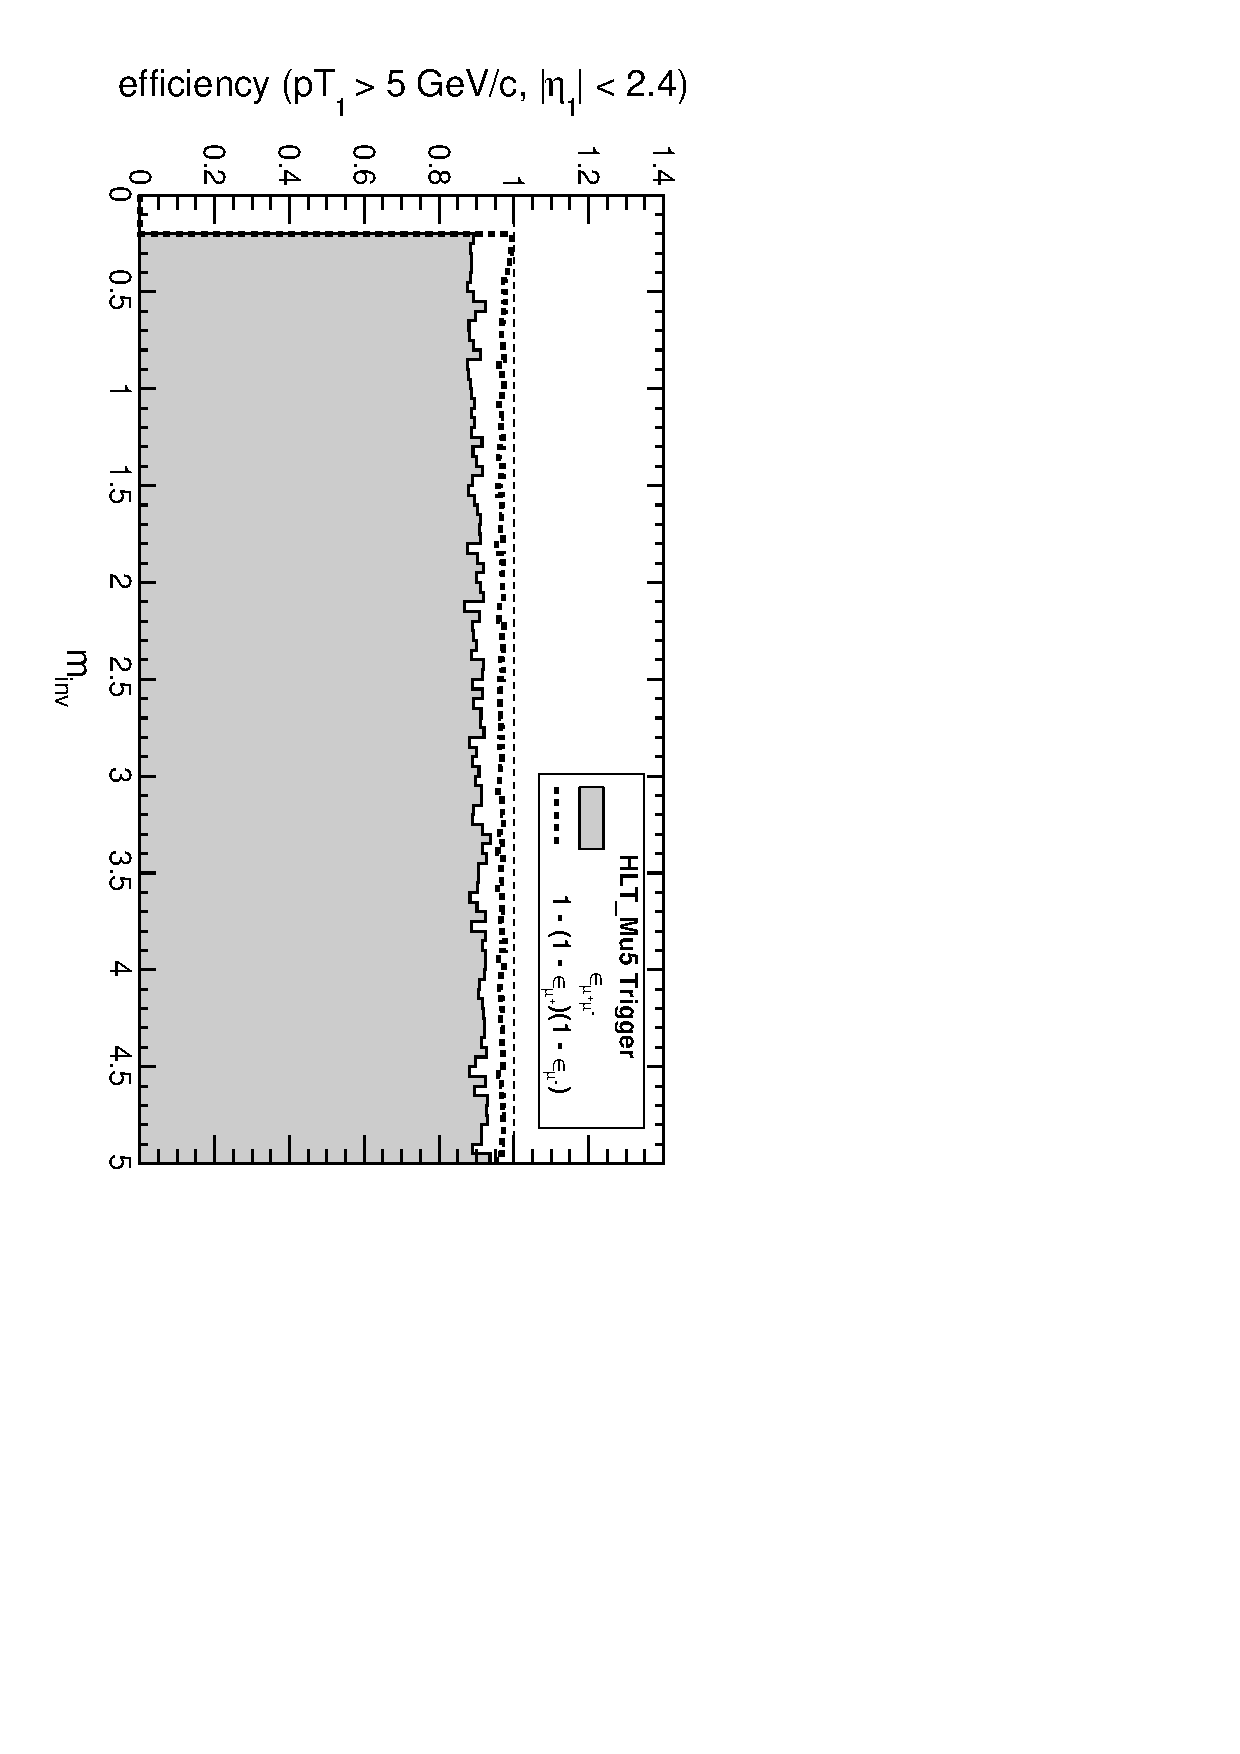
\includegraphics[height=0.3\linewidth, angle=90]{vsmass_HLT_Mu5.pdf}
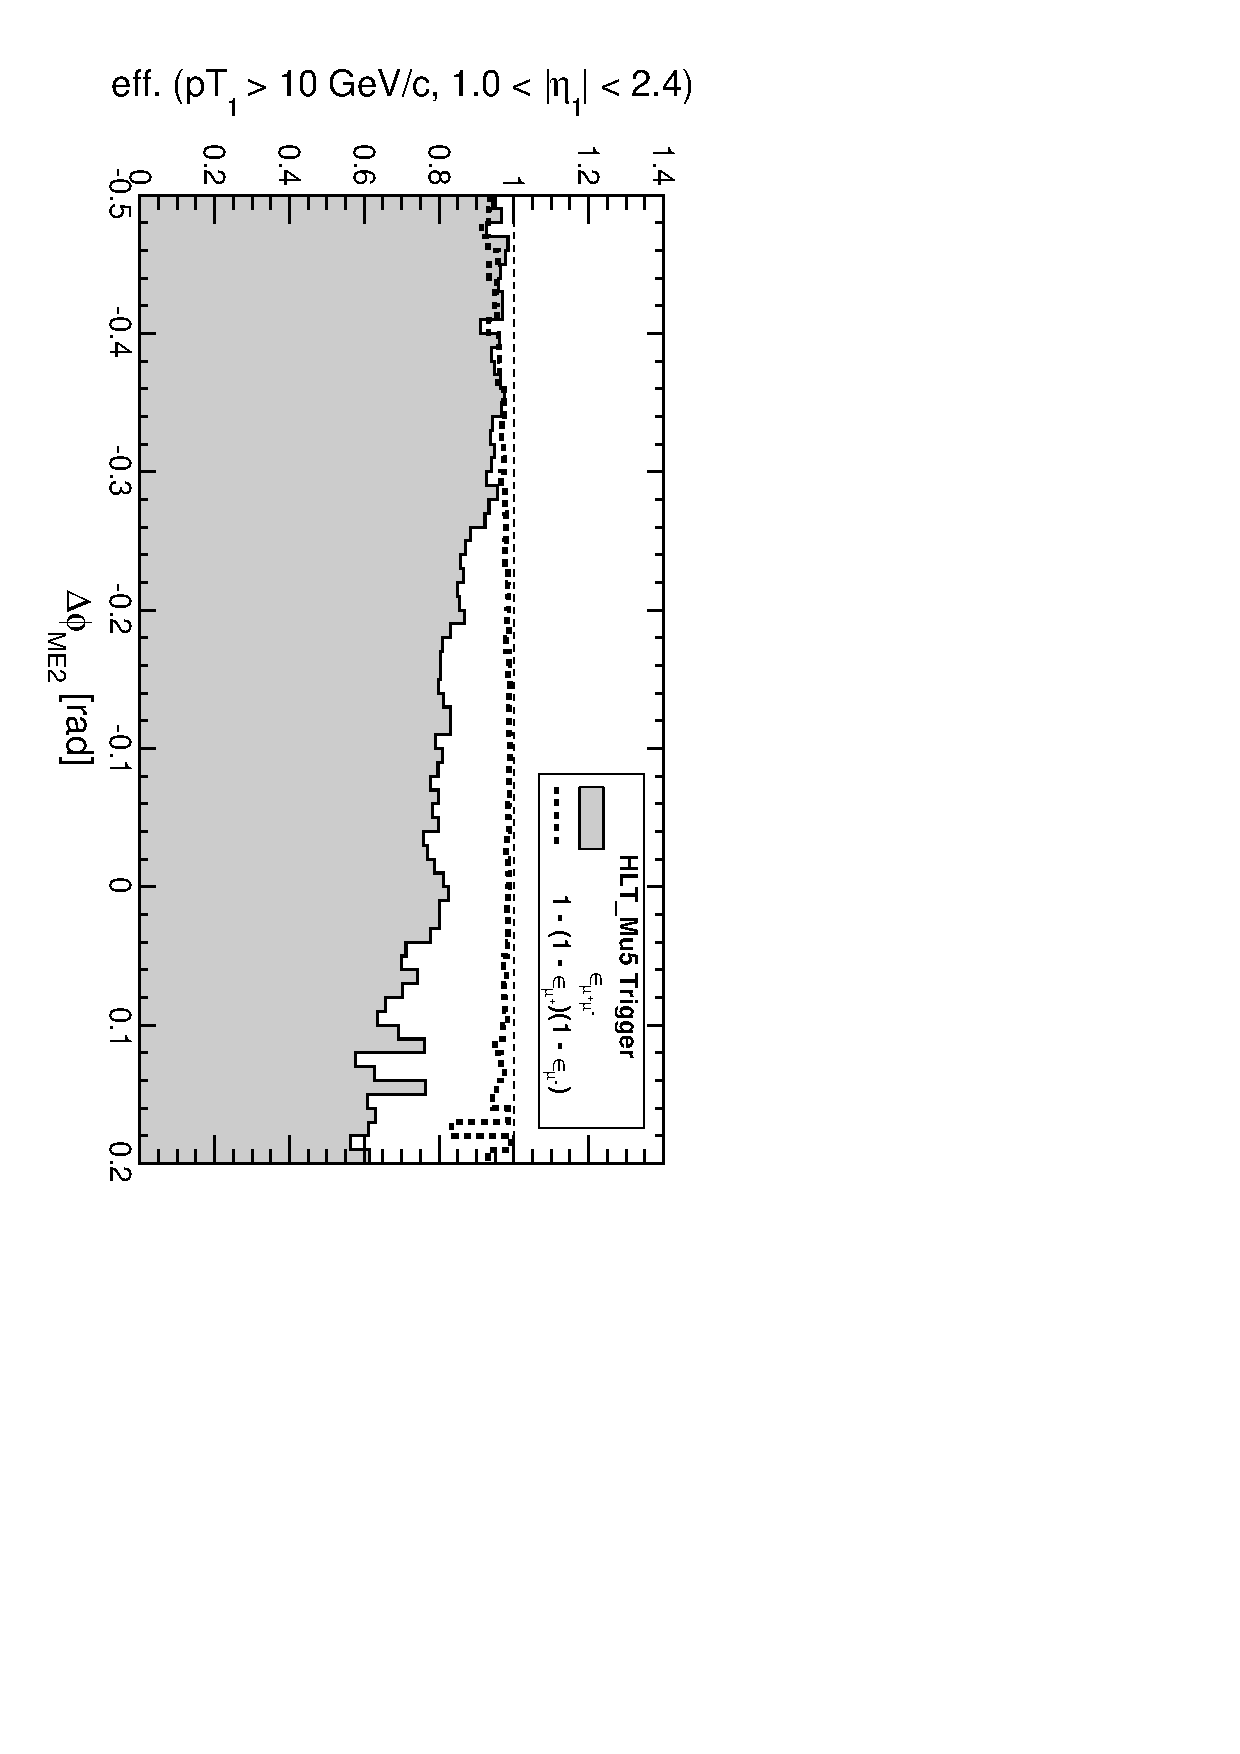
\includegraphics[height=0.3\linewidth, angle=90]{vsme2dphi_HLT_Mu5.pdf}
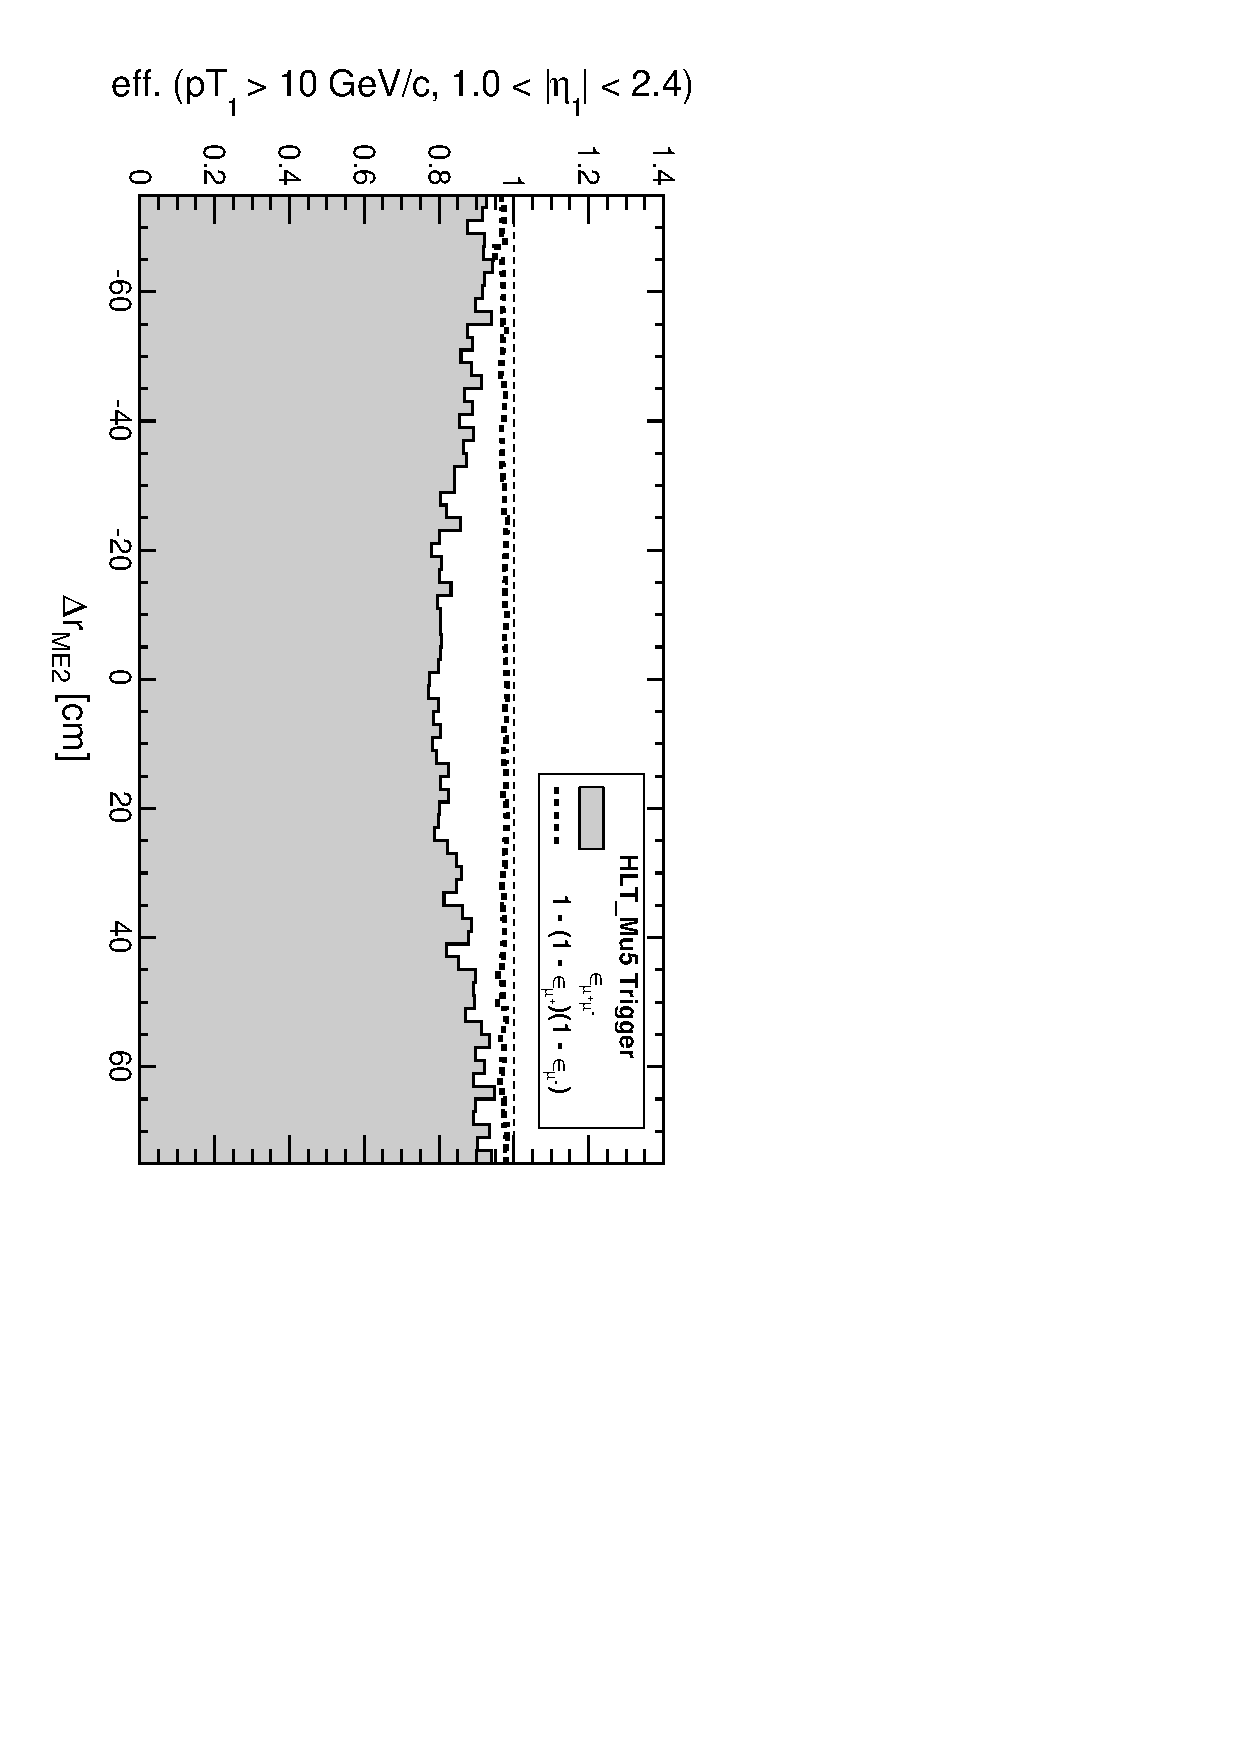
\includegraphics[height=0.3\linewidth, angle=90]{vsme2dr_HLT_Mu5.pdf}
\end{frame}

\begin{frame}
\frametitle{On to backgrounds}
\framesubtitle{First, a technical note}

\begin{itemize}
\item InclusiveMu5\_Pt* was produced in 5 bins of $\hat{p}_T$: 30+, 50+, 150+, 250+, and 350+ GeV/$c$
\item Need to combine the samples, cut out double-counting, and scale them all to integrated luminosity
\item On all plots, vertical axis is ``picobarns per bin'': number of events you would get if you had 1~pb of data
\item Merged of $\hat{p}_T$: no discontinuities means that merging machinery is working\ldots\ time to go on to physics plots
\end{itemize}

\vfill
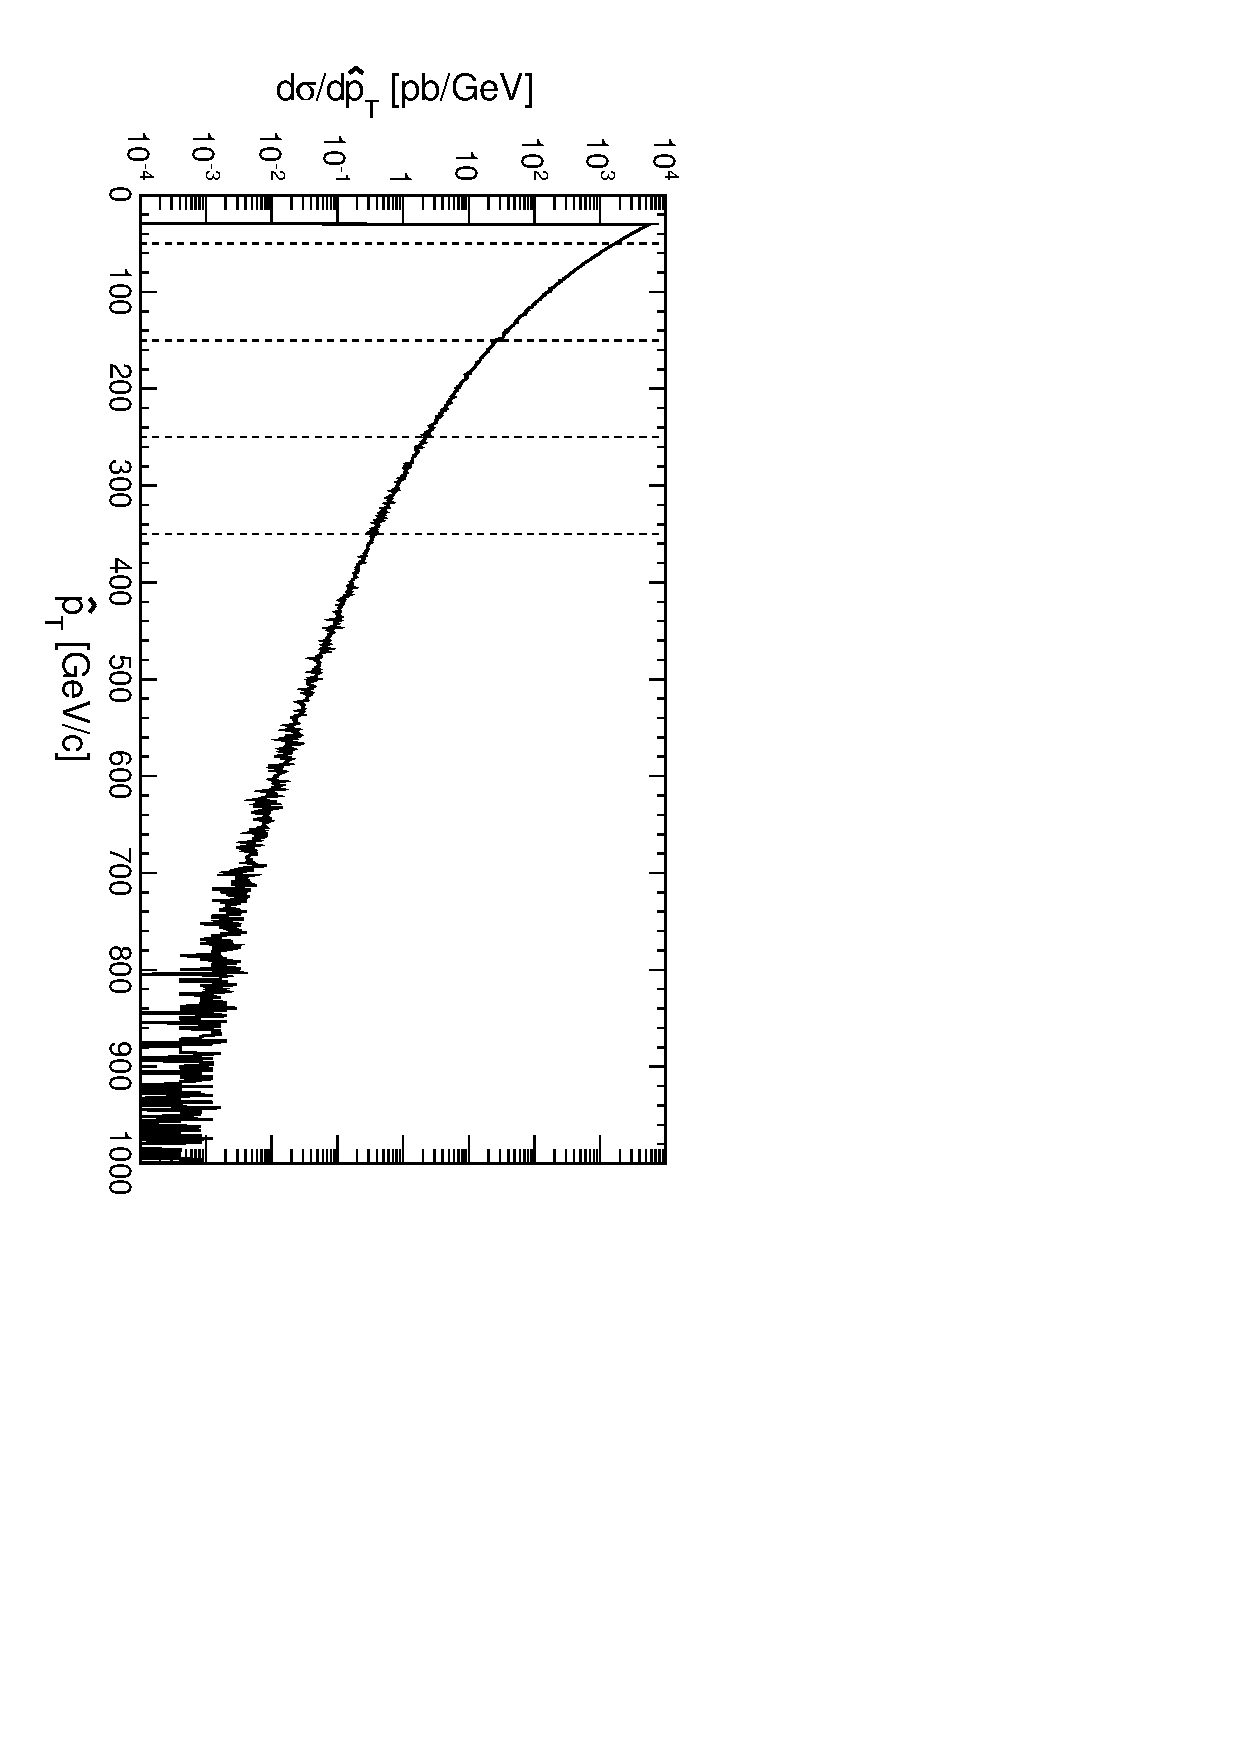
\includegraphics[height=0.5\linewidth, angle=90]{qscale.pdf}
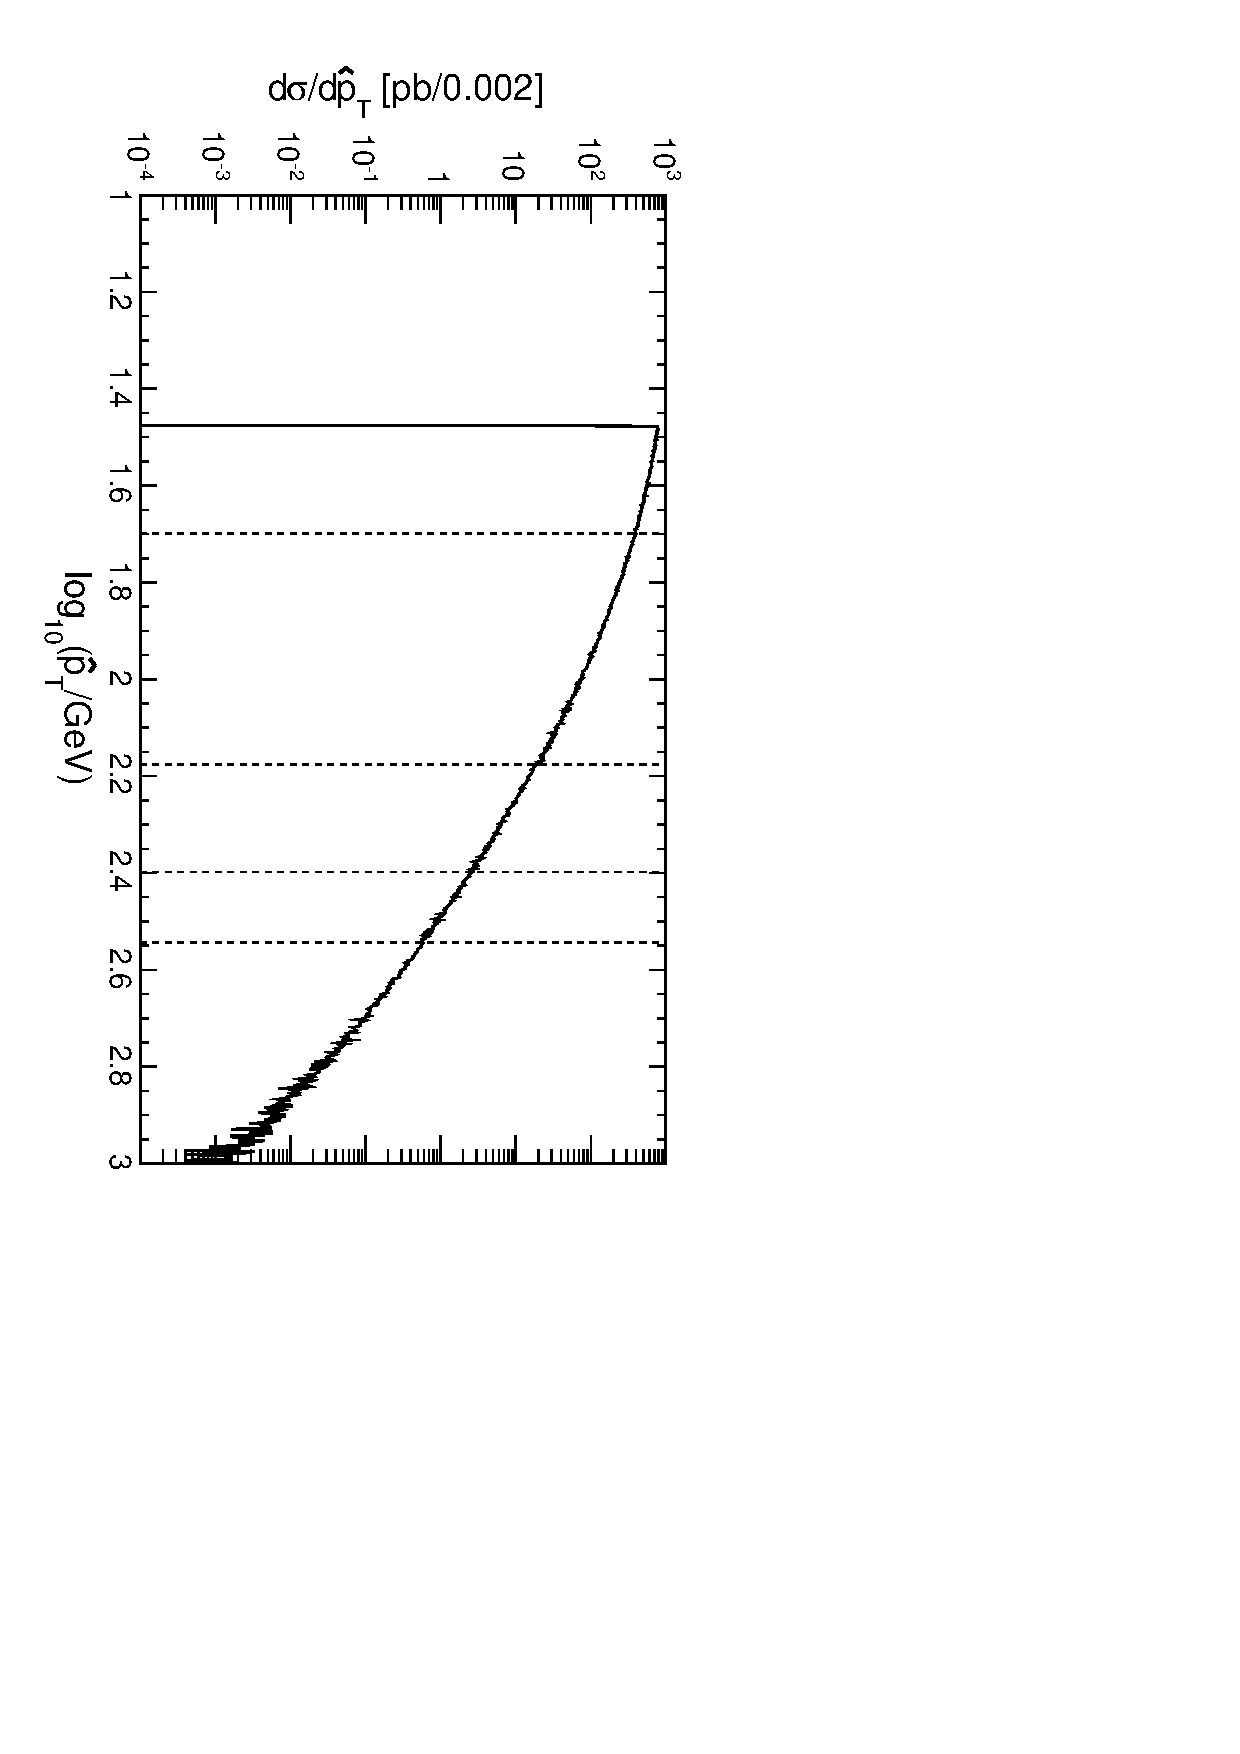
\includegraphics[height=0.5\linewidth, angle=90]{log10qscale.pdf}
\end{frame}

\begin{frame}
\frametitle{Number of real muons}

\begin{itemize}
\item Number of real muons per background event is useful, but a
  little hard to define in this sample because it contains some muons
  with $p \lesssim 1$~GeV/$c$ and $v_{xy} \gg 1$~cm
\item I tried two methods (in addition to $p_T > 5$~GeV/$c$)
\begin{enumerate}
\item look at MC-matches to all reconstructed muons (full collection: TrackerMuons, GlobalMuons, StandAloneMuons), and count the number of {\it unique} matched MC muons.  Since muon reco efficiency is high within the acceptance region, this is the set of all reconstruct{\it able} muons
\item look at the list of generator-level particles, and identify the muons which did not come from a $\pi^\pm$, $K^\pm$, or $K_L$ decay
\end{enumerate}
\end{itemize}

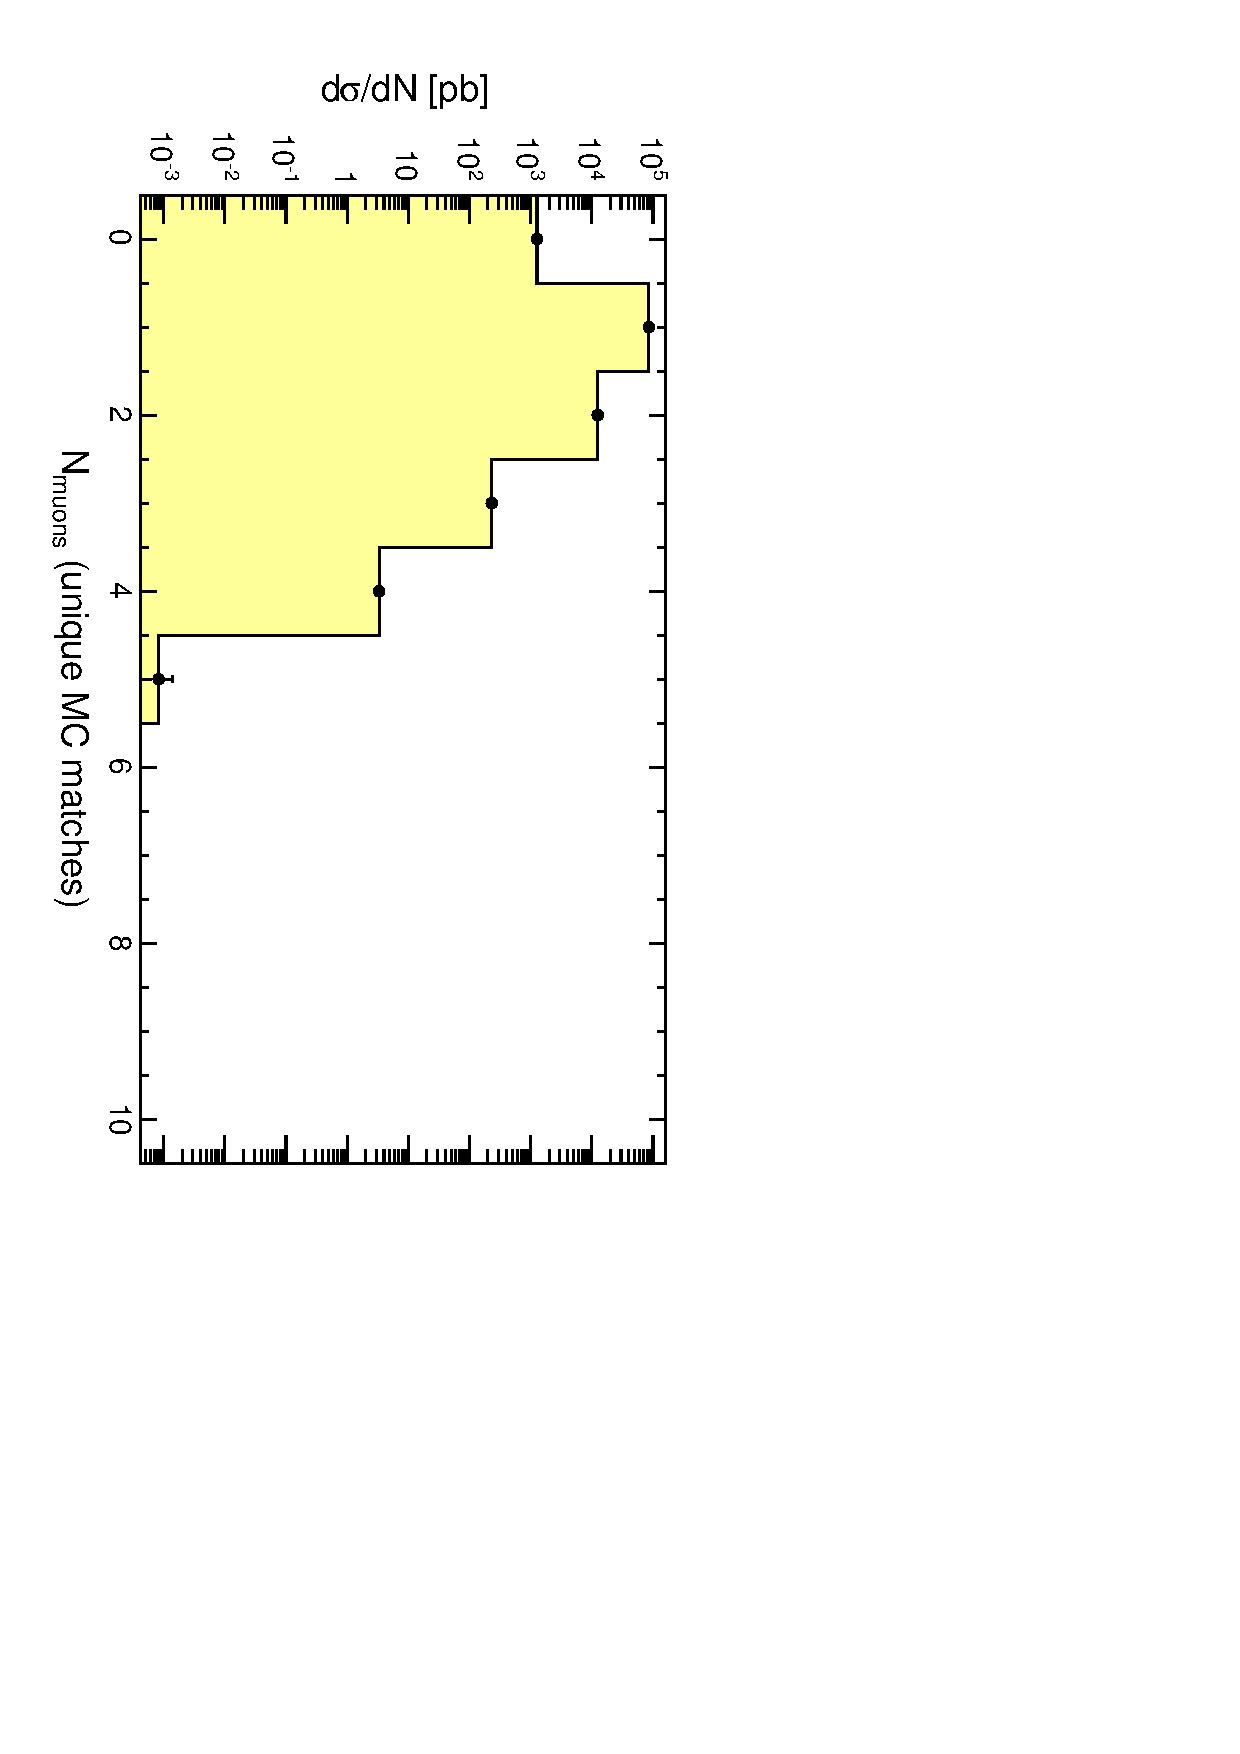
\includegraphics[height=0.5\linewidth, angle=90]{nmuons_real_Matching.pdf}
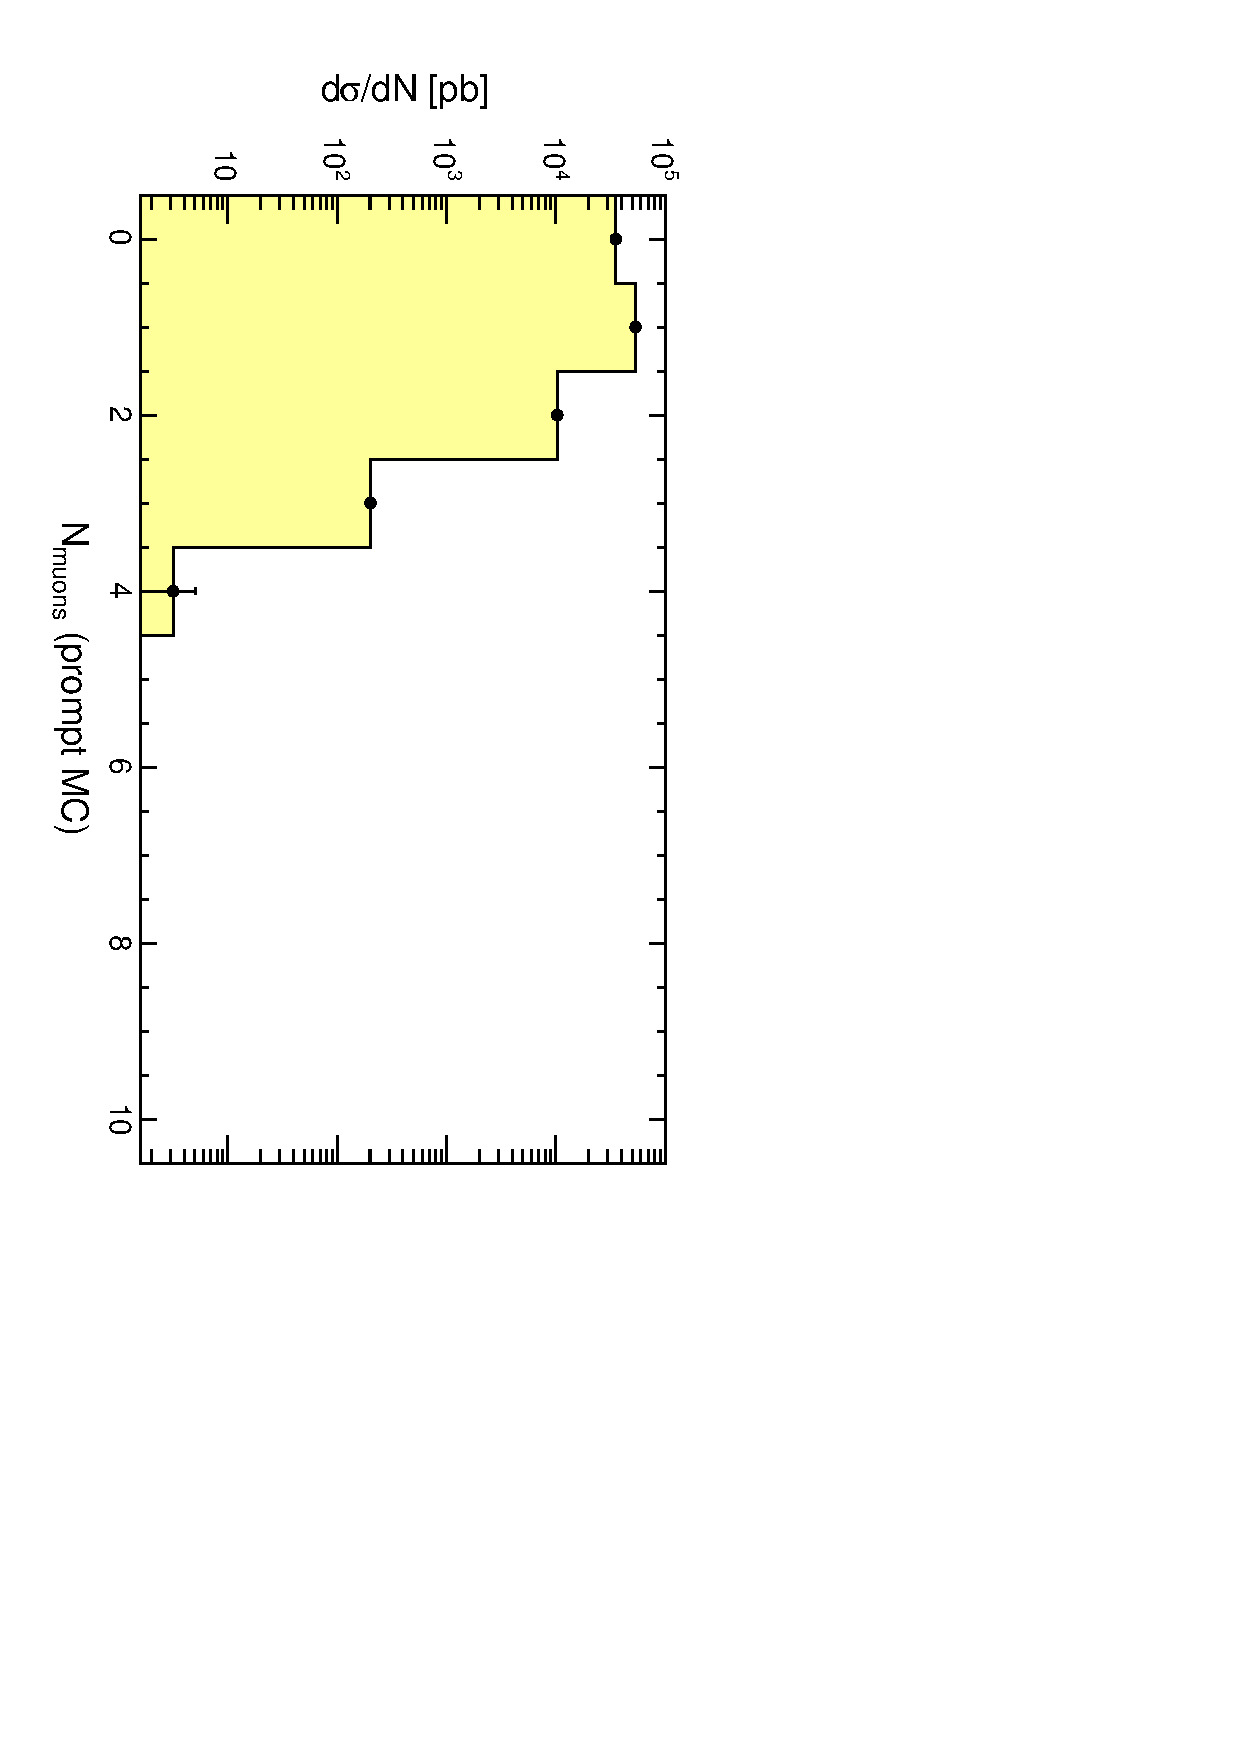
\includegraphics[height=0.5\linewidth, angle=90]{nmuons_real_NoMatching.pdf}
\end{frame}

\begin{frame}
\frametitle{Misreconstruction backgrounds}

\begin{itemize}
\item Out-of-the-box TrackerMuons yield any track that might point to a muon segment: a huge over-estimate (even including $p_T > 5$~GeV/$c$)
\item Track quality cuts can help: which are the most important?
\item Plot $N_\s{reco}$ for each number of $N_\s{real}$ and a general $N_\s{reco}$ distribution;
$N_\s{real}$ is defined using method \#1 (unique MC-matching)
\end{itemize}

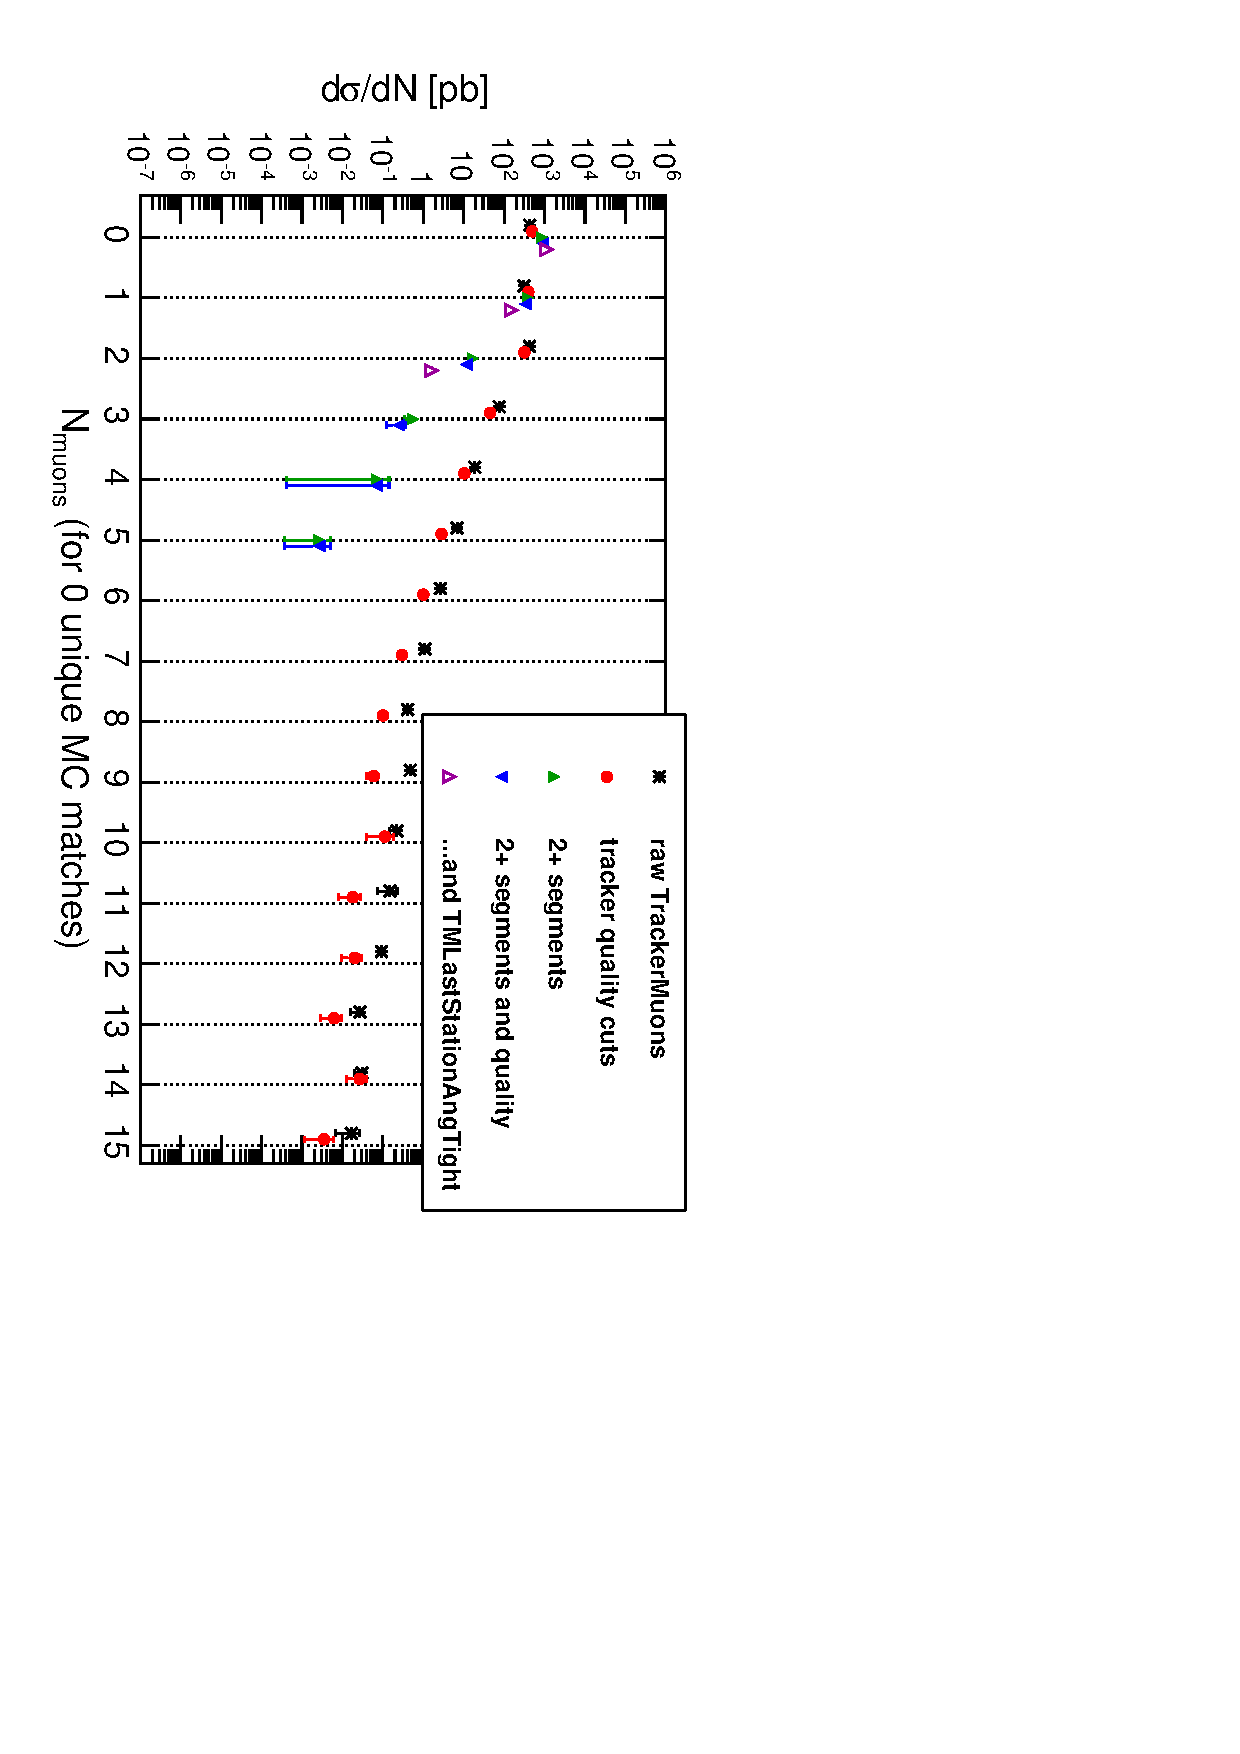
\includegraphics[height=0.45\linewidth, angle=90]{tracks_cuts_0real.pdf}
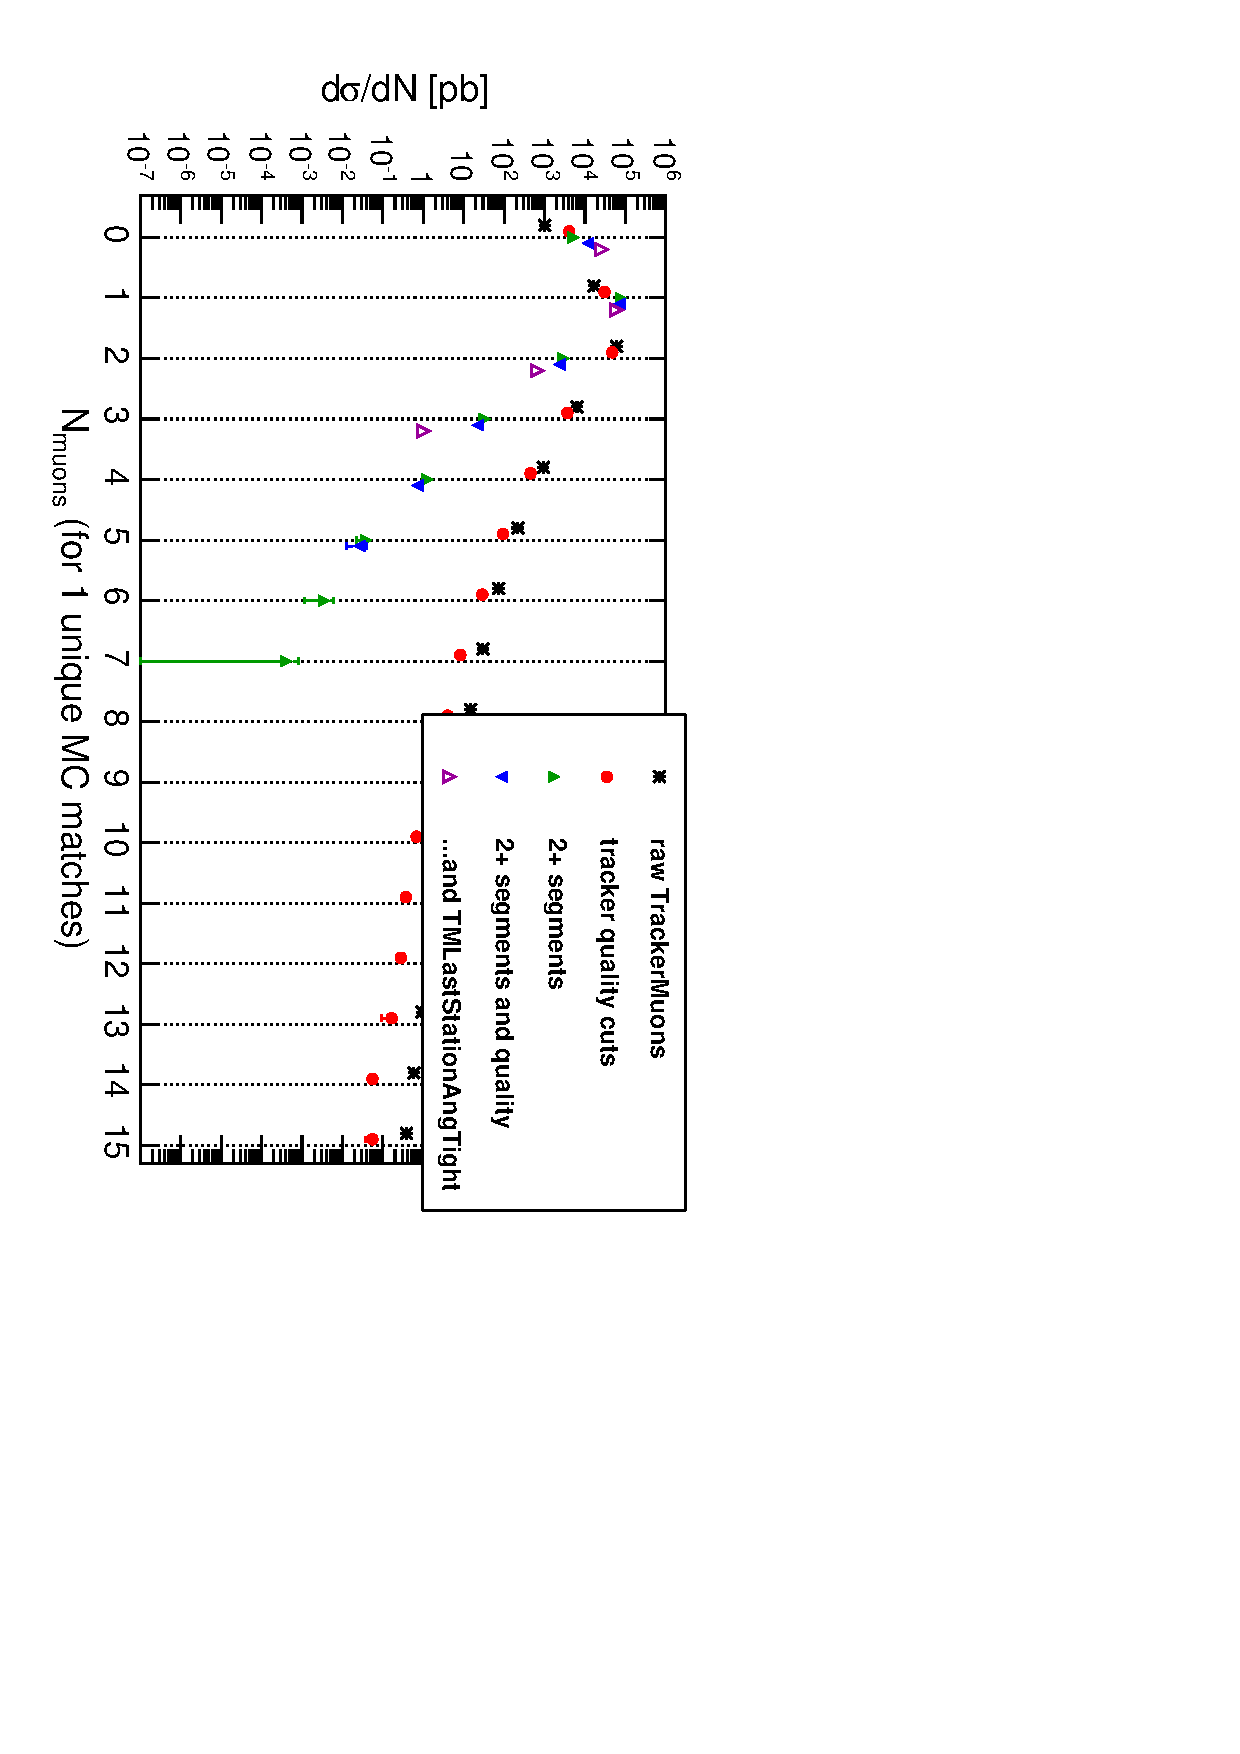
\includegraphics[height=0.45\linewidth, angle=90]{tracks_cuts_1real.pdf}

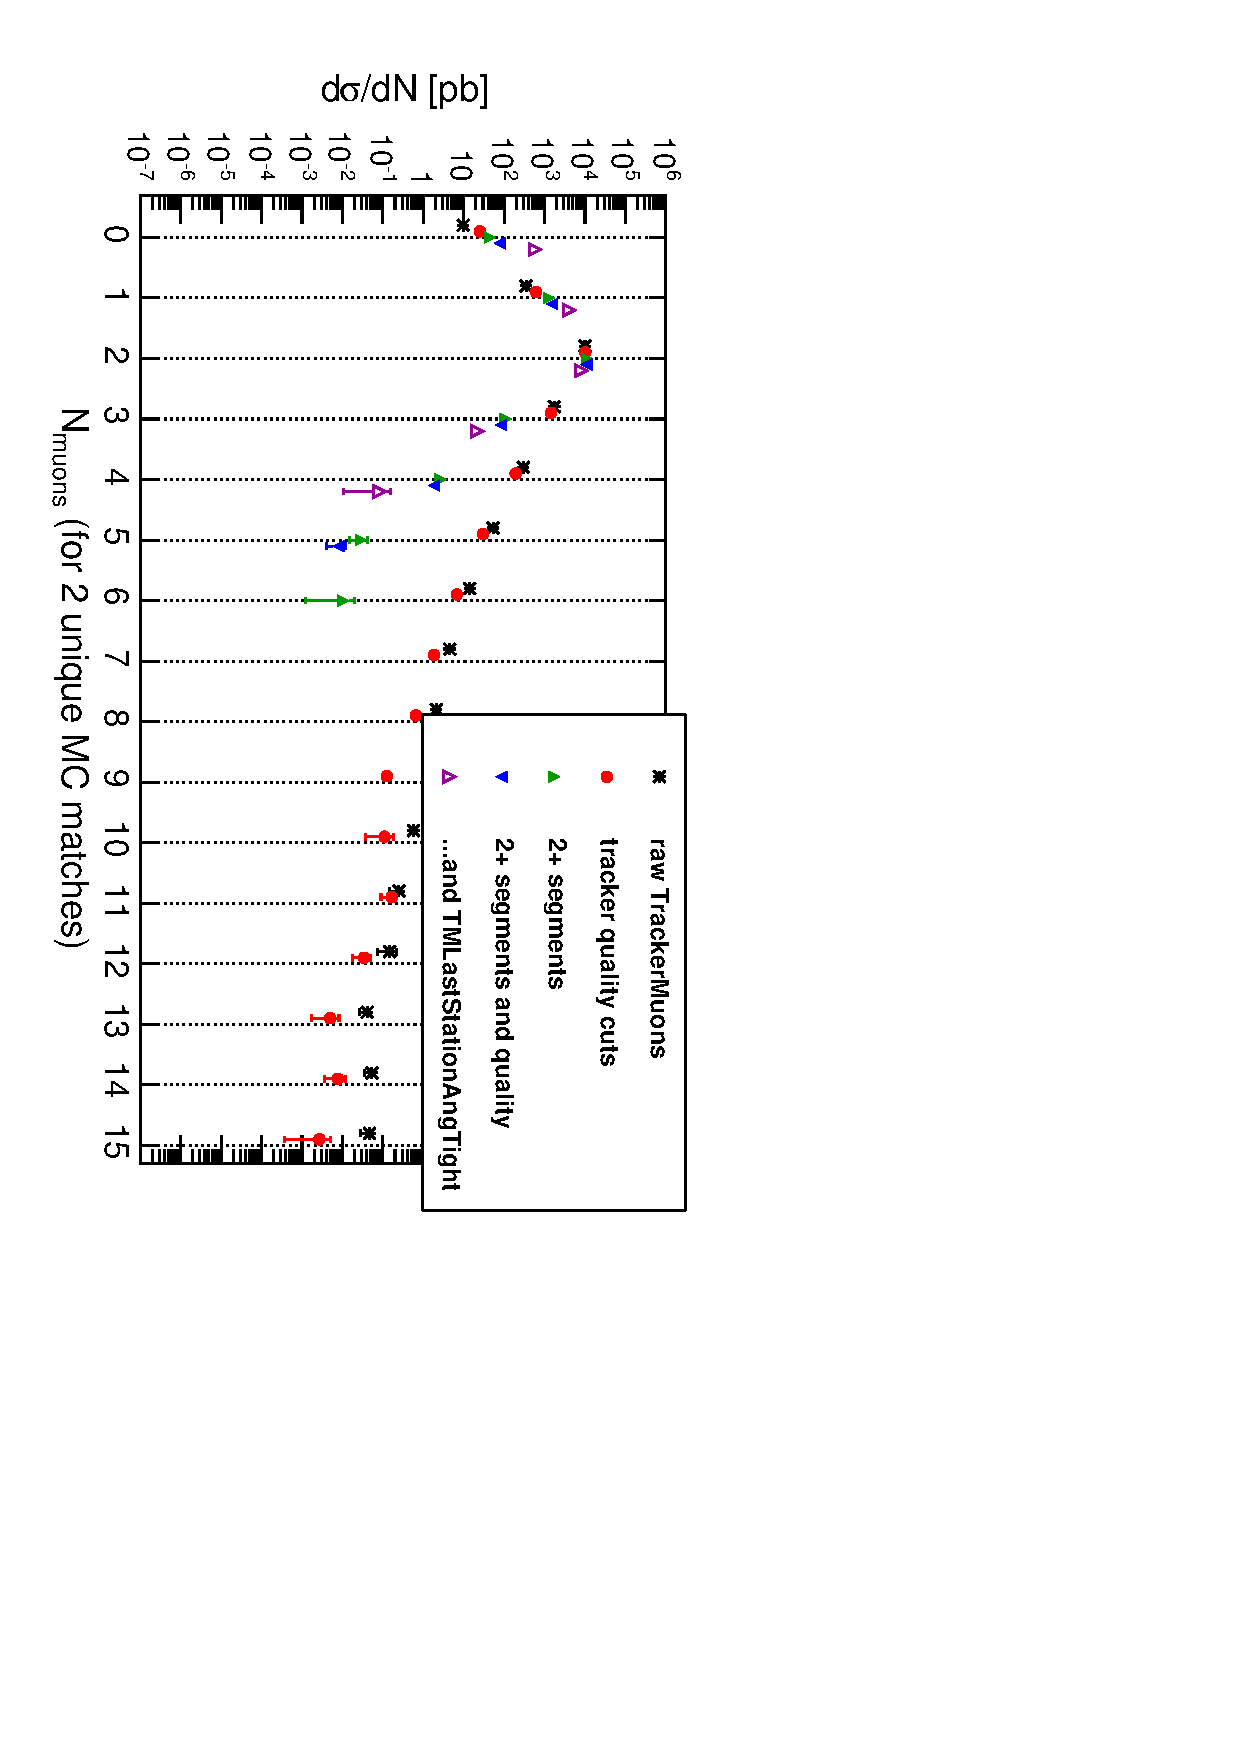
\includegraphics[height=0.45\linewidth, angle=90]{tracks_cuts_2real.pdf}
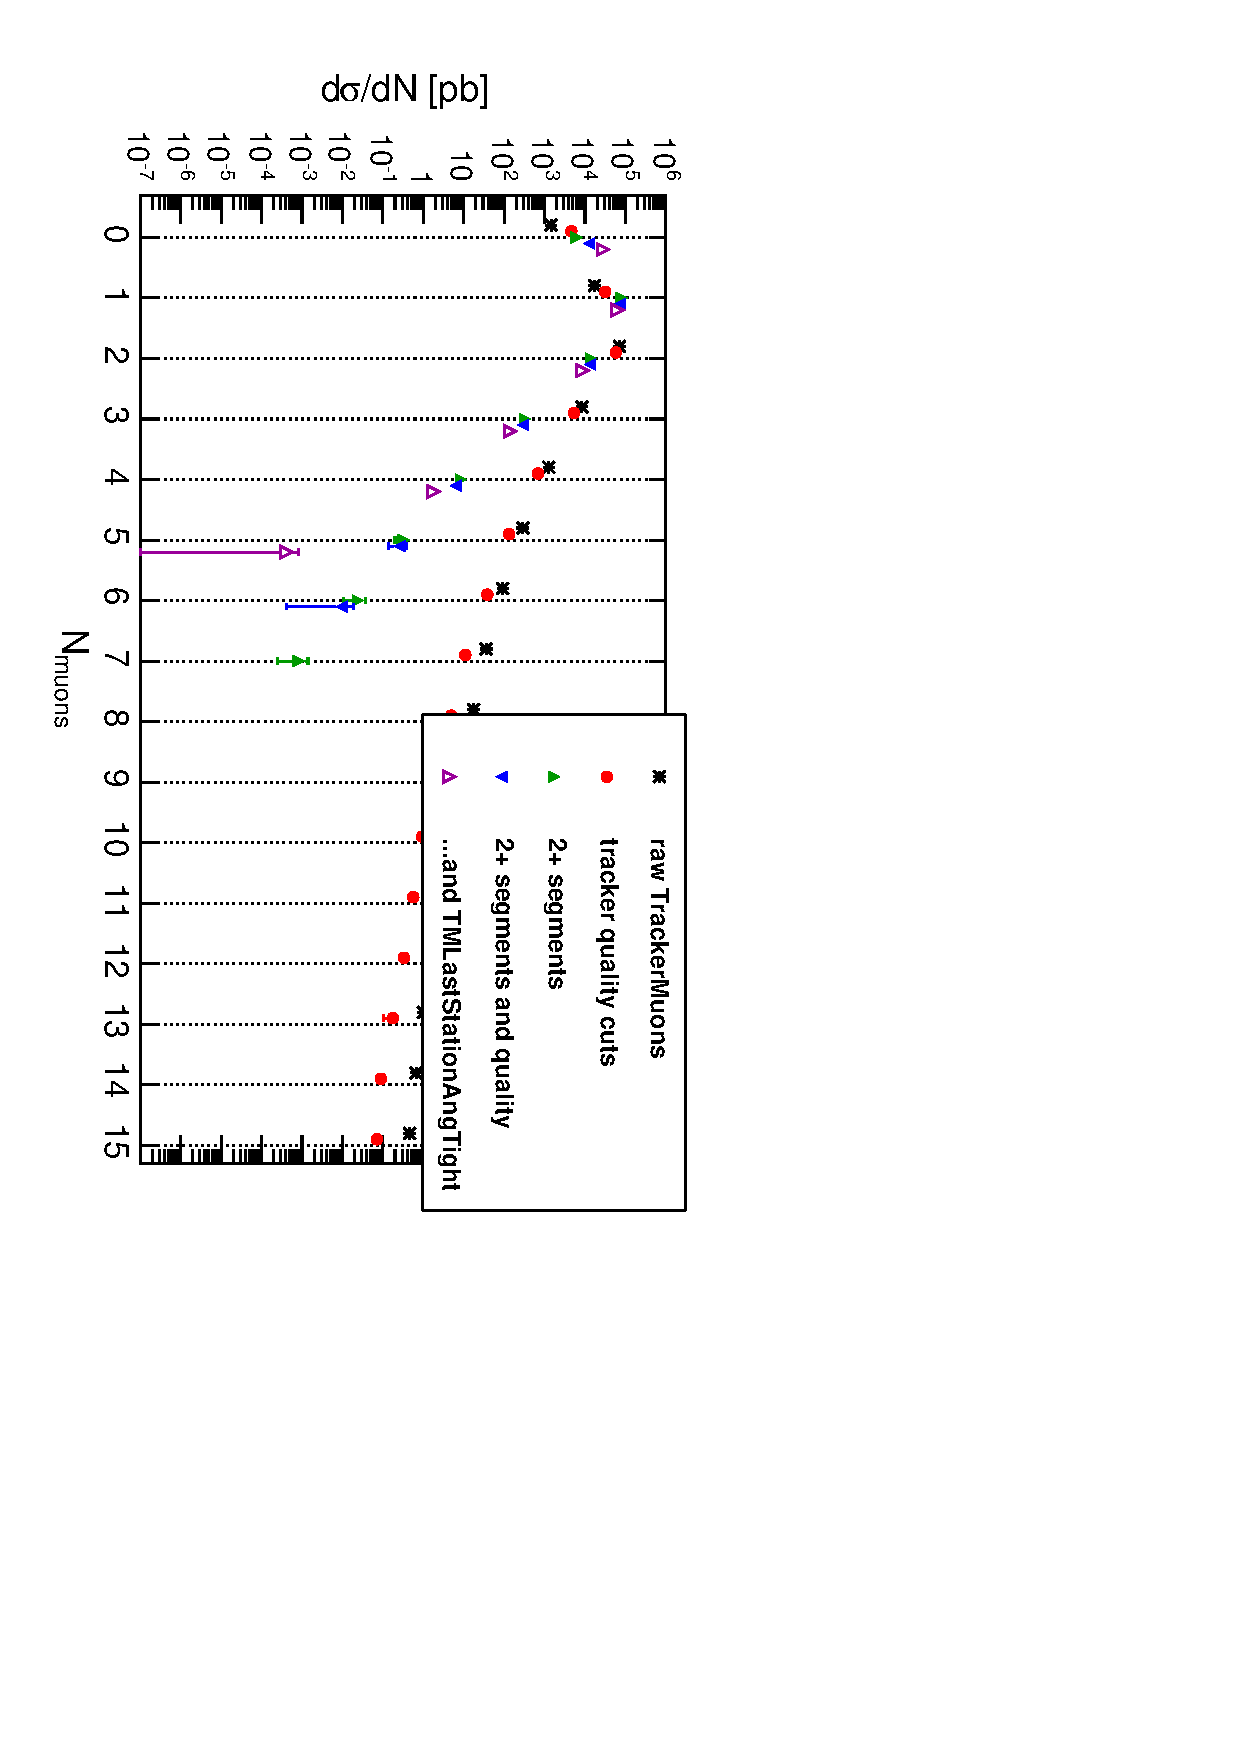
\includegraphics[height=0.45\linewidth, angle=90]{tracks_cuts_allreal.pdf}
\end{frame}

\begin{frame}
\frametitle{Misreconstruction backgrounds}

\begin{itemize}
\item Standard muon-POG selectors have similar background rejection, but lower efficiencies (not shown here)
\end{itemize}

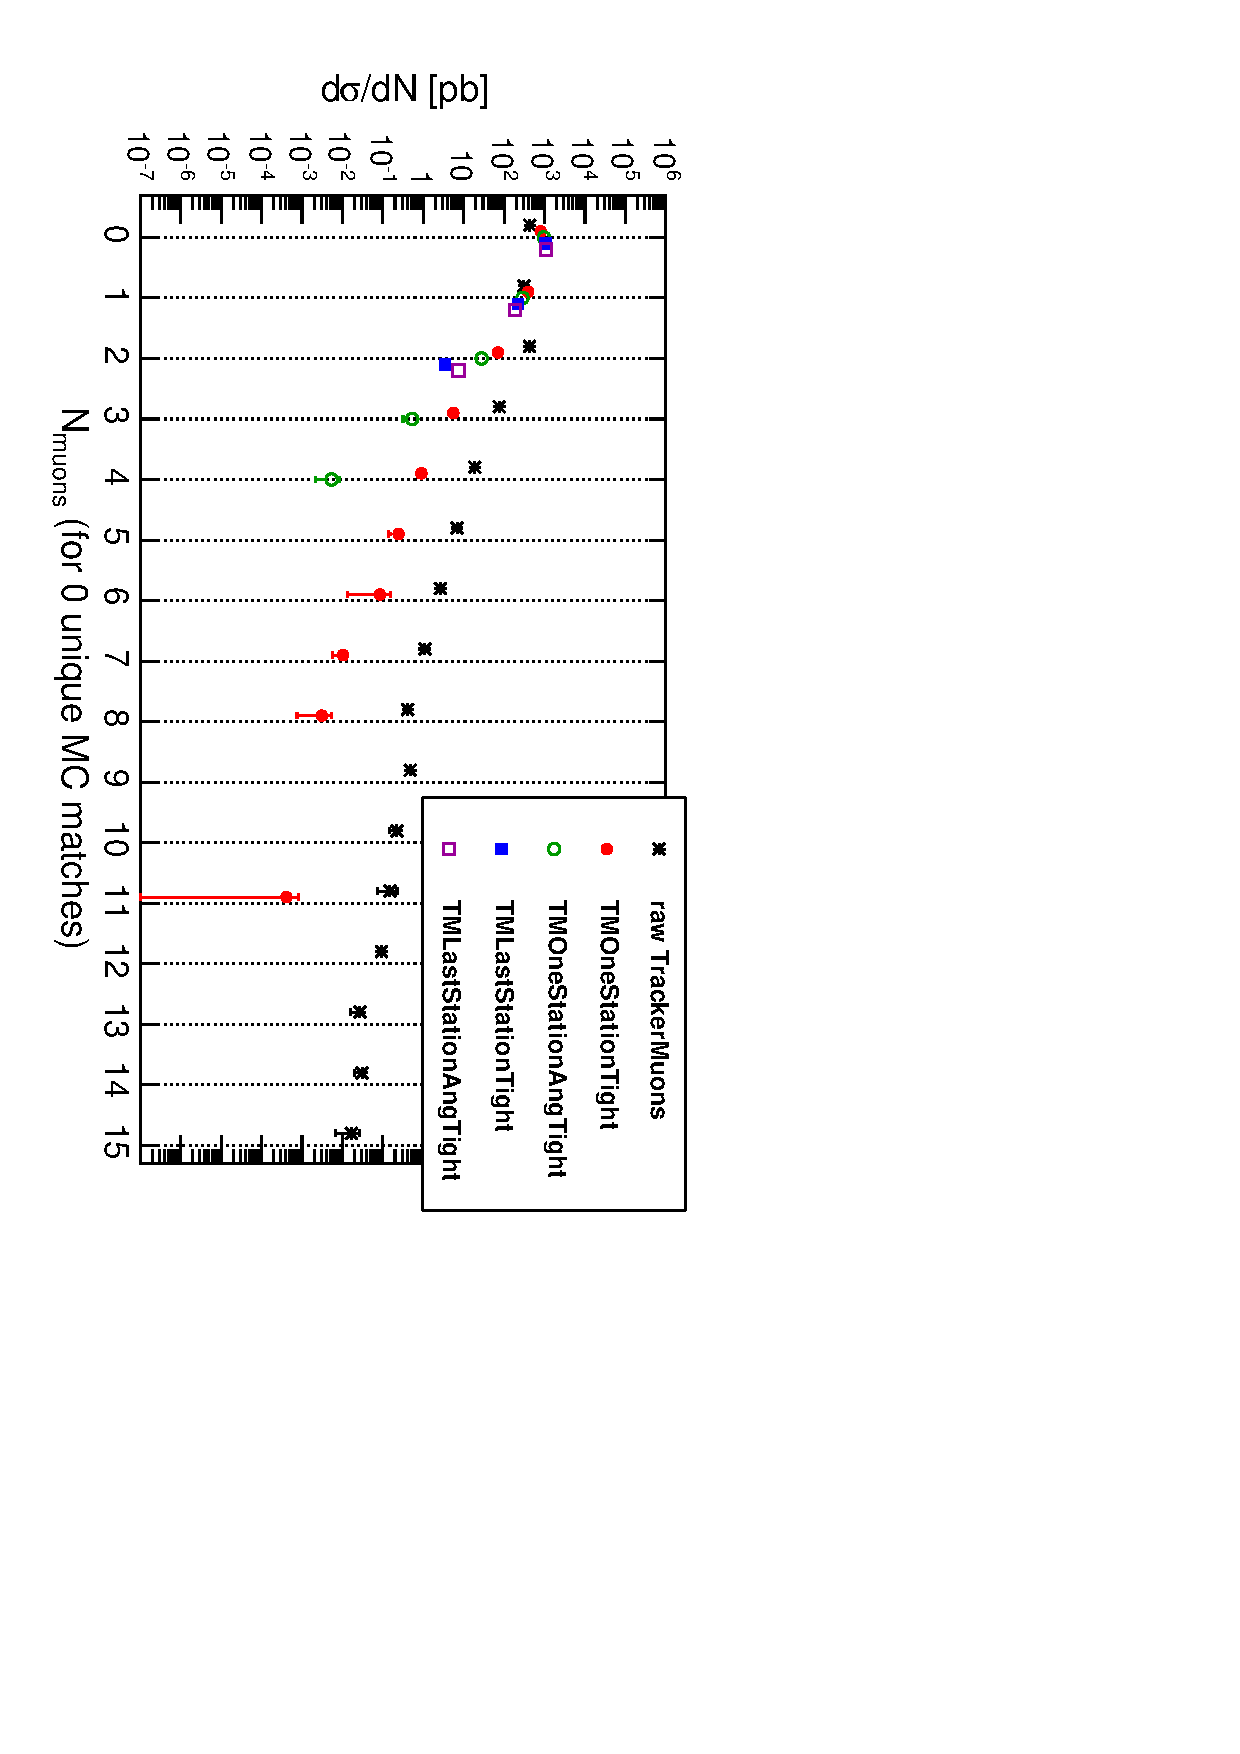
\includegraphics[height=0.45\linewidth, angle=90]{tracks_selectors_0real.pdf}
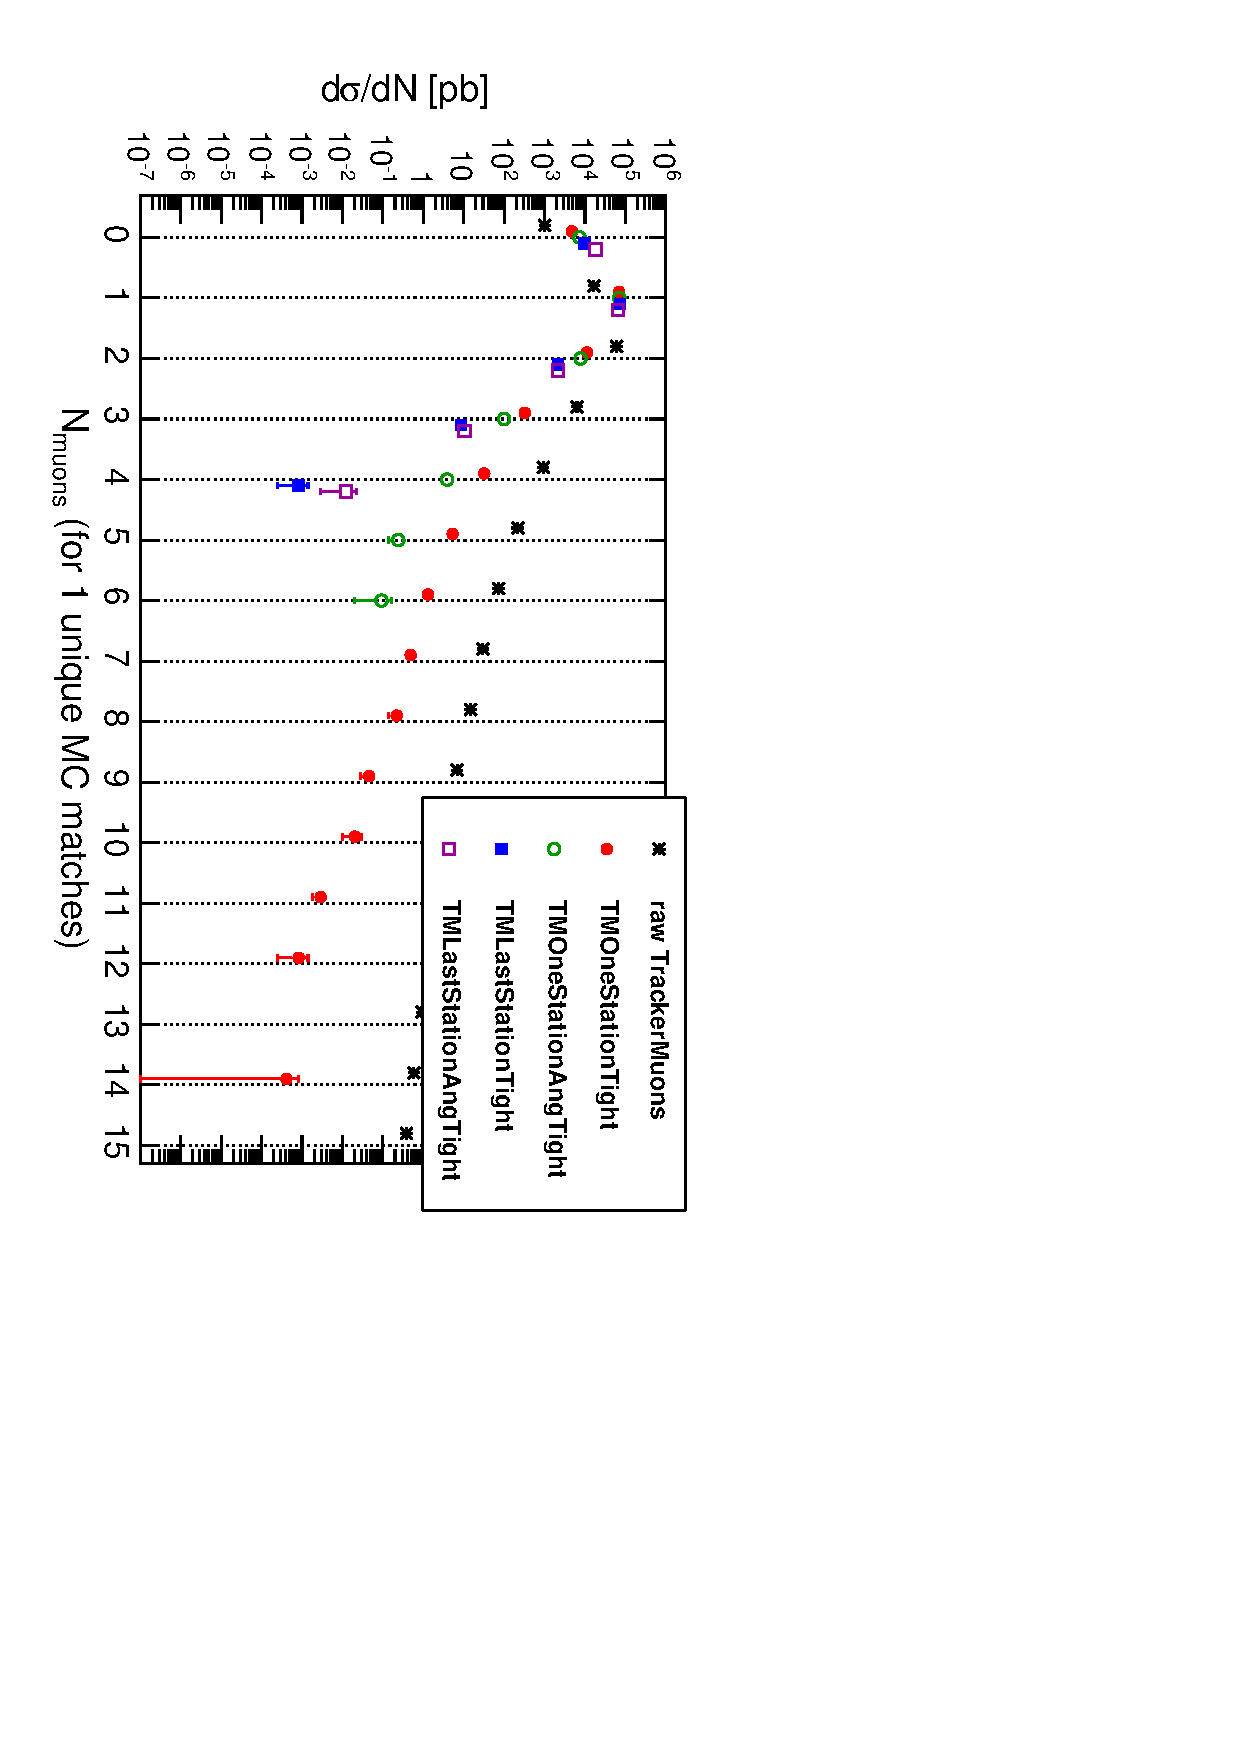
\includegraphics[height=0.45\linewidth, angle=90]{tracks_selectors_1real.pdf}

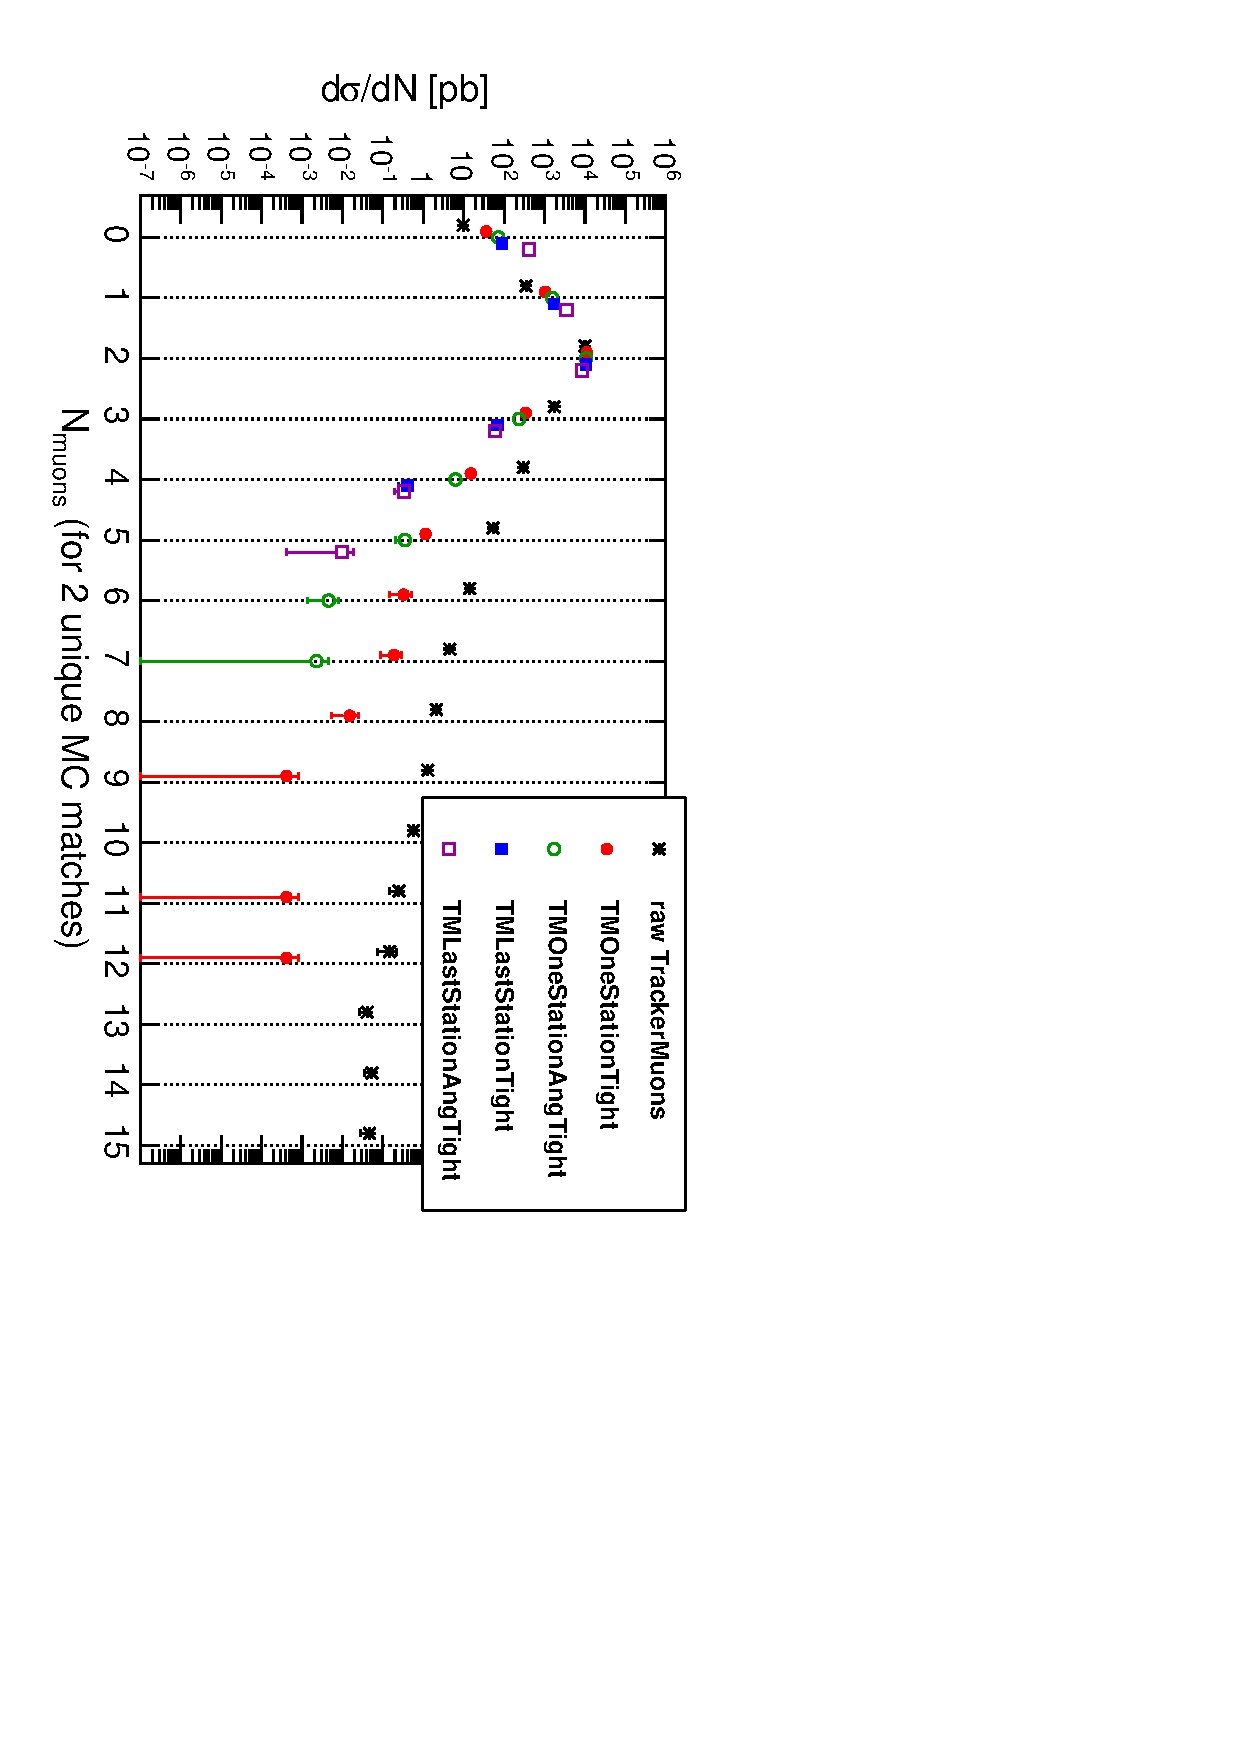
\includegraphics[height=0.45\linewidth, angle=90]{tracks_selectors_2real.pdf}
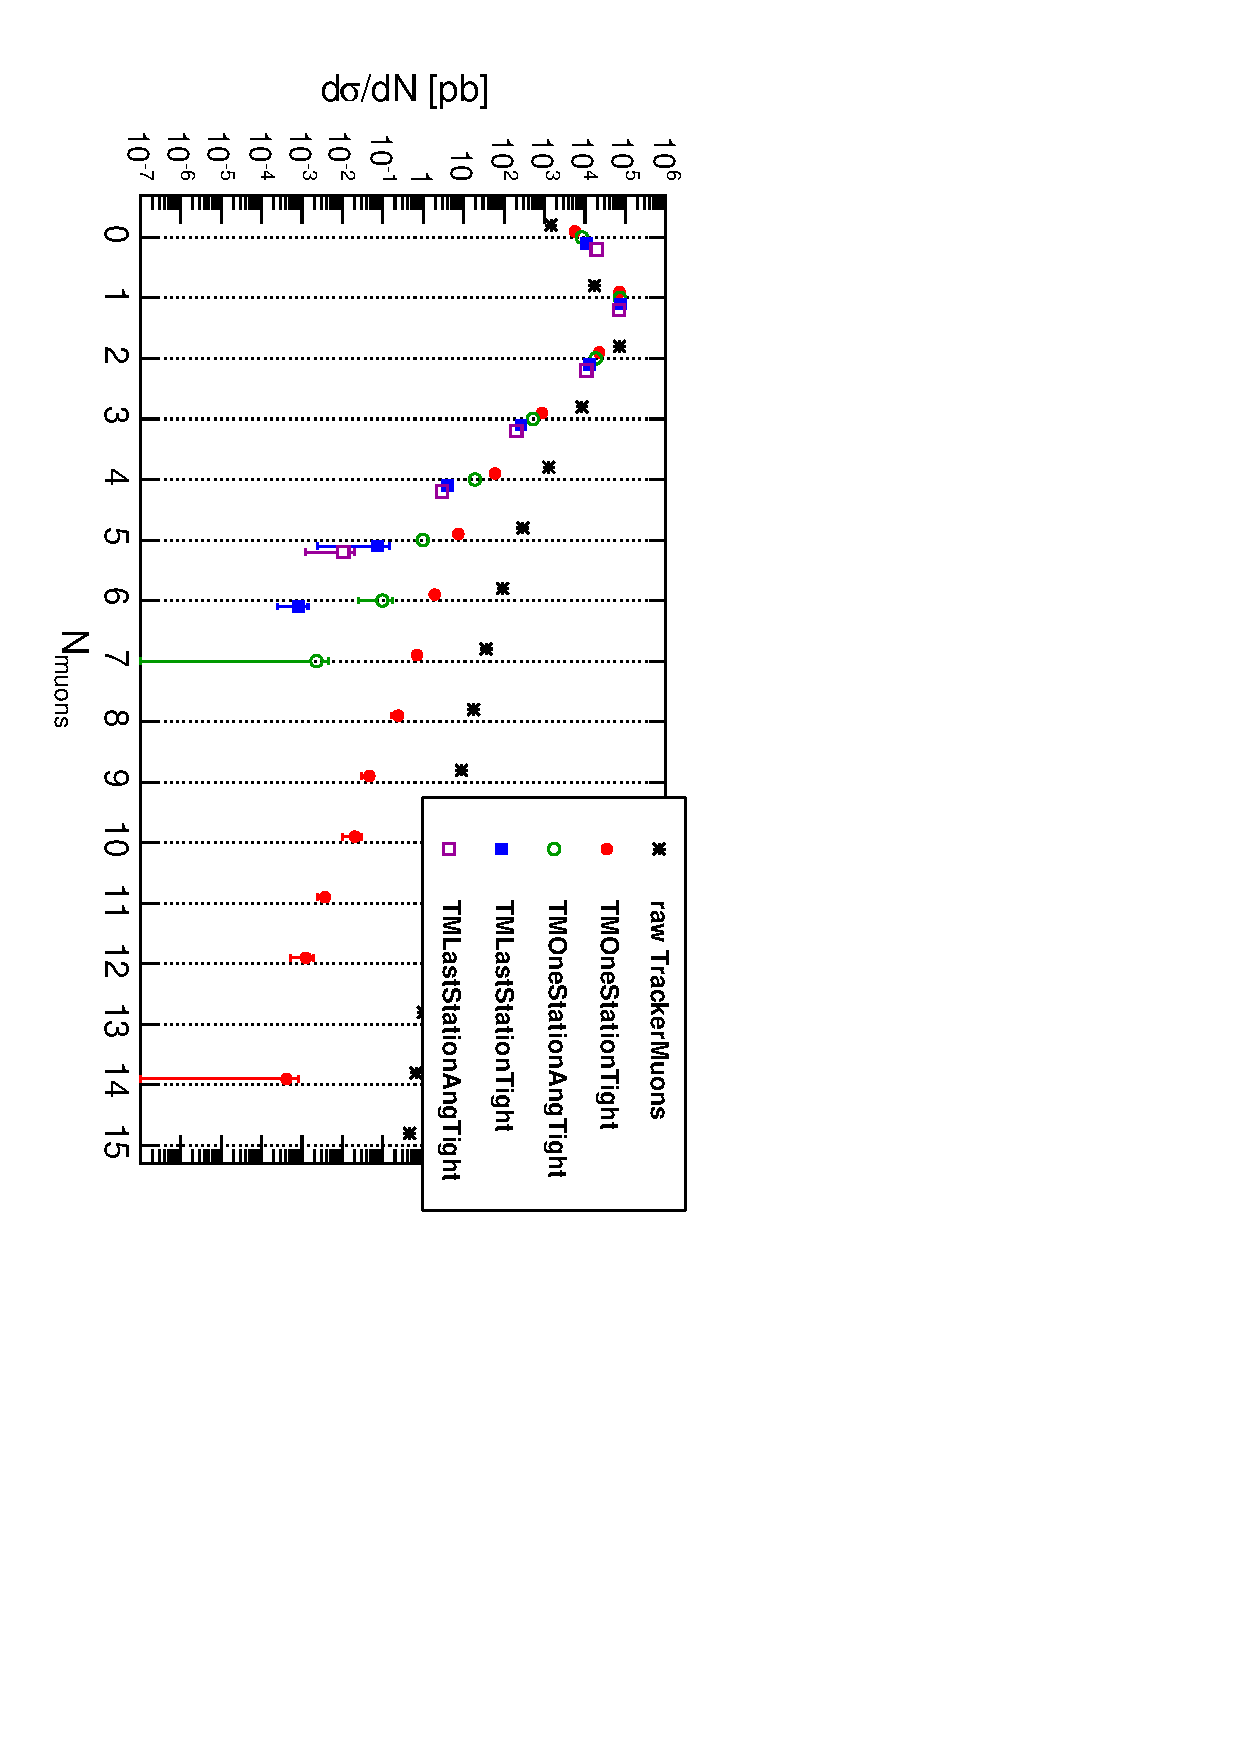
\includegraphics[height=0.45\linewidth, angle=90]{tracks_selectors_allreal.pdf}
\end{frame}

\begin{frame}
\frametitle{Misreconstruction backgrounds}

\begin{itemize}
\item GlobalMuons out-of-the-box are already near optimal, adding cuts doesn't help much
\item The tracker/standAlone normalized $\chi^2$ is consistency of
  tracker-track and StandAloneMuon (not guaranteed out-of-the-box)
\end{itemize}

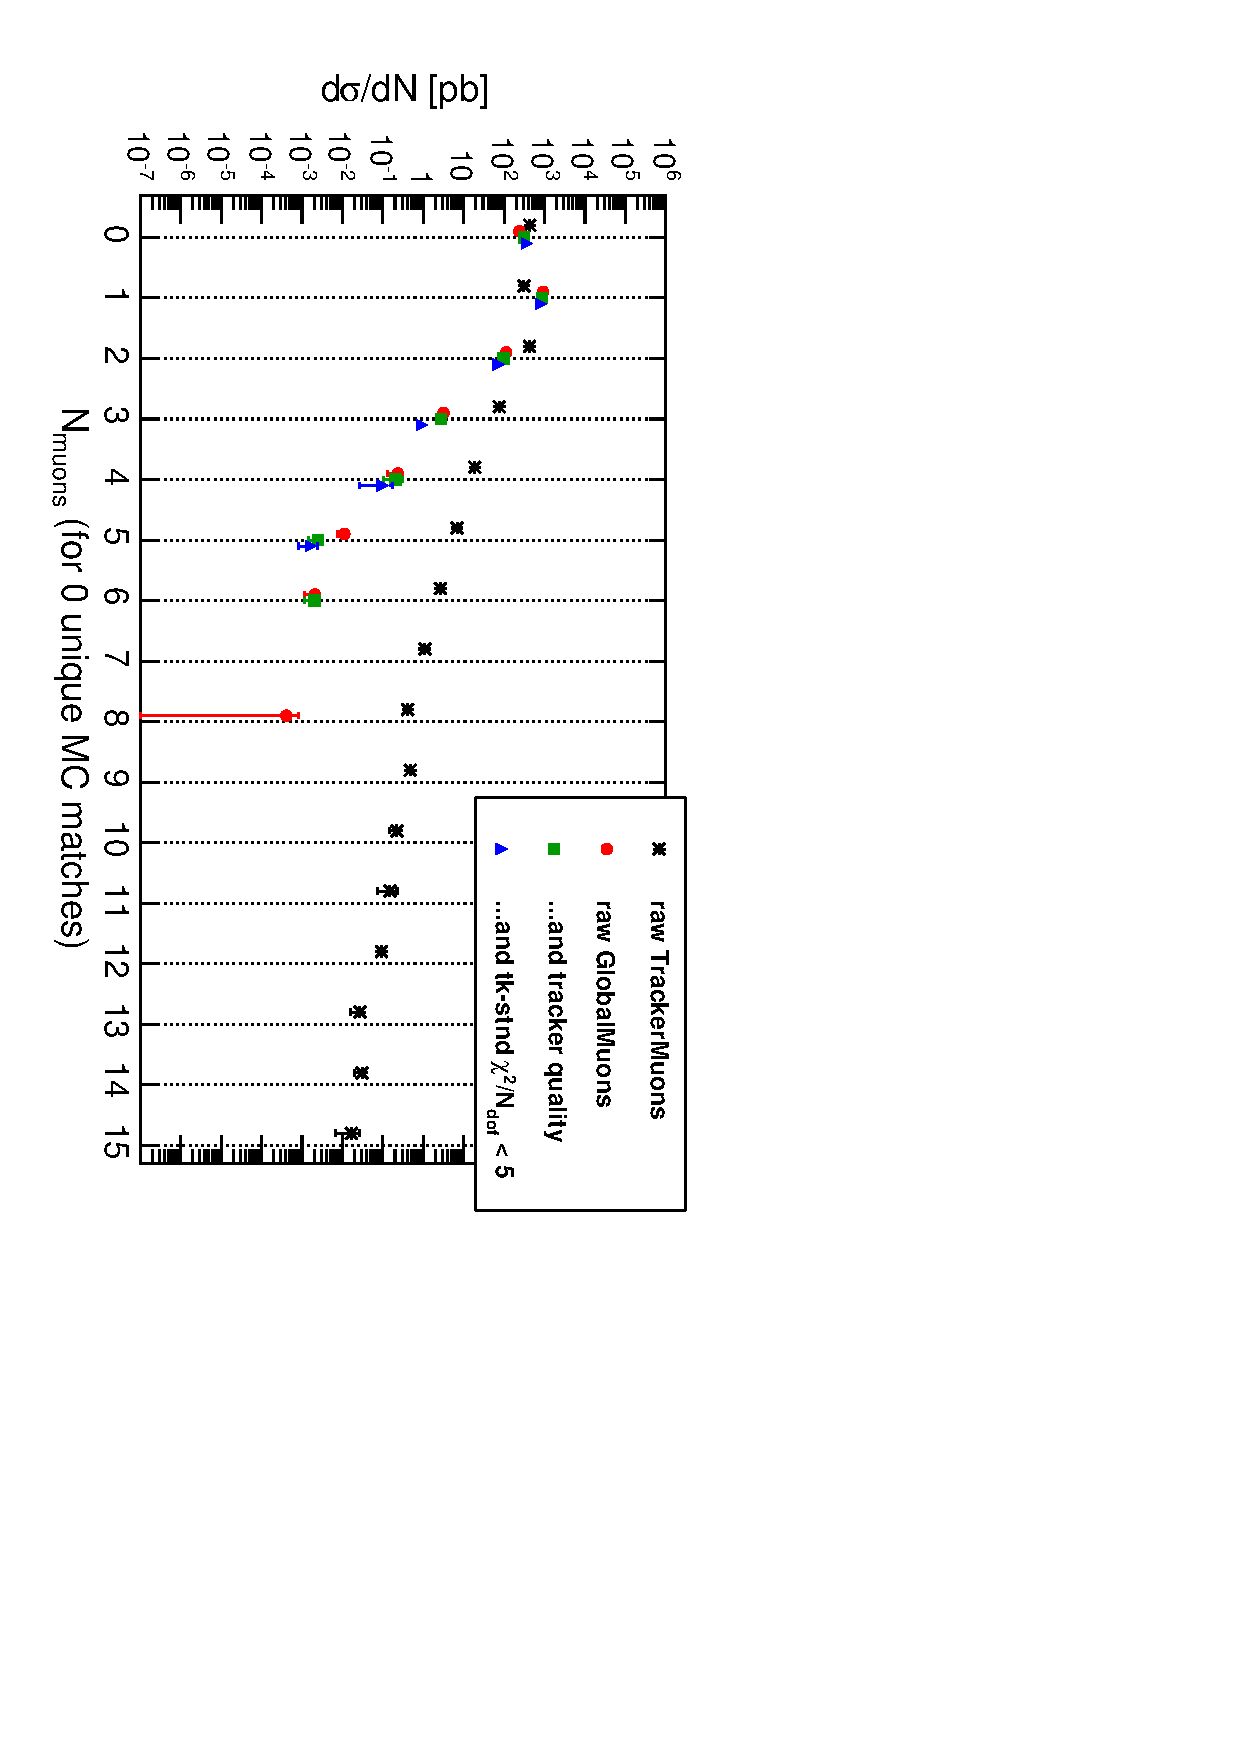
\includegraphics[height=0.45\linewidth, angle=90]{tracks_global_0real.pdf}
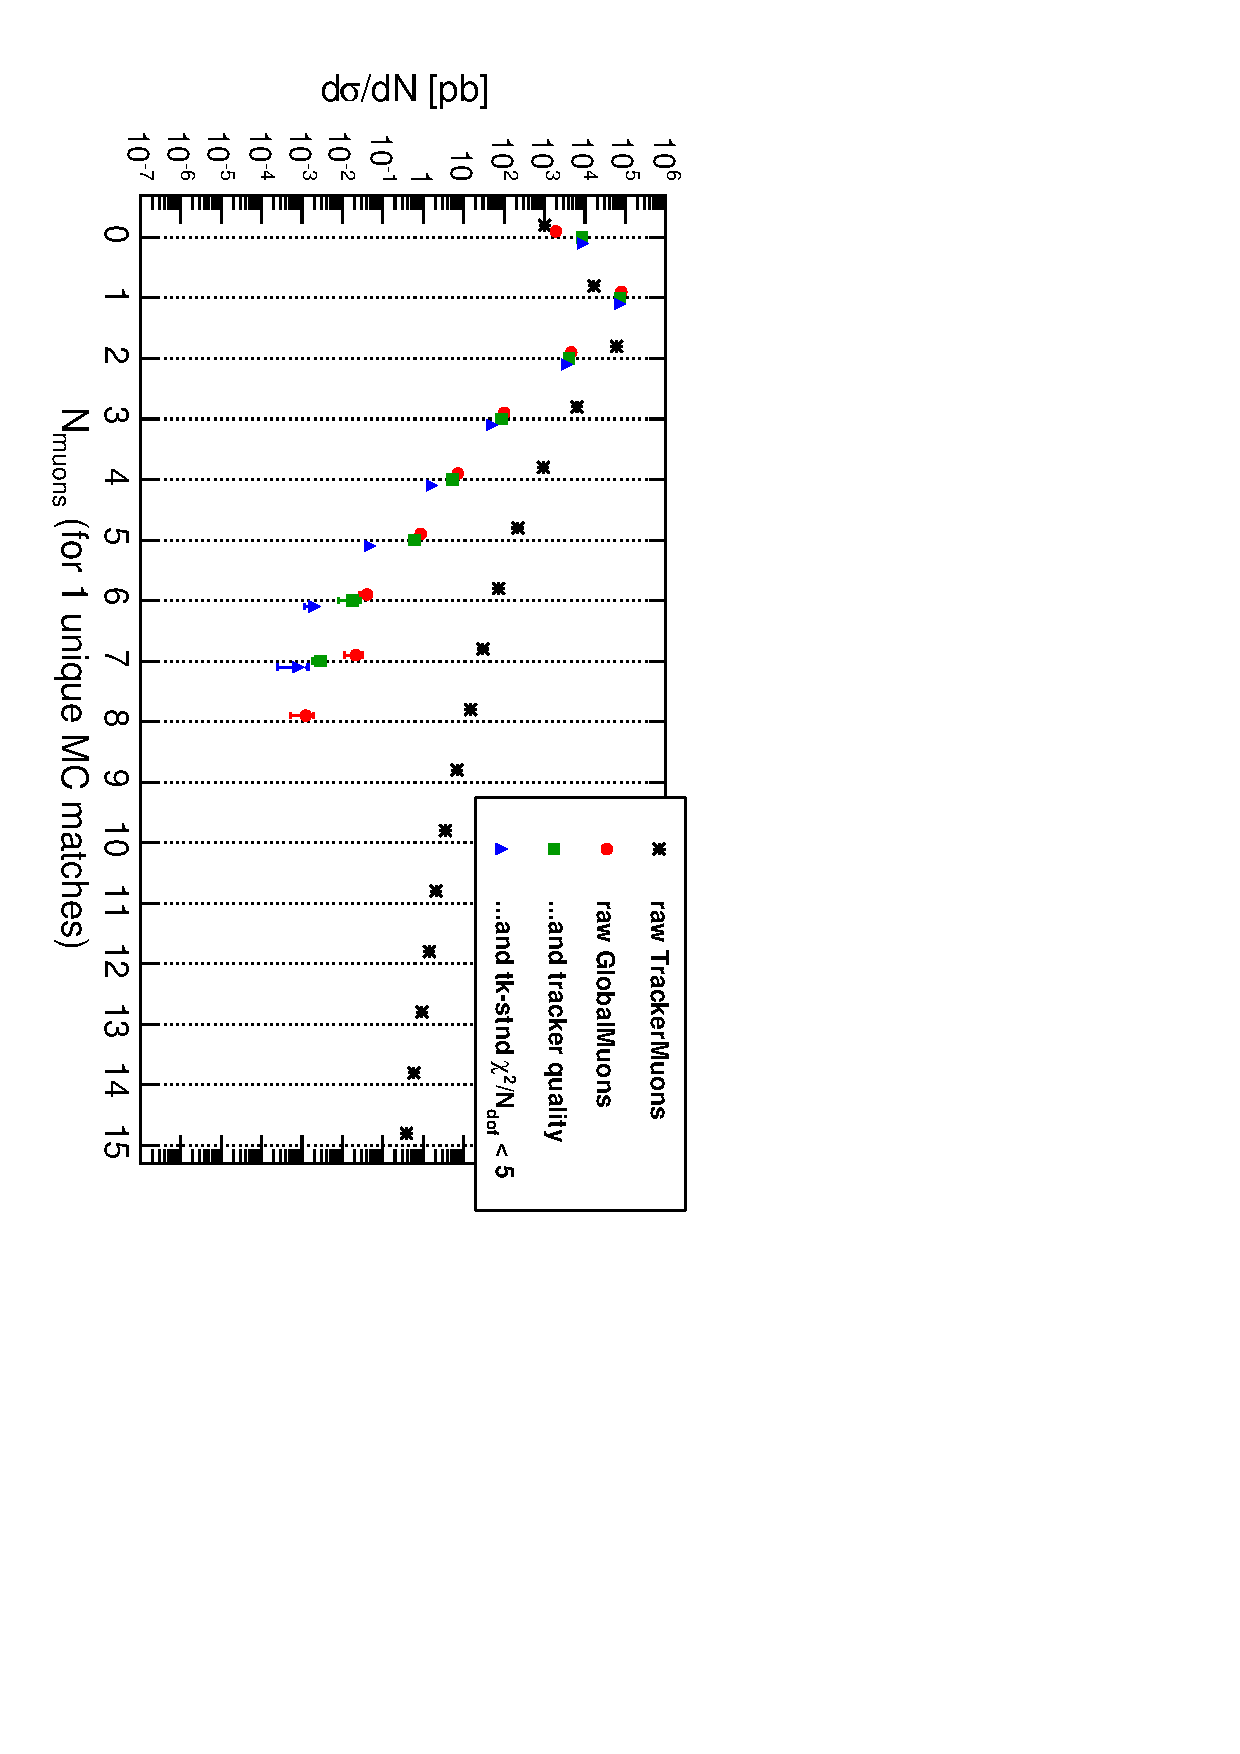
\includegraphics[height=0.45\linewidth, angle=90]{tracks_global_1real.pdf}

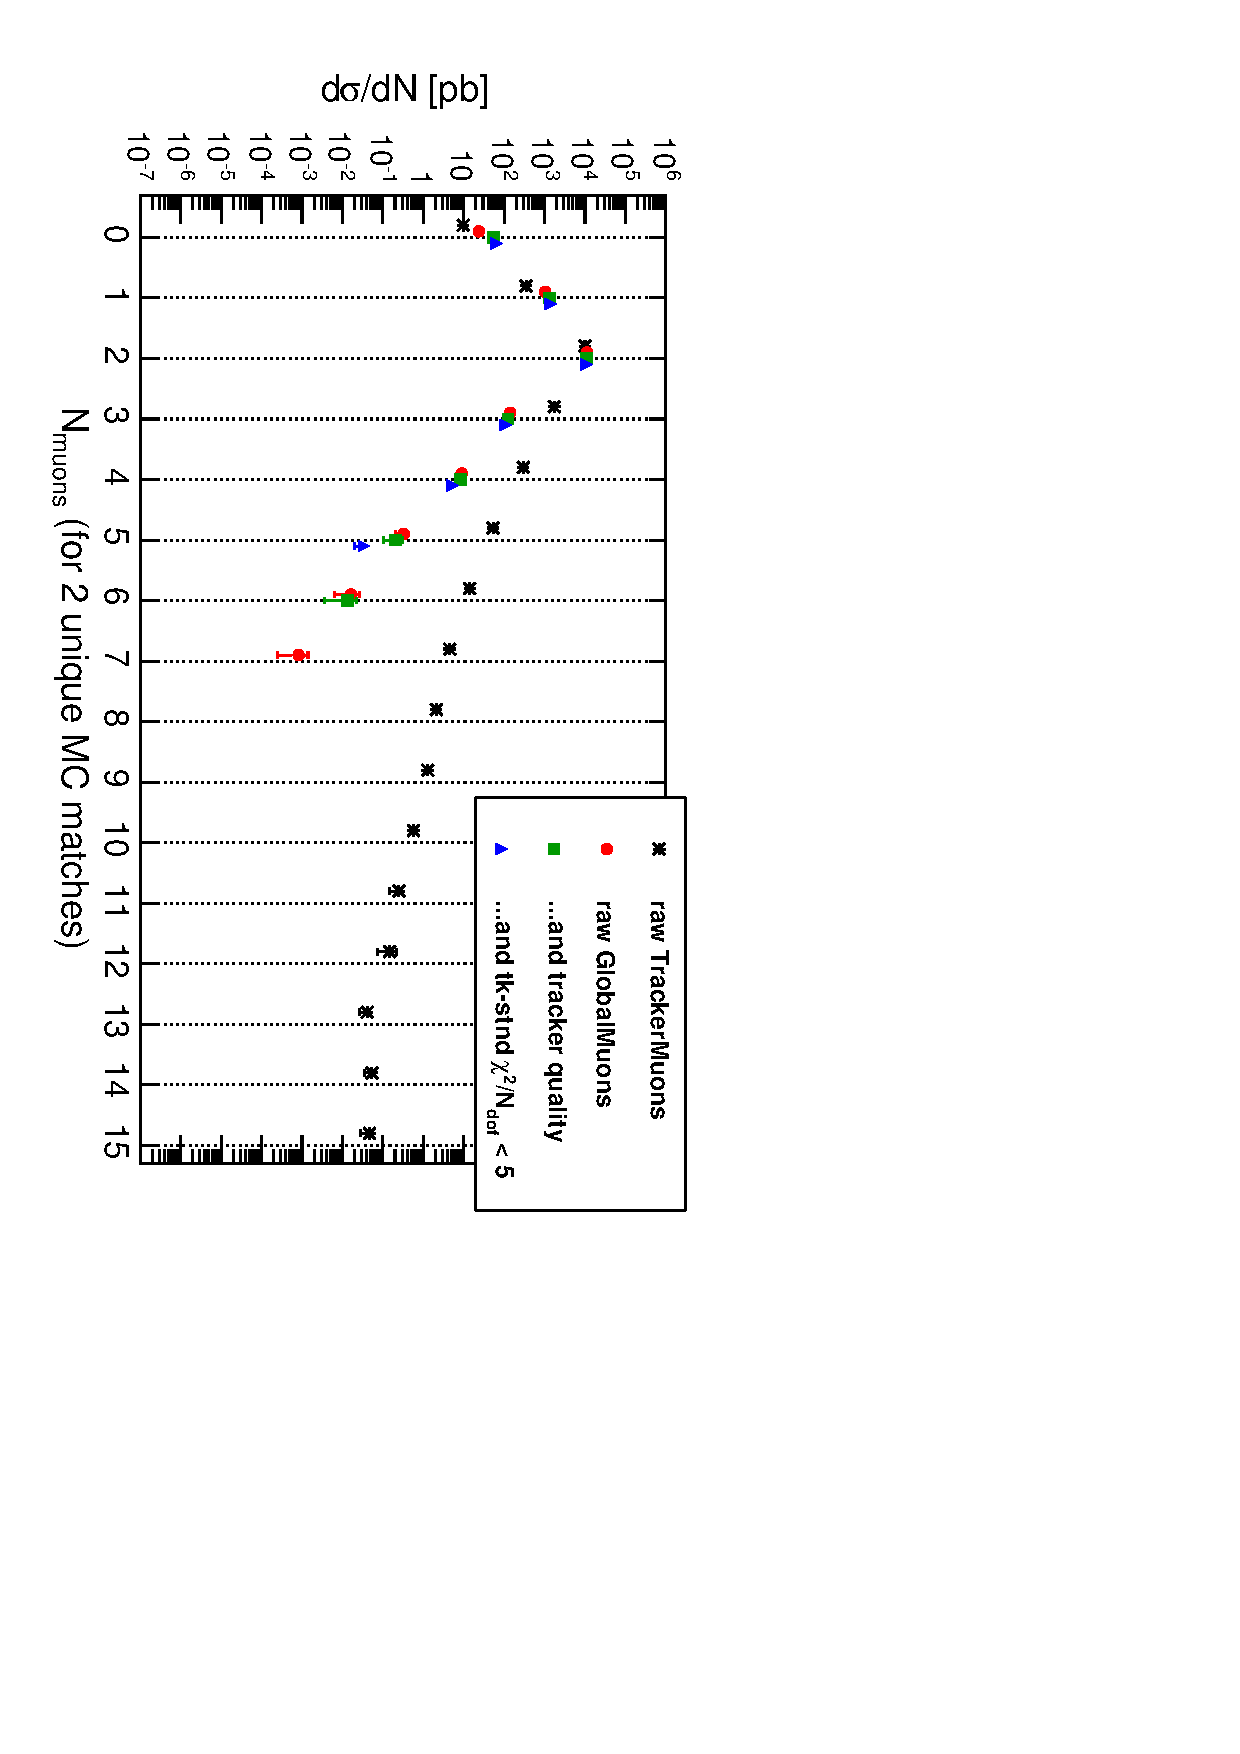
\includegraphics[height=0.45\linewidth, angle=90]{tracks_global_2real.pdf}
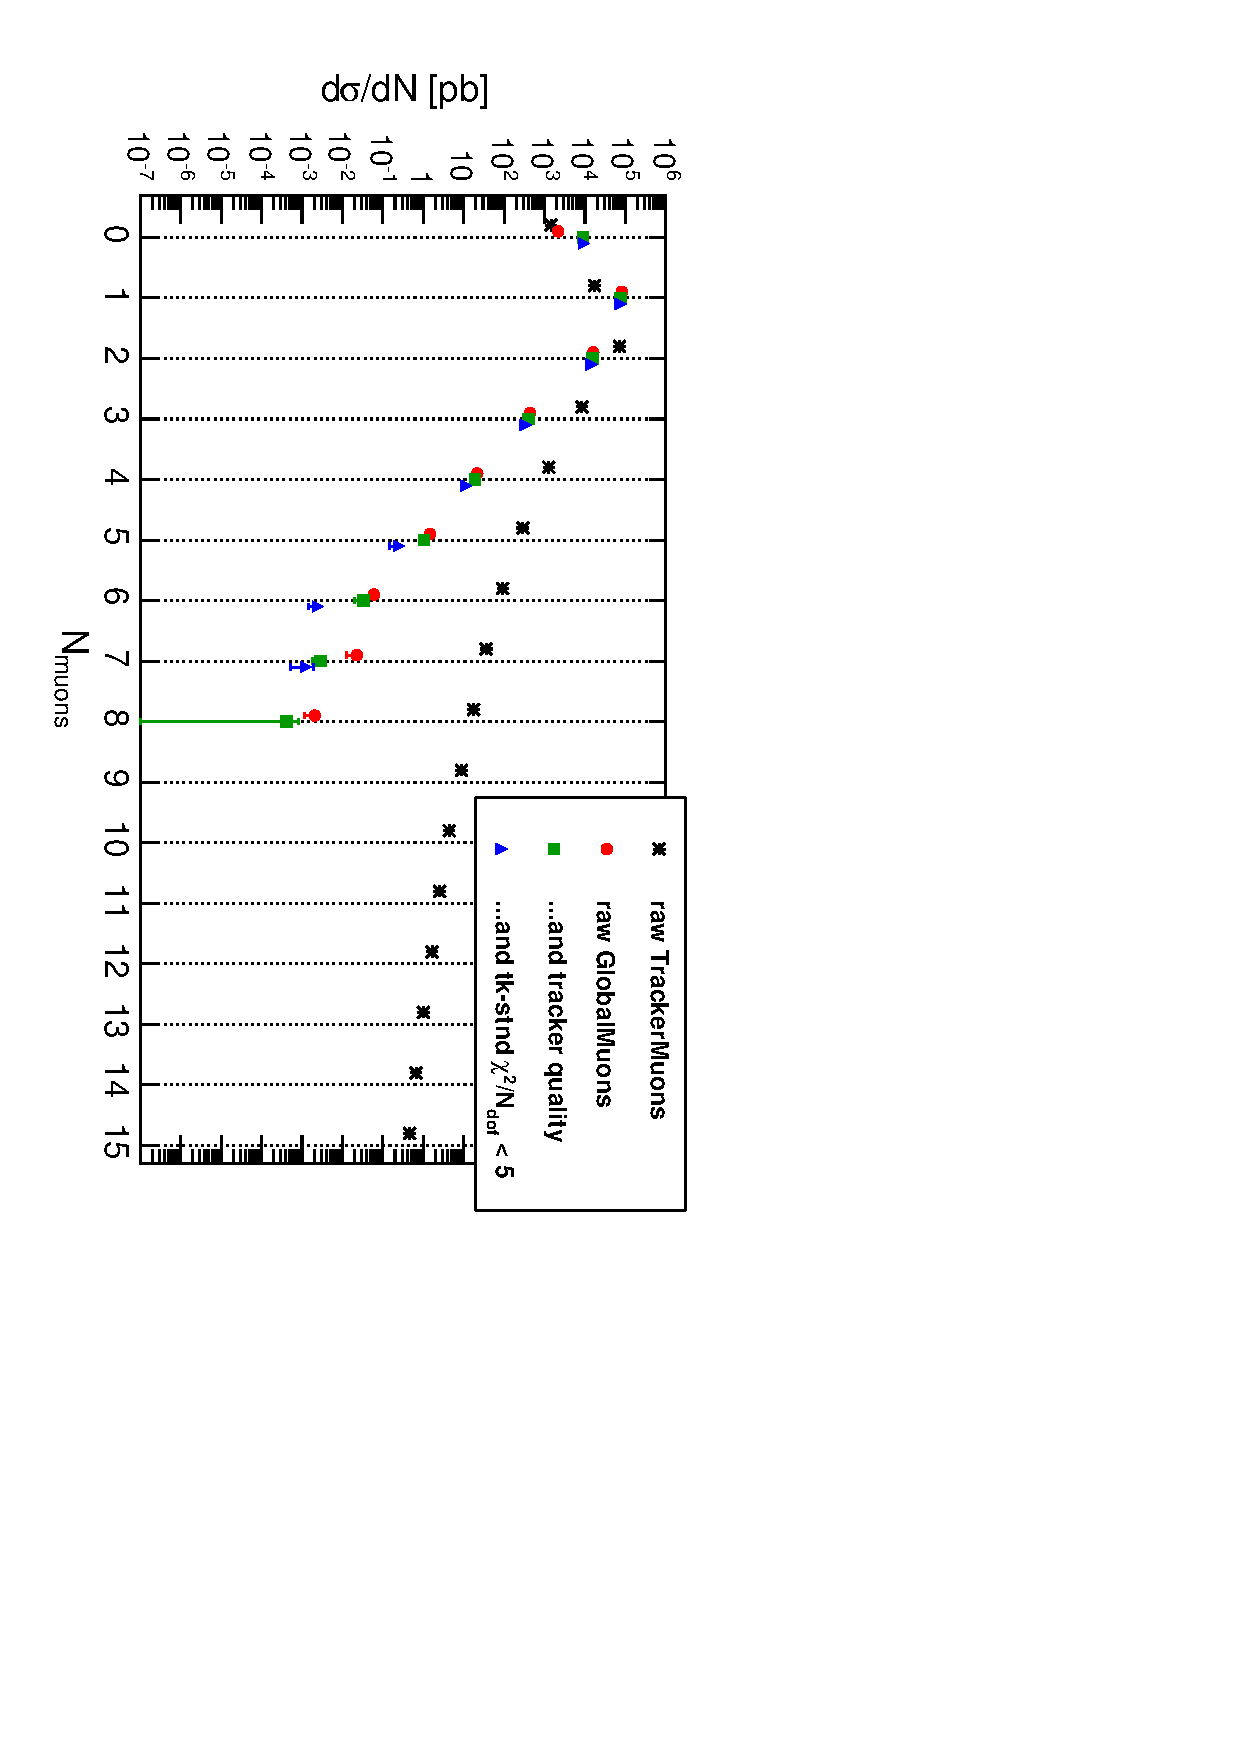
\includegraphics[height=0.45\linewidth, angle=90]{tracks_global_allreal.pdf}
\end{frame}

\begin{frame}
\frametitle{Misreconstruction backgrounds}

\begin{itemize}
\item All on one page, for your convenience
\item From this point onward, I'm considering only
\begin{itemize}
\item raw TrackerMuons (straw-man)
\item quality TrackerMuons, including a $N_\s{segments} \ge 2$ requirement
\item raw GlobalMuons
\end{itemize}
\end{itemize}

\begin{columns}
\column{0.7\linewidth}
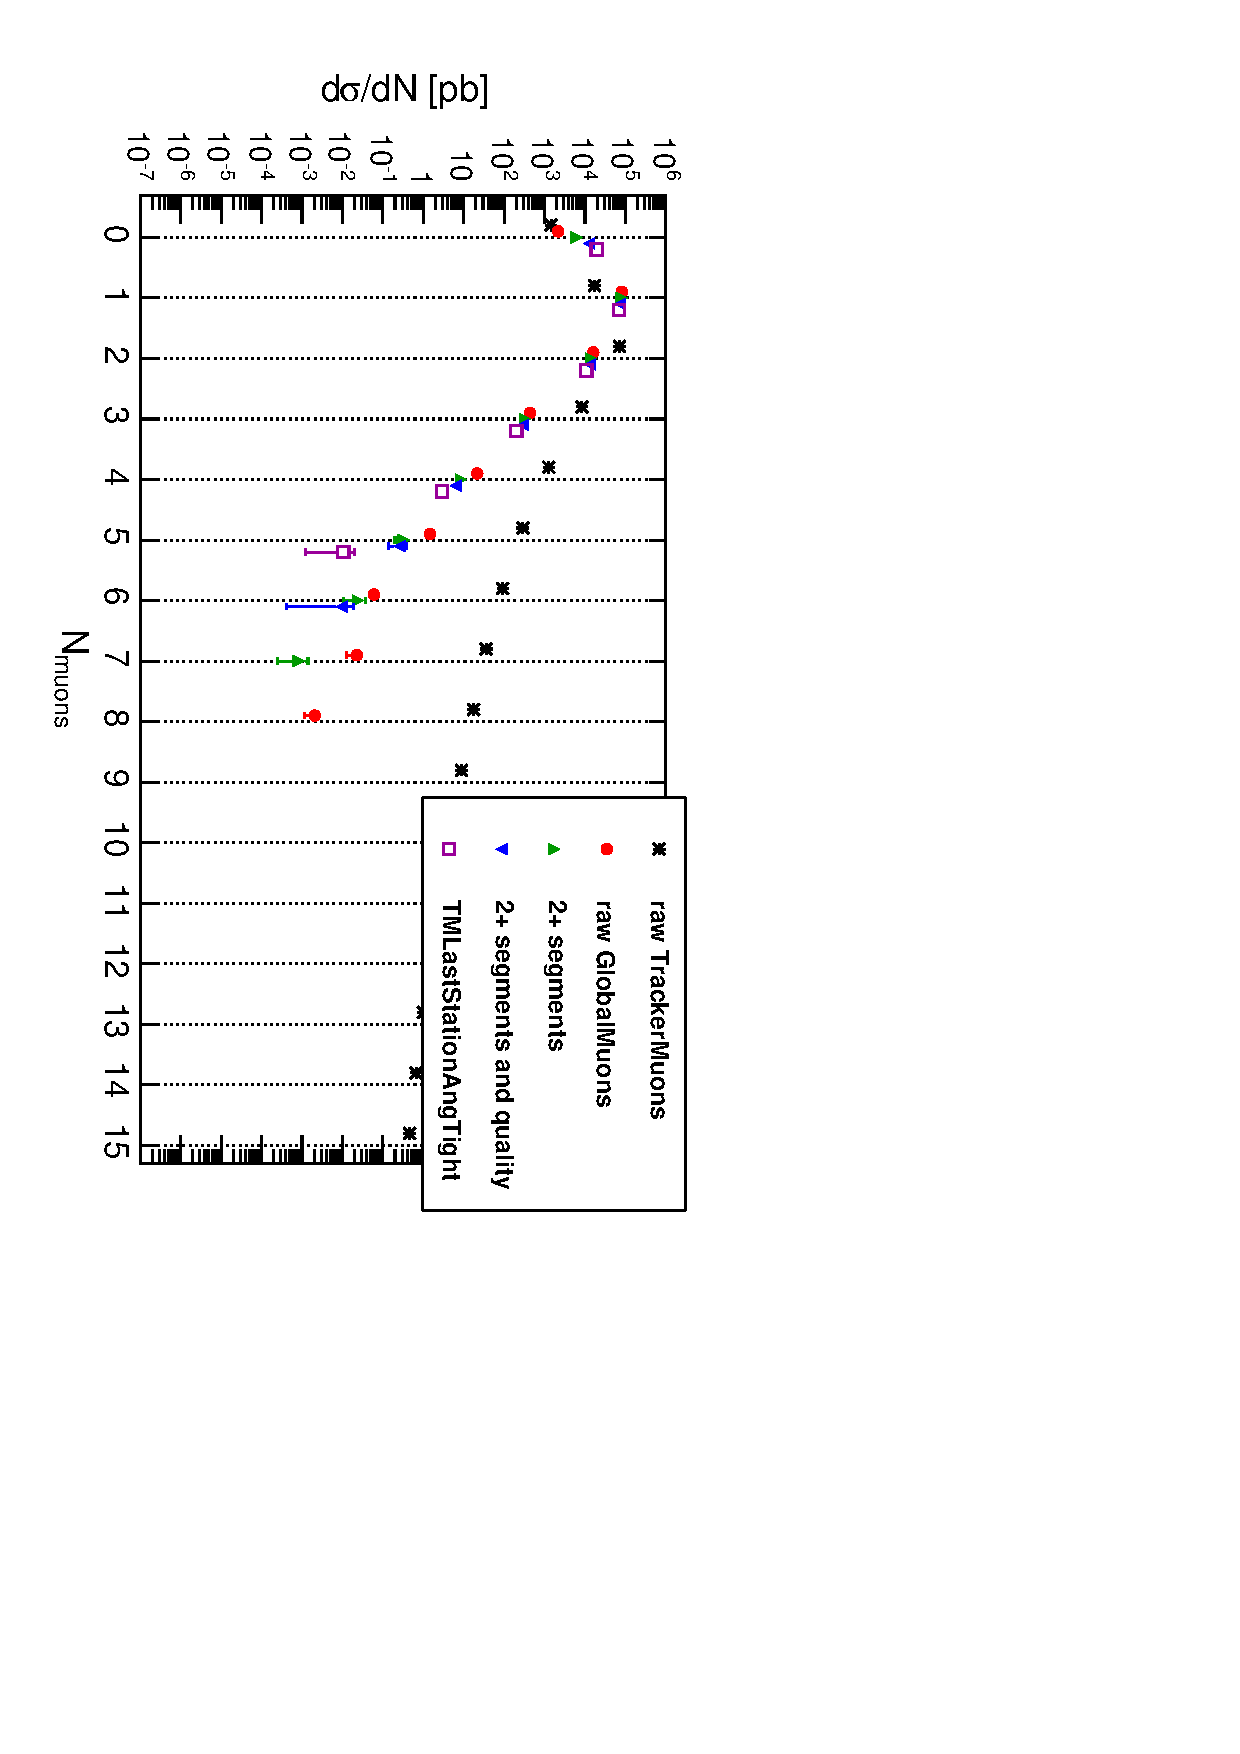
\includegraphics[height=\linewidth, angle=90]{tracks_samepage_allreal.pdf}

\column{0.3\linewidth}
\scriptsize ``Quality cuts'' are:

$N_\s{tracker hits} \ge 8$ \\
${\chi^2}_\s{tracker}/N_\s{dof} < 5$ \\
$\sigma_\phi < 0.03$ \\
$\sigma_\eta < 0.01$ \\
$\sigma_{d_{xy}} < 0.05$~cm \\
$\sigma_{d_z} < 0.1$~cm \\
$N_\s{segment matches} \ge 2$
\end{columns}
\end{frame}

\begin{frame}
\frametitle{Kinematics of backgrounds}

\begin{itemize}
\item $p_T$ and $\eta$ of four highest-$p_T$ muons
\item First at generator-level, then for quality TrackerMuons and raw GlobalMuons
\end{itemize}

\vfill
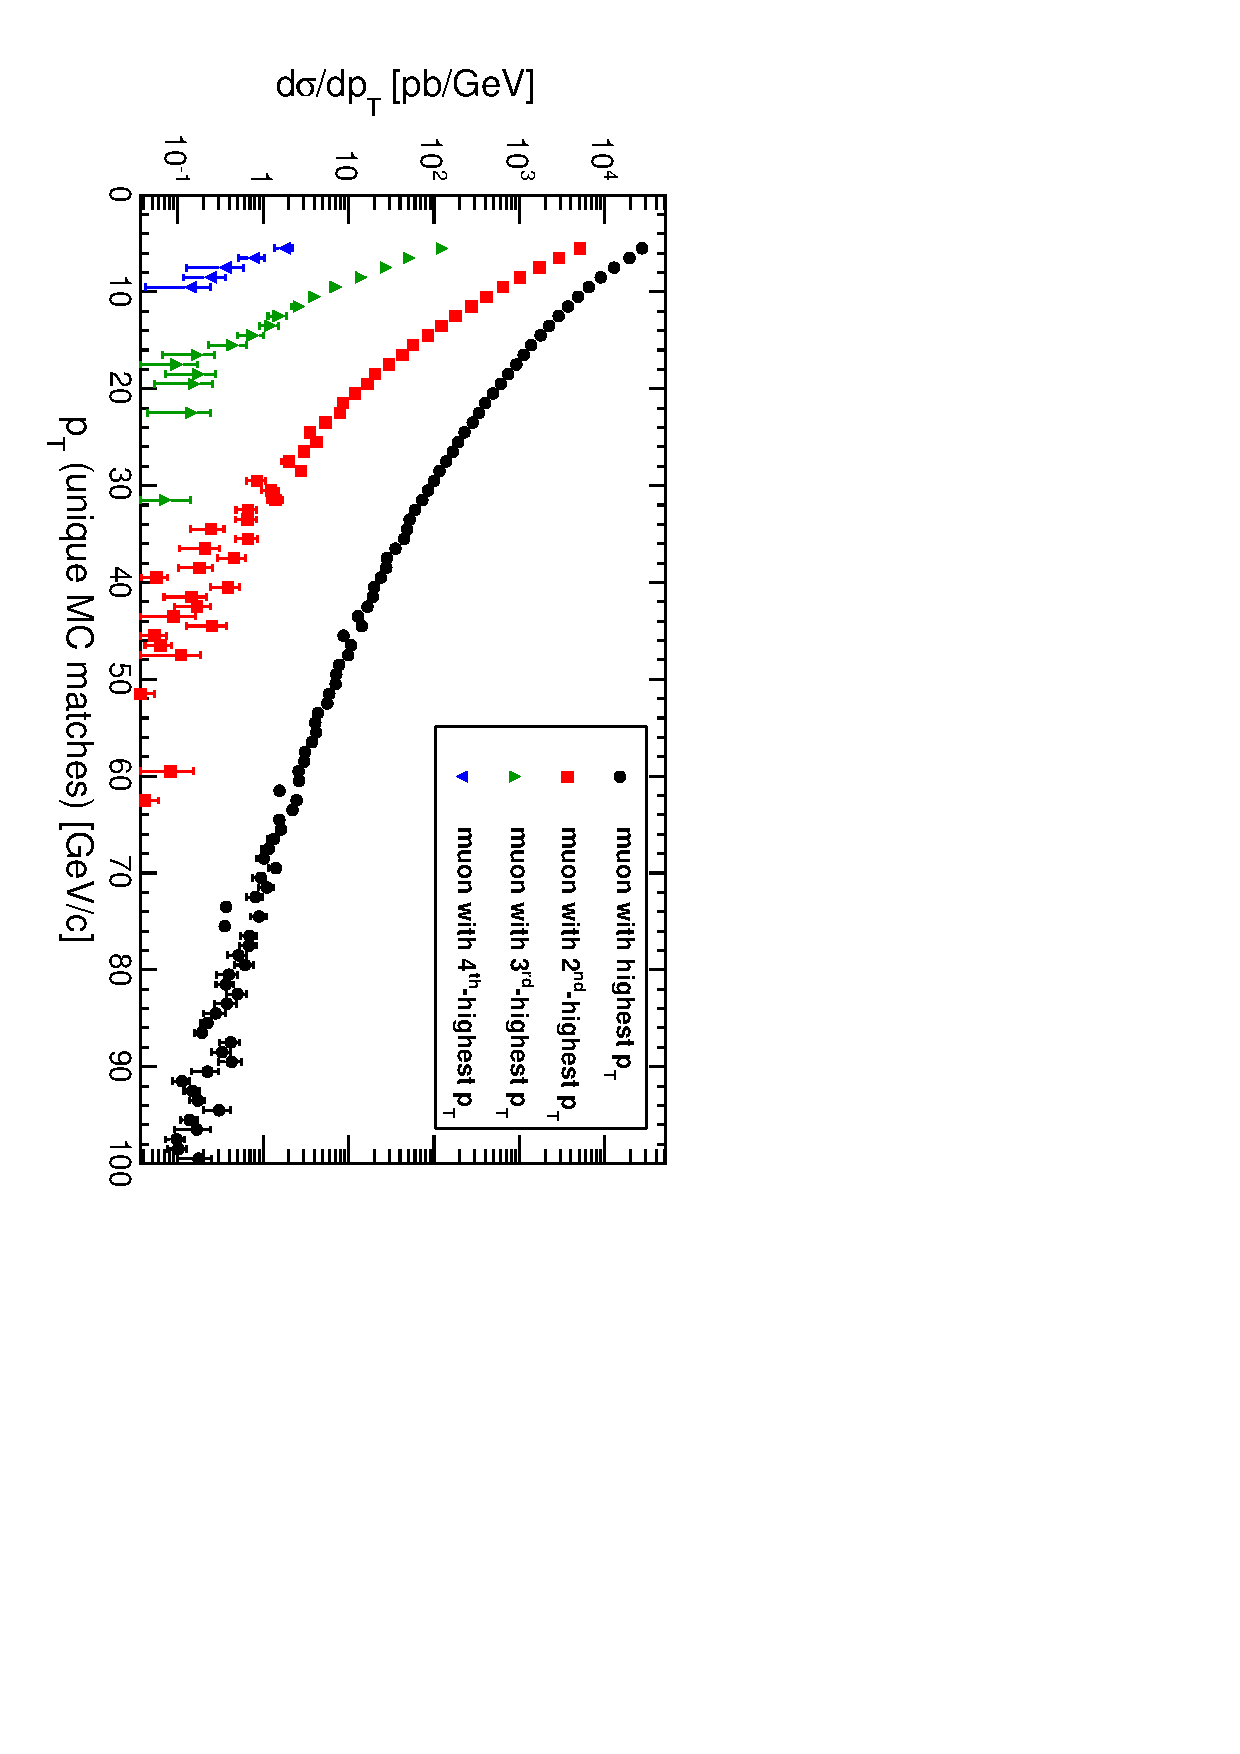
\includegraphics[height=0.5\linewidth, angle=90]{ptcurves_real.pdf}
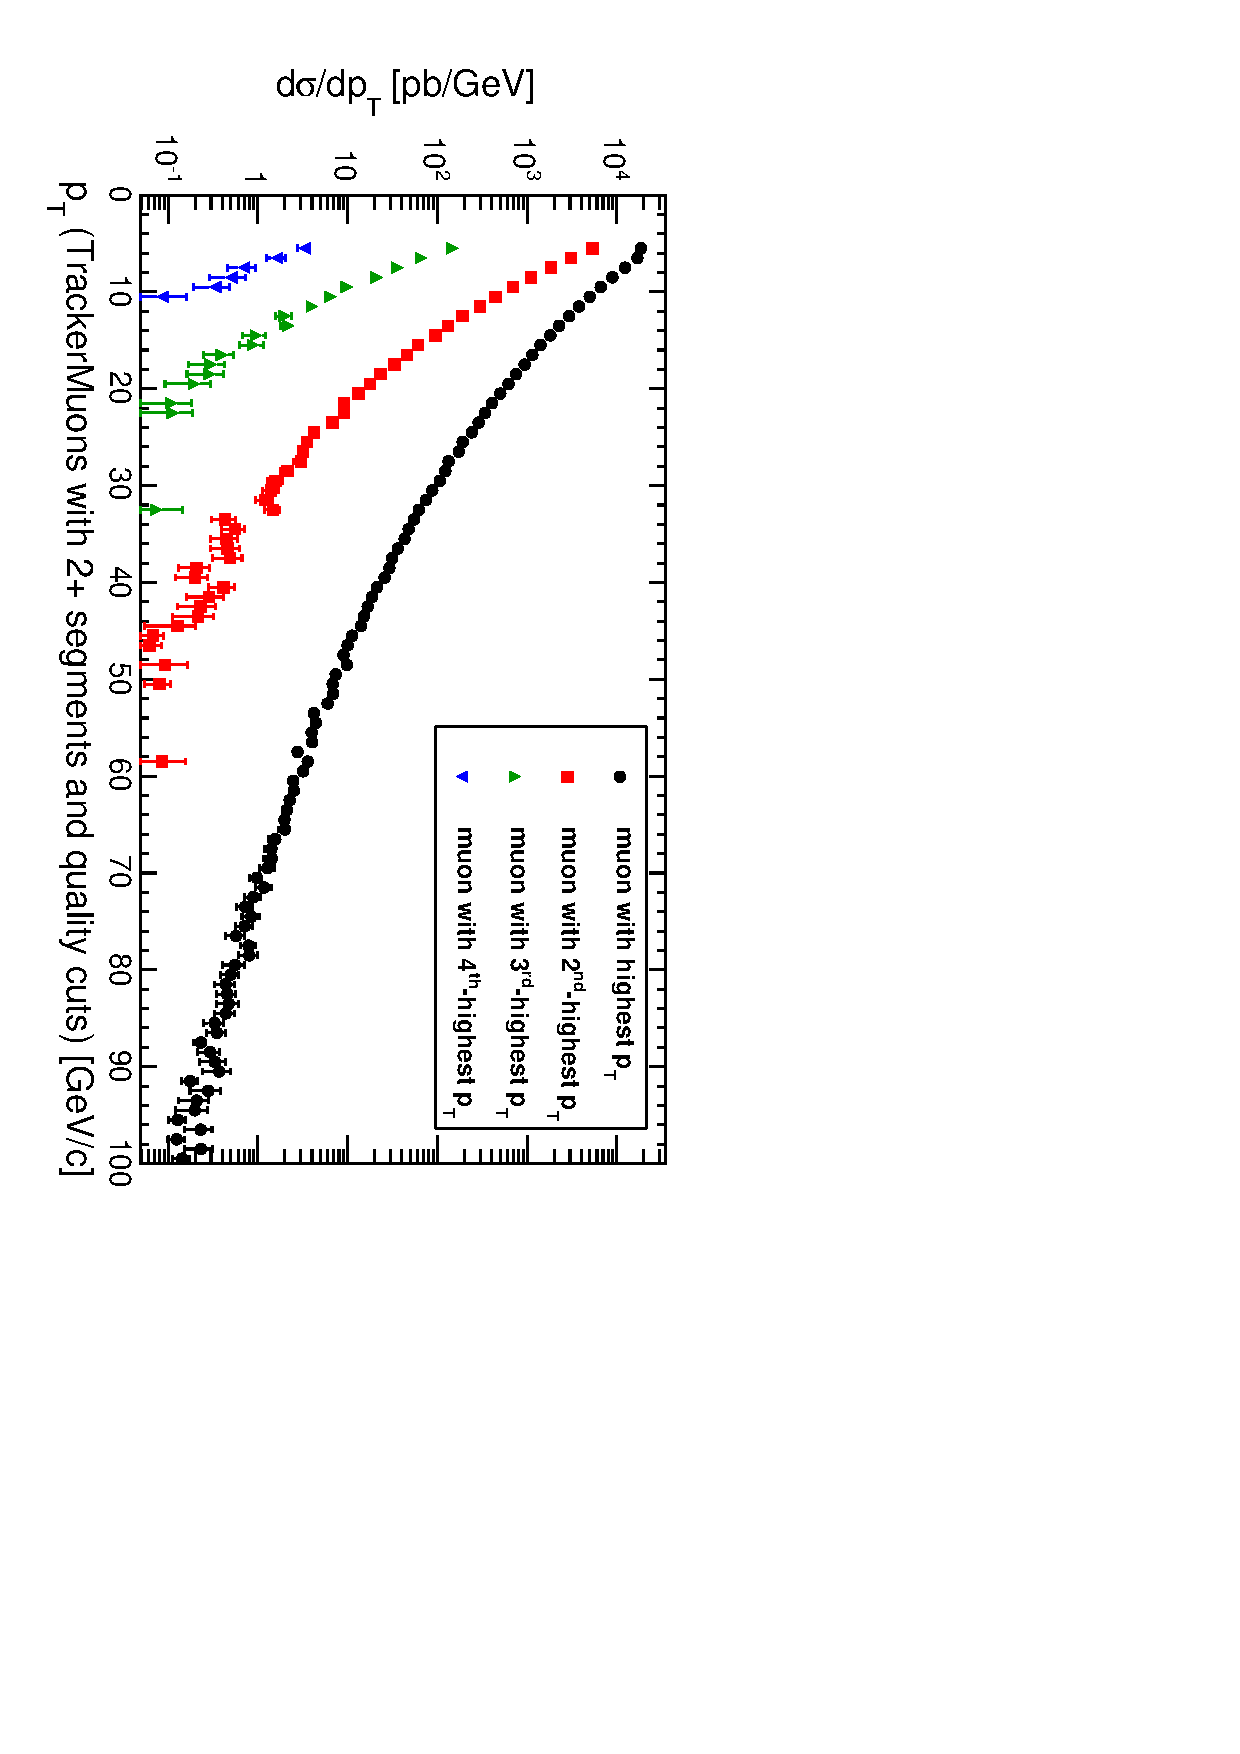
\includegraphics[height=0.3\linewidth, angle=90]{ptcurves_TwoChambersGoodTracker.pdf}
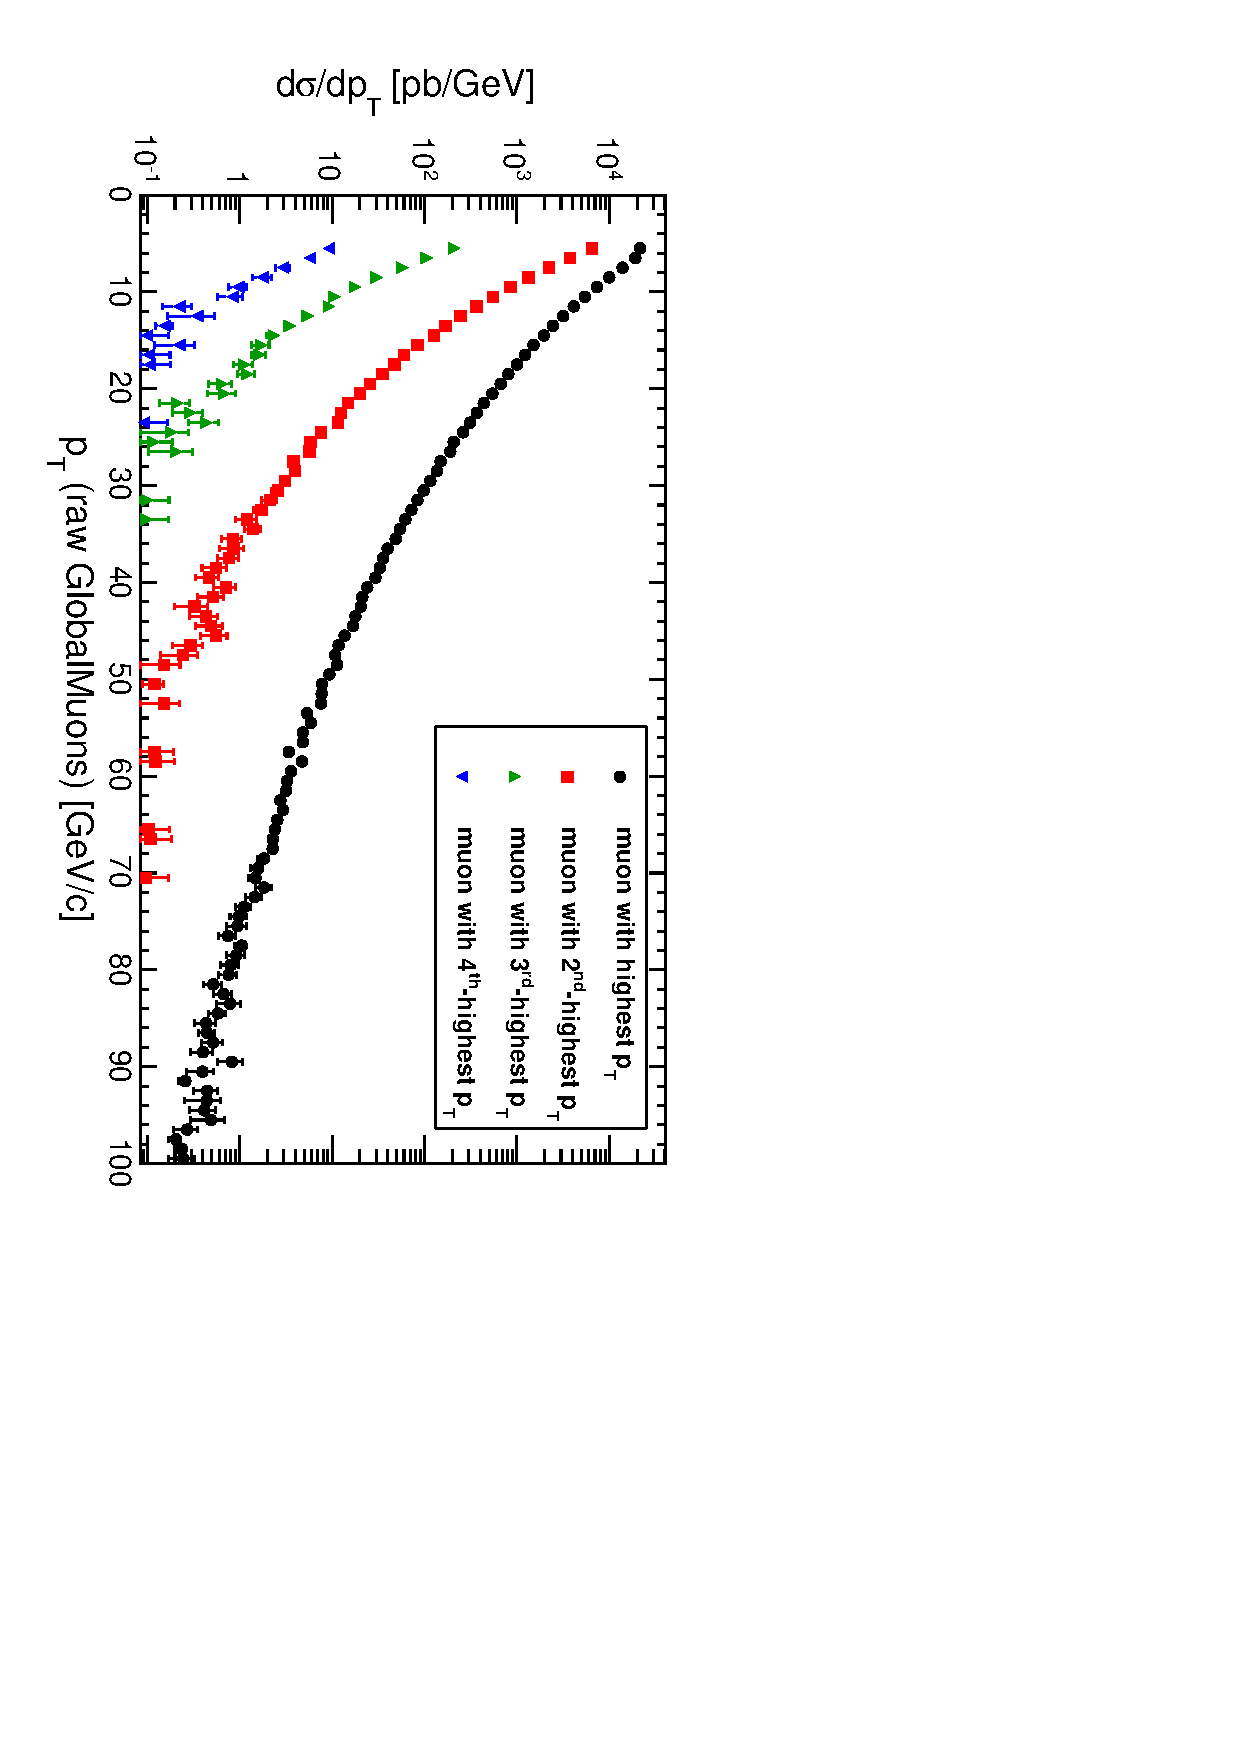
\includegraphics[height=0.3\linewidth, angle=90]{ptcurves_GlobalMuons.pdf}

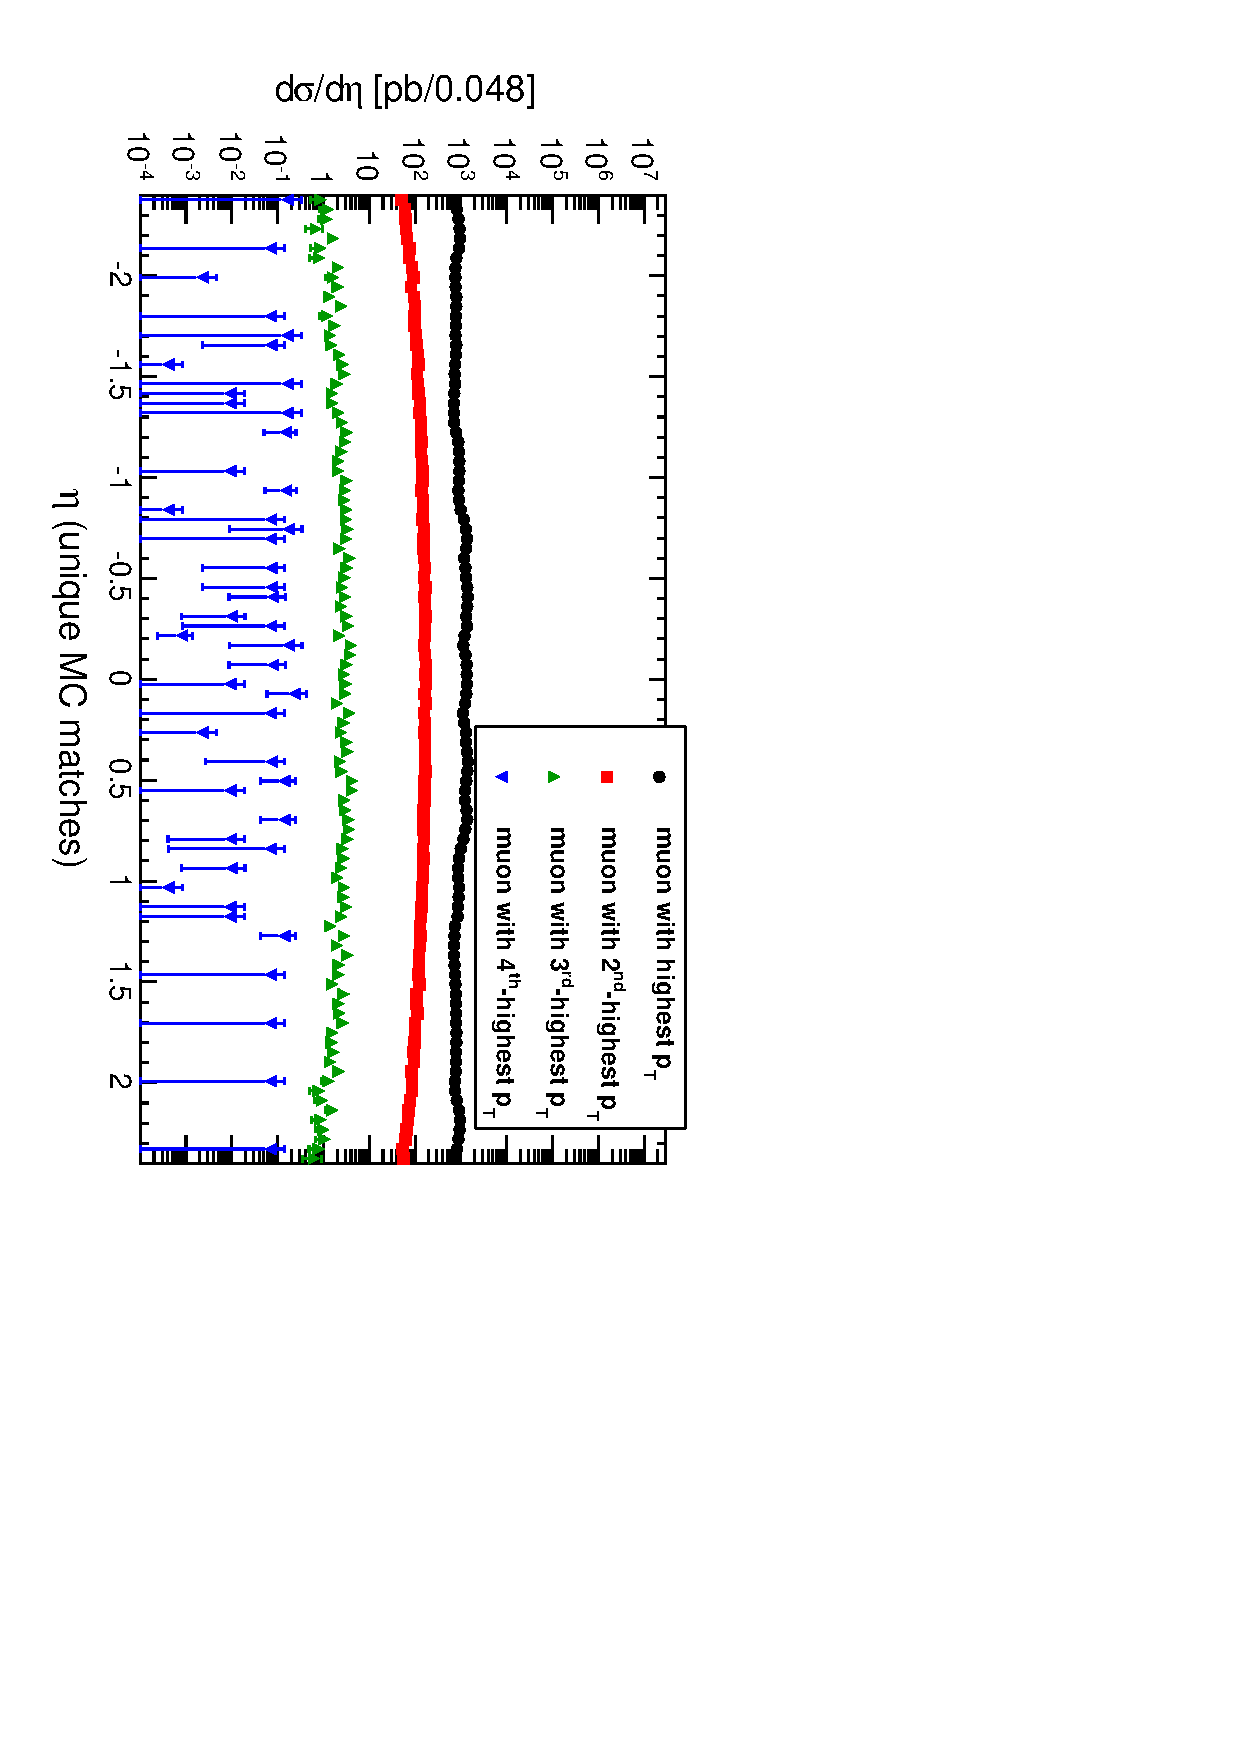
\includegraphics[height=0.5\linewidth, angle=90]{etacurves_real.pdf}
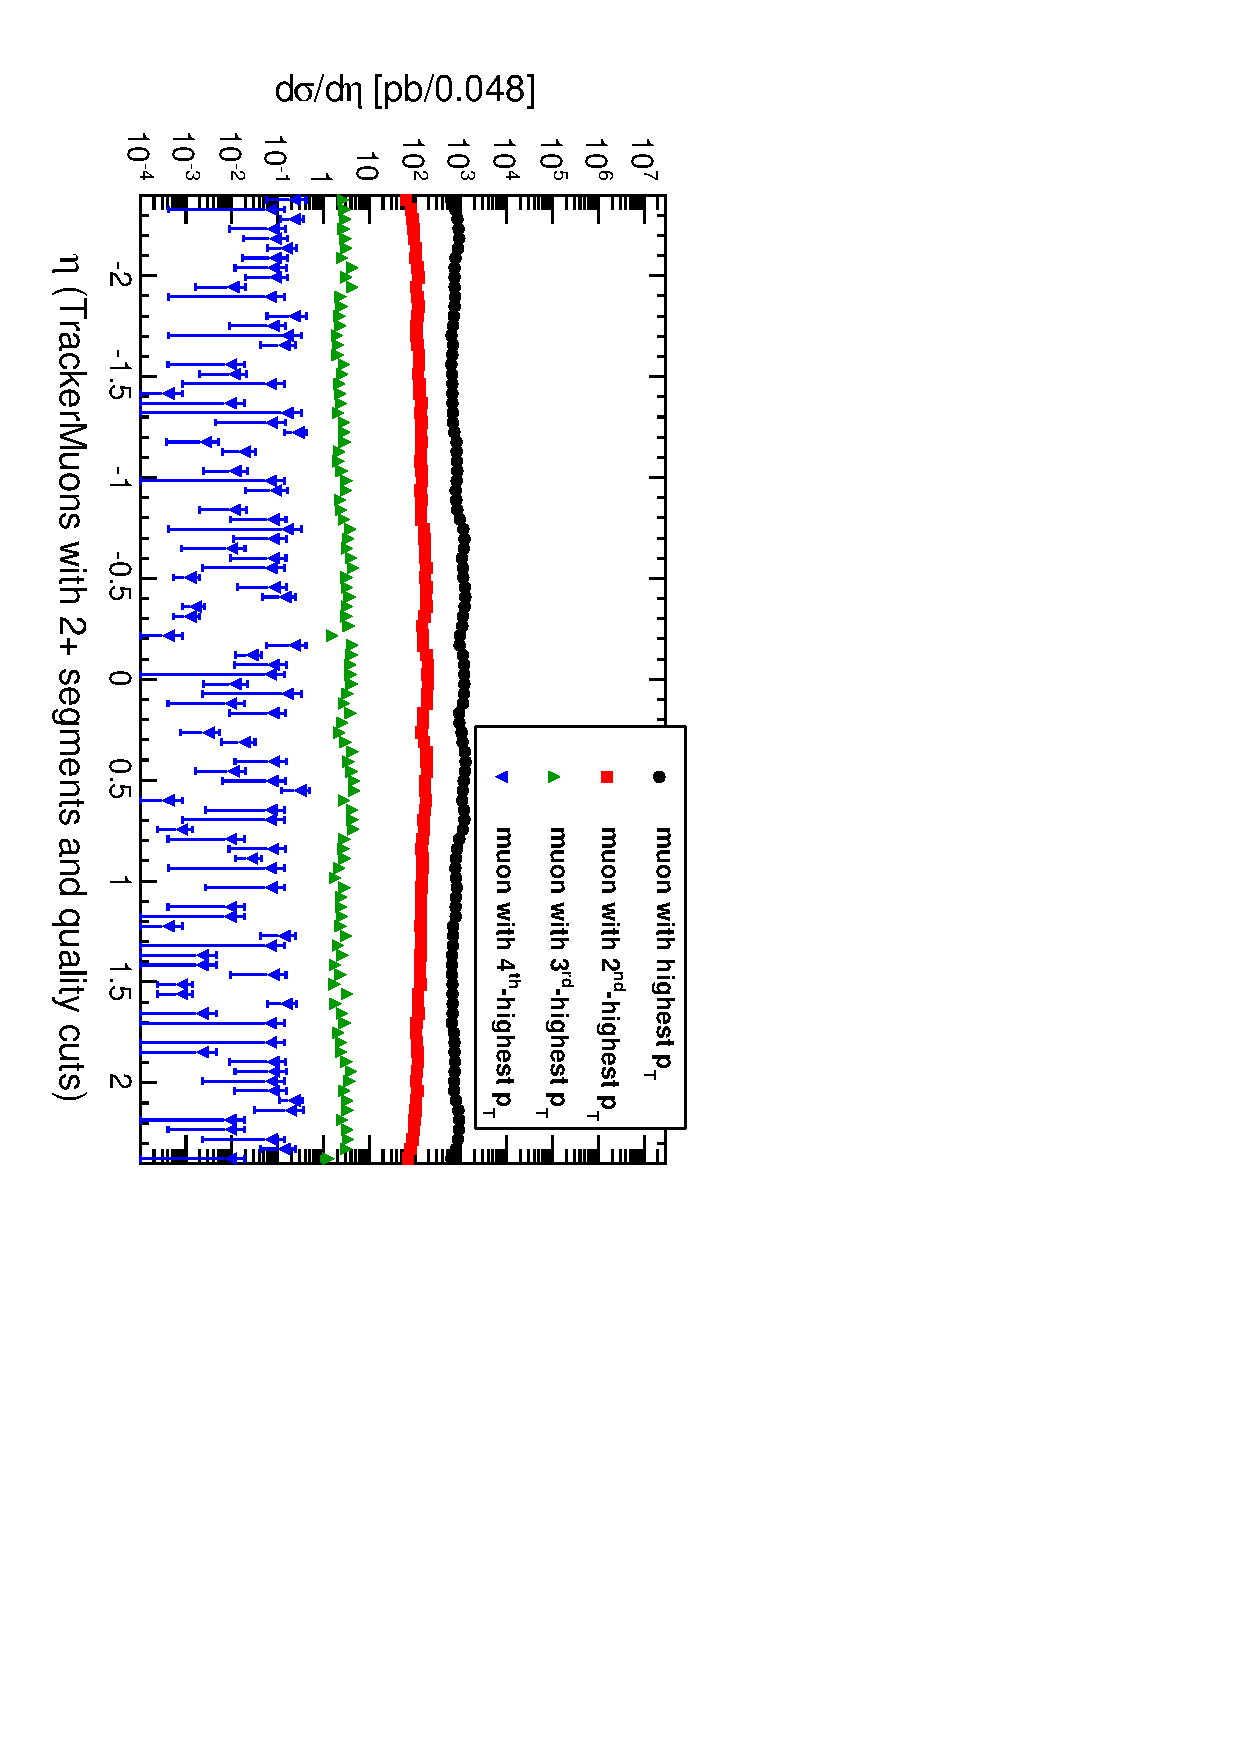
\includegraphics[height=0.3\linewidth, angle=90]{etacurves_TwoChambersGoodTracker.pdf}
\includegraphics[height=0.3\linewidth, angle=90]{etacurves_GlobalMuons.pdf}
\end{frame}

\begin{frame}
\frametitle{Backgrounds to muon-groups}

\begin{itemize}
\item Forming muon-groups with \textcolor{darkblue}{\only<1>{raw TrackerMuons}\only<2>{quality TrackerMuons}\only<3>{plain GlobalMuons}}
\item Where do the events come from? (6 disjoint gen-level categories)
\end{itemize}

\vfill
\only<1>{\includegraphics[height=0.5\linewidth, angle=90]{masslog_PlainTrackerMuonAny.pdf}
\includegraphics[height=0.5\linewidth, angle=90]{masslinear_PlainTrackerMuonAny.pdf}

\includegraphics[height=0.5\linewidth, angle=90]{ptlog_PlainTrackerMuonAny.pdf}
\includegraphics[height=0.5\linewidth, angle=90]{ptlinear_PlainTrackerMuonAny.pdf}}

\only<2>{\includegraphics[height=0.5\linewidth, angle=90]{masslog_QualityTrackerMuonAny.pdf}
\includegraphics[height=0.5\linewidth, angle=90]{masslinear_QualityTrackerMuonAny.pdf}

\includegraphics[height=0.5\linewidth, angle=90]{ptlog_QualityTrackerMuonAny.pdf}
\includegraphics[height=0.5\linewidth, angle=90]{ptlinear_QualityTrackerMuonAny.pdf}}

\only<3>{\includegraphics[height=0.5\linewidth, angle=90]{masslog_PlainGlobalMuonAny.pdf}
\includegraphics[height=0.5\linewidth, angle=90]{masslinear_PlainGlobalMuonAny.pdf}

\includegraphics[height=0.5\linewidth, angle=90]{ptlog_PlainGlobalMuonAny.pdf}
\includegraphics[height=0.5\linewidth, angle=90]{ptlinear_PlainGlobalMuonAny.pdf}}
\end{frame}

\begin{frame}
\frametitle{Number of $\mu$-groups}

\begin{columns}
\column{0.5\linewidth}
\includegraphics[height=\linewidth, angle=90]{groups_PlainTrackerMuonAny.pdf}

\includegraphics[height=\linewidth, angle=90]{groups_QualityTrackerMuonAny.pdf}

\includegraphics[height=\linewidth, angle=90]{groups_PlainGlobalMuonAny.pdf}

\column{0.5\linewidth}
\begin{itemize}
\item Background events with more than one $\mu$-group are at the level of 1--3~pb
\item Target for signals is at about the same level
\item So far, so good\ldots
\end{itemize}
\end{columns}
\end{frame}

\begin{frame}
\frametitle{Angle between $\mu$-groups}

\begin{itemize}
\item Expressed as an angle between two $\mu$-groups (0--$\pi$, left) or as a mass of all groups (right)
\item When you actually do have a second $\mu$-group in a background event, it seems to be uncorrelated with the first (they're not just wide sprays of muons being split into two nearby groups)
\end{itemize}

\includegraphics[height=0.5\linewidth, angle=90]{openingbypt_QualityTrackerMuonAny.pdf}
\includegraphics[height=0.5\linewidth, angle=90]{mall_QualityTrackerMuonAny.pdf}

\includegraphics[height=0.5\linewidth, angle=90]{openingbypt_PlainGlobalMuonAny.pdf}
\includegraphics[height=0.5\linewidth, angle=90]{mall_PlainGlobalMuonAny.pdf}
\end{frame}

\begin{frame}
\frametitle{$m_{12}$ vs.\ $m_{34}$ plots}
\framesubtitle{For cases in which both $\mu$-groups are coming from the same resonance}

Backgrounds:

\includegraphics[height=0.5\linewidth, angle=90]{m12m34bypt_QualityTrackerMuonAny.pdf}
\includegraphics[height=0.5\linewidth, angle=90]{m12m34bypt_PlainGlobalMuonAny.pdf}

\vfill
Signal (pair-pair gun with uniformly distributed mass):

\includegraphics[height=0.5\linewidth, angle=90]{m12m34.pdf}
\includegraphics[height=0.5\linewidth, angle=90]{mdiff_vs_mass.pdf}
\end{frame}

\begin{frame}
\frametitle{Isolation}

\begin{itemize}
\item Background (left) compared with NMSSM signal (right)
\item Similar distributions for dimuon-gun with pile-up and Extra-$\mathcal{U}(1)$ model, but my script over-wrote them!
\item NMSSM vertical axis is wrong (it's number of events in the sample, not anything to do with ``pb'')
\end{itemize}

\includegraphics[height=0.5\linewidth, angle=90]{tkisolation_QualityTrackerMuonAny.pdf}
\includegraphics[height=0.5\linewidth, angle=90]{tkisolation_QualityTrackerMuonAny_NMSSM.pdf}

\includegraphics[height=0.5\linewidth, angle=90]{tkisolation_PlainGlobalMuonAny.pdf}
\includegraphics[height=0.5\linewidth, angle=90]{tkisolation_PlainGlobalMuonAny_NMSSM.pdf}
\end{frame}

\begin{frame}
\frametitle{Relative isolation}

\begin{itemize}
\item Even better separation of signal and background (need to zoom in)
\end{itemize}

\includegraphics[height=0.5\linewidth, angle=90]{tkrelisolation_QualityTrackerMuonAny.pdf}
\includegraphics[height=0.5\linewidth, angle=90]{tkrelisolation_QualityTrackerMuonAny_NMSSM.pdf}

\includegraphics[height=0.5\linewidth, angle=90]{tkrelisolation_PlainGlobalMuonAny.pdf}
\includegraphics[height=0.5\linewidth, angle=90]{tkrelisolation_PlainGlobalMuonAny_NMSSM.pdf}
\end{frame}

\begin{frame}
\frametitle{Displaced vertices}

\begin{itemize}
\item Backgrounds fall off very quickly as a function of displaced vertex (except raw TrackerMuons, which are contaminated by muons from decays-in-flight)
\item Unfortunately, the final plot got drawn in linear scale (need to fix)
\item More unfortunately, the choice of quality cuts has low efficiency for highly displaced vertices (I need to check and possibly fix it)
\end{itemize}

\includegraphics[height=0.45\linewidth, angle=90]{dispvert_QualityTrackerMuonAny.pdf}
\includegraphics[height=0.45\linewidth, angle=90]{dispvert_eff_QualityTrackerMuonAny.pdf}

\includegraphics[height=0.45\linewidth, angle=90]{dispvert_PlainGlobalMuonAny.pdf}
\includegraphics[height=0.45\linewidth, angle=90]{dispvert_eff_PlainGlobalMuonAny.pdf}
\end{frame}

%% \begin{frame}
%% \frametitle{Outline}
%% \begin{itemize}\setlength{\itemsep}{0.75 cm}
%% \item 
%% \end{itemize}
%% %% \hspace{-0.83 cm} \textcolor{darkblue}{\Large Outline2}
%% \end{frame}

%% \section*{First section}
%% \begin{frame}
%% \begin{center}
%% \Huge \textcolor{blue}{First section}
%% \end{center}
%% \end{frame}

\begin{frame}
\frametitle{Conclusions}

Work in progress!

\label{numpages}
\end{frame}

\end{document}
